\documentclass[11pt,a4paper]{amsart}
\usepackage[margin=1in]{geometry}
\usepackage{amsmath,amssymb,amsthm,mathtools,mathrsfs}
\usepackage[expansion=false]{microtype}
\usepackage{tikz}
\usepackage[colorlinks=true,linkcolor=black,citecolor=black,urlcolor=black]{hyperref}
\usepackage[nameinlink,capitalize]{cleveref}
\hypersetup{
 pdftitle={Recognition of ribbon-outer skew Schur compositions},
 pdfauthor={John Shields},
 pdfkeywords={skew Schur function, marked composition, source-minimal factorization, ribbon outer, prescribed fiber, Jacobi--Trudi determinant, boundary reconstruction}}
\pdfinfo{/ORCID (https://orcid.org/0009-0004-3882-4571)}
\numberwithin{equation}{section}
\theoremstyle{plain}
\newtheorem{theorem}{Theorem}[section]
\newtheorem{proposition}[theorem]{Proposition}
\newtheorem{lemma}[theorem]{Lemma}
\newtheorem{corollary}[theorem]{Corollary}
\theoremstyle{definition}
\newtheorem{definition}[theorem]{Definition}
\newtheorem{remark}[theorem]{Remark}
\newtheorem{example}[theorem]{Example}
\newcommand{\Lam}{\Lambda}
\newcommand{\Z}{\mathbb Z}
\newcommand{\Q}{\mathbb Q}
\newcommand{\one}{\mathbf1}
\newcommand{\AT}{\operatorname{AT}}
\newcommand{\Row}{\operatorname{Row}}
\newcommand{\Col}{\operatorname{Col}}
\newcommand{\spn}{\operatorname{sp}}
\newcommand{\ord}{\operatorname{ord}}
\newcommand{\JT}{\operatorname{JT}}
\newcommand{\Jlower}{\mathsf J_{<n}}
\newcommand{\Vop}{\mathcal V}
\newcommand{\ii}{\iota}

\title[Ribbon-outer recognition]{Recognition of ribbon-outer\\skew Schur compositions}
\author{John Shields}
\date{October 22, 2026}
\thanks{Independent researcher, Ginza 2-15-2, KR Ginza II 5F, Chuo-ku, Tokyo, Japan 104-0061.\\
\hspace*{\parindent}Corresponding author: \href{mailto:math@johnnyshields.com}{math@johnnyshields.com}.  ORCID: \href{https://orcid.org/0009-0004-3882-4571}{0009-0004-3882-4571}.\\
\hspace*{\parindent}This work is archived at \href{https://doi.org/10.5281/zenodo.23644527}{doi:10.5281/zenodo.23644527}.}
\subjclass[2020]{Primary 05E05; Secondary 05A17, 15A15}
\keywords{skew Schur function, marked composition, source-minimal factorization,
ribbon outer, prescribed fiber, Jacobi--Trudi determinant, boundary reconstruction}

\begin{document}
\begin{abstract}
We prove a recognition theorem for skew diagram compositions satisfying
Hypotheses I--IV of McNamara and van Willigenburg.  The inner diagram
carries two translated end copies of an overlap, or boundary edges for
an empty overlap, and their attachments; the period is their content
displacement.  A composition is proper when both factors are connected
and have at least two cells.  Minimality at a fixed parent first
minimizes the overlap's diagonal span, then the inner diagram's.
For Schur-equal minimal compositions of diagrams with at least 24 cells,
assume the first has a ribbon outer and no smaller period.
We recover its marked inner and outer Schur function on the other diagram,
up to rotation of the full marking data and permitted attachment changes
with their outer involution.  The original Schur class contains no proper
row- or column-inner composition.  At every smaller cell count, we assume
that proper-composition existence transfers under Schur equality, every
class with more than one rotation orbit contains a proper composition,
and Schur-equal minimal compositions have the same marked inner and
outer Schur function modulo these identifications.  A finite Jacobi--Trudi
identity and two boundary records construct the legal factors before
minimality is applied.
\end{abstract}
\maketitle

\section{Introduction}\label{sec:introduction}

The skew diagram composition of McNamara and van Willigenburg
\cite{McNamara2009Classification} assembles translated copies of a connected
inner diagram \(E\) according to a connected outer diagram \(D\).
The end data specify two copies of an overlap \(W\), their displacement,
and their horizontal or vertical attachments.  For nonempty \(W\), the
copies contain the southwest and northeast cells of \(E\); for empty
\(W\), the marks are boundary edges.  We retain \(E\) and these data as a
\emph{marked inner} \(\omega\) and write \(D\circ_\omega E\), following
\cite{Shields2026Gluing}.  Different assemblies can have the
same skew Schur function \cite{Reiner2007Coincidences}.  The recognition
problem asks whether that function determines a prescribed marked inner,
rather than only its Schur function.
A \emph{Schur class} consists of connected diagrams with the same
skew Schur function.

Under Hypotheses I--IV of McNamara and van Willigenburg, composition
and factor reversal preserve skew Schur equality, by Olson-Harris's
theorems \cite{OlsonHarris2024HopfApplications}.  The earlier results of
McNamara and van Willigenburg imposed the additional attachment restriction
of Hypothesis V \cite{McNamara2009Classification}.
A marking is \emph{legal} if it satisfies I--IV.

Following \cite{Shields2026Gluing}, a \emph{chart} of \(F\) is a chosen
legal composition presentation \(F=D\circ_\omega E\), including its full
marking data.  It is \emph{proper} when both connected factors have at
least two cells.  The converse problem requires such charts on the
diagrams being compared.  A factor of a determinant does not supply a chart.
A \emph{line-inner} chart has an inner that is a single row or column.
In a \emph{ribbon-outer} chart, \(D\) is a ribbon; the whole diagram
\(F\) need not be one.

The content of a cell \((i,j)\) is \(j-i\).  If translation by
\(v=(v_1,v_2)\) sends the lower end mark to the upper one, the
\emph{period} is their content displacement \(p=v_2-v_1\)
\cite{Shields2026Gluing}.  Write \(N_A\) for the number of occupied
content diagonals of a diagram \(A\), and \(w=N_W\) for the
\emph{overlap width}, with \(w=0\) for the empty overlap.  Then
\begin{equation}\label{eq:intro-span}
 N_E=p+w,\qquad N_F=pN_D+w,\qquad 0\le w<p.
\end{equation}
A chart is \emph{source-minimal} when its score \((w,N_E)\) is lexicographically
least among all proper charts of that same parent.  This is the
minimal-factorization convention of McNamara and van Willigenburg
\cite{McNamara2009Classification}.  The qualifier \emph{source} specifies
that the parent \(F\) is held fixed, rather than varied over its Schur
class \cite{Shields2026Gluing}.

The attachments are \emph{ordinary} when both are horizontal or both
vertical, and \emph{mixed} when they differ.  A permitted \emph{gauge
change} switches between two legal ordinary markings of the same inner,
or between the corresponding empty-edge readings, together with the
fundamental involution on the outer Schur function.

The \emph{prescribed full marked fiber} \(\mathcal F(\omega,s_D)\) is
the set of diagrams admitting proper compositions through the fixed
marked inner \(\omega\), or its transported rotation, with outer Schur
function \(s_D\) \cite{Shields2026Gluing}.  Transported rotation means
a half-turn of the inner and both end marks, interchanging the lower
and upper ends and transporting their attachments.  The fiber includes
the permitted gauge changes with their action on the outer function;
the markings are not identified while that function is held fixed.
Precise conventions are given in \Cref{sec:charts}.

A diagram is \emph{rooted} if it has a proper chart.  The \emph{key}
of a source-minimal chart is its full marked inner and outer Schur
function, modulo the rotations and gauges just described
\cite{Shields2026Gluing}.  Area means the number of occupied cells.
For the original cell count \(n\), we use the joint smaller-area
hypothesis \(\Jlower\) of \cite{Shields2026RibbonPeriod}.
At each Schur class of area strictly less than \(n\), we assume that
one rooted member implies all members are rooted; that a class with
more than one rotation orbit contains a rooted member; and that
rooted members have the same source-minimal key.
No assertion at area \(n\) is included.

\begin{theorem}[Ribbon-outer recognition]\label{thm:recognition}
Let \(n\ge24\), and assume \(\Jlower\).  Let
\begin{equation}\label{eq:original-charts}
 F=D\circ_\omega E,\qquad H=C\circ_\eta U,\qquad
 s_F=s_H,\qquad |F|=n
\end{equation}
be actual proper source-minimal charts satisfying Hypotheses I--IV of
McNamara and van Willigenburg.
Let their periods be \(p\ge q\), respectively.  Suppose \(D\) is a
ribbon and no member of their whole Schur class has a proper line-inner
chart.  Then \(p=q\) and
\begin{equation}\label{eq:main-fiber}
 H\in\mathcal F(\omega,s_D).
\end{equation}
The fiber is prescribed by the original displayed chart of \(F\).
Its only identifications are transported full-mark rotation and the
genuine ordinary or empty-overlap gauge, with its action on the outer
function.
\end{theorem}

The period equality is the ribbon-outer period-rigidity theorem of
\cite{Shields2026RibbonPeriod}, under exactly these original chart and
strictly smaller-area hypotheses.  Once the periods agree, the assertion
proved here constructs a proper chart of \(H\) through the prescribed
marked inner of \(F\), with outer function \(s_D\), up to the full-mark
rotations and gauges above.  Equal widths follow from
\eqref{eq:intro-span}; an extreme Jacobi--Trudi cofactor comparison makes
\(C\) a ribbon as well \cite{Shields2026CornerDescent}.
The result does not assert uniqueness of all factorizations,
choose a new fiber after the comparison, or supply rootedness transfer or
root existence at the current area.

Two distinctions govern the proof.  First, factor-function recovery is not
marked-factor recovery.  The ordinary and mixed ribbon inverses at a
supplied period are the factor-recovery theorems of
\cite{Shields2026Readout}.  They use Hall adjoints and a weighted derivation, respectively.
If the recovered inner function has several realizations, its full mark
has still to be placed on the second diagram.  Where the proof also
supplies the function of a first-row deletion, reconstruction from these
two boundary observations identifies the connected diagram up to
translation \cite[Reconstruction from two boundary observations]{Shields2026SkewSchur}.
Second, same-parent gluing
compares charts that already exist on one diagram
\cite{Shields2026Gluing}.  It cannot supply the missing chart on another
Schur-equal parent.

Corner descent compares the extreme Jacobi--Trudi cofactors.  The interior
of a diagram consists of the northwest cells of its \(2\times2\) blocks.
The corner transport theorem \cite{Shields2026CornerDescent} records the
compositions arising from connected components of the outer interior
inside the whole composition's cofactor.  A ribbon has no \(2\times2\)
block, so this descent provides no outer-interior child composition.

Instead, we compare compositions whose outer diagram is a horizontal or
vertical domino.  For a nonline inner, outer-independent minimality
\cite{Shields2026CornerDescent} preserves a source-minimal chart when its
connected proper outer is changed.  Whenever these test diagrams have fewer cells,
\(\Jlower\) settles the comparison; the remaining original outers have
two cells.  If the recovered inners \(E\) and \(U\) are not related by
rotation, they themselves have fewer than \(n\) cells.
The hypothesis \(\Jlower\) then gives compositions of \(E\) and \(U\)
through the same full marked inner.  These are the \emph{finer charts}:
they factor the inner diagrams themselves.
The remaining algebra compares the Jacobi--Trudi determinants of the finer
outer diagrams, retaining the complete inverse matrices in each chart's
own rational coordinates.

On the mixed branch, the composition equality supplies a finite identity
for rational coefficient functions describing permitted variations of
these determinants.  At the actual private gate, the aliases and fine
weight make a nonzero response a positive integer power of the returned
clock with constant rational amplitude.  Whole-field stationary descent
\cite[Whole moving potential]{Shields2026Coframes} excludes such a response
on distinct equal-function diagrams.  Its use here requires the actual
coarse span, raw independence in each rebuilt field, the full moving
homomorphism, and every coefficient through the terminal degree.
These are supplied by the physical comparison, not assumed as an
algebraic replacement for it.  The resulting vanishing coefficient is
not yet a geometric factorization.

Substituting this vanishing coefficient into the two-copy identity
produces connected diagrams with equal whole Schur functions and strictly
fewer cells.  Only after these smaller diagrams have been constructed is
\(\Jlower\) applied to them.  Their two boundary words, the binary step
records of the northwest and southeast boundaries, supply the native
hypotheses of the decoder and residue folds in \cite{Shields2026Gluing}.
Those constructions retain I--IV, both full end marks and their
attachments.  The resulting period divides that of the finer charts.
The aligned composition theorem \cite{Shields2026Gluing} then places a new chart on
the same diagram at which the relevant source minimum was chosen.
Only this realized chart's score is compared with the minimum.
The ordinary and mixed attachment cases require different boundary
arguments.

\Cref{sec:charts} fixes the chart and descent conventions.
\Cref{sec:reduction} gives factor readout, the literal-inner finish,
the reduction to two-cell outers, and then the nonliteral common finer source.
\Cref{sec:comparison} derives the actual finite equations and applies
coframe separation \cite{Shields2026Coframes}.
\Cref{sec:children} specifies the imported geometric interfaces;
\Cref{sec:boundary} constructs their actual inputs and outputs,
and \Cref{sec:completion} completes recognition.
The appendices prove the physical determinant identities, exceptional
cell constructions, and complete finite comparisons used by these reductions.

\section{Marked charts and strict descent}\label{sec:charts}

\subsection{Diagrams and the two boundary words}

Diagrams are finite skew Young diagrams in English notation, identified up to translation.  Connected means nonempty and edge-connected.  The area \(|S|\) is the number of cells; \(N_S\) is the number of occupied content diagonals.  The content of \((i,j)\) is \(j-i\), and \(e=(1,1)\).  For connected diagrams, \(N_S=r(S)+c(S)-1\).  We write \(S^*\) for rotation through \(180\) degrees and \(\AT(i,j)=(-j,-i)\).  The involution \(\ii\) on symmetric functions satisfies \(\ii(h_j)=e_j\) and \(\ii(s_S)=s_{\AT(S)}\).  A line is a row or column; a ribbon is a connected diagram without a \(2\times2\) block.

We work in \(\Lam=\Q[h_1,h_2,\ldots]\), with \(h_0=1\) and \(h_j=0\) for \(j<0\).  A southwest-normalized connected diagram of span \(N\) has full beta lists
\begin{equation}\label{eq:full-flags}
 X=(N,x_1,\ldots,x_{r-1}),\qquad
 Y=(y_0,\ldots,y_{r-2},0),\qquad
 s_S=\det(h_{x-y})_{x\in X,\,y\in Y},
\end{equation}
with both lists strictly decreasing.  Equal labels in the two lists are retained.  They correspond to actual unit entries, not to deleted cells.

If \([\ell_k,h_k]\) is the row interval on content \(k\), define
\begin{equation}\label{eq:boundary-words}
 A_k=\ell_{k-1}-\ell_k=\one_{k\in Y},\qquad
 B_k=h_{k-1}-h_k=\one_{k\in X},\qquad 1\le k<N.
\end{equation}
Both words are binary.  Their height is
\begin{equation}\label{eq:height}
 H_S(k)=h_k-\ell_k+1
 =\#\{y\in Y:y\le k\}-\#\{x\in X:x\le k\},
 \qquad H_S(k)-H_S(k-1)=A_k-B_k.
\end{equation}
There are no artificial steps at \(0\) or \(N\).  The height word alone forgets the distinction between the pairs \((0,0)\) and \((1,1)\).

\begin{lemma}\label{lem:diagonal-reconstruction}
A finite cell set is a connected skew diagram if its contents form an interval, each diagonal is a row interval, its two endpoint sequences have steps zero or minus one, and its extreme diagonals are singletons.  Conversely, every connected skew diagram has these properties.  Thus positive heights with singleton ends and the two binary boundary words determine a connected skew diagram up to translation.
\end{lemma}
\begin{proof}
Starting from the southwest singleton, the two words successively give the endpoints of every diagonal interval.  The step conditions are exactly the two skew-boundary conditions.  Every cell outside the last diagonal has an eastern or northern neighbor on the next diagonal: the next interval contains either its row or the preceding row.  Hence the set is edge-connected.  The converse follows by following the two boundaries of a connected skew diagram.
\end{proof}

The area, row count, column count, span, and row-overlap multisets are Schur invariants \cite{Reiner2007Coincidences}.  Connected skew Schur functions are irreducible \cite{Barekat2009CoincidencesCorrigendum}.  We use primitivity in the complete generators to fix scalar normalizations.  The interior
\(S^- =\{x\in S:x+e\in S\}\) satisfies
\begin{equation}\label{eq:corner}
 (-1)^{r(S)-1}[h_{N_S}]s_S=s_{S^-}.
\end{equation}
The right side is the product of the Schur functions of its connected components.  This is the extreme cofactor in \eqref{eq:full-flags}.

\subsection{Full legal marks}

A marked inner \(\omega\) consists of a connected diagram \(E\), two congruent connected end diagrams \(W_-\) and \(W_+=W_-+v\), and their attachment case.  The lower copy contains the southwest cell of \(E\), the upper copy its northeast cell.  Put
\[
 O=E\setminus(W_-\cup W_+),\qquad w=N_W,\qquad p=c(v)=N_E-w.
\]
The four cases, listed as lower and upper attachments, are
\begin{equation}\label{eq:cases}
 \begin{array}{c|cccc}
 \text{case}&\mathrm{(a)}&\mathrm{(b)}&\mathrm{(c)}&\mathrm{(d)}\\\hline
 \text{attachments}&(H,H)&(V,V)&(H,V)&(V,H).
 \end{array}
\end{equation}
Cases (a) and (b) are ordinary; cases (c) and (d) are mixed.  A horizontal lower attachment uses the western neighbor of the southwest cell of \(O\), and a vertical lower attachment its southern neighbor.  The upper attachments use the eastern or northern neighbor of the northeast cell of \(O\).

We use the following complete form of Hypotheses I--IV \cite{McNamara2009Classification,Shields2026Gluing}.
\begin{enumerate}
\item[(I)] No strictly larger skew diagram containing \(W_-\) on the same content diagonals has translates at both ends of \(E\).
\item[(II)] There is an occupied diagonal between the two copies meeting neither: \(0\le w<p\).
\item[(III)] Removing either end copy leaves a connected skew diagram.
\item[(IV)] In \(\boldsymbol E=\bigcup_{k\in\Z}(E+kv)\), no hatted-middle copy is adjacent to a hatted-mark copy, where
\begin{equation}\label{eq:full-hats}
 \widehat O_1=\{x\in O_1:x+e\in O_1\},\qquad
 \widehat W_1=\{x\in\boldsymbol E:x+e\in W_1\}
 \cup\{x\in W_1:x+e\in\boldsymbol E\}.
\end{equation}
Both sets in the union and every integer translate are included.  Adjacency means sharing an edge.
\end{enumerate}
At width zero the mark is read horizontally: the west edge of the southwest cell and the east edge of the northeast cell have displacement
\(v_H=\operatorname{ne}(E)-\operatorname{sw}(E)+(0,1)\).
The vertical reading has \(v_V=v_H-e\) and is converted by the genuine gauge below.  Hypothesis V is not imposed.

For completeness, the cells in a composition can be described directly.  If the outer diagonal \(j\) has row interval \([\ell_j,h_j]\), the copy indexed by \(d=(i,i+j)\) has origin
\begin{equation}\label{eq:copy-origins}
 L_\omega(d)=
 \begin{cases}
 jv+ie,&\mathrm{(a)},\\
 jv-ie,&\mathrm{(b)},\\
 jv+(i-\ell_j)e,&\mathrm{(c)},\\
 jv-(h_j-i)e,&\mathrm{(d)}.
 \end{cases}
\end{equation}
In case (c), respectively (d), a vertical pair on the same northwest, respectively southeast, boundary ribbon contributes the supplemental copy
\(W_++L_\omega(d)+e\), respectively \(W_++L_\omega(d)-e\), with \(d\) the lower cell.  These copies are part of the definition.  A proper chart has connected \(D,E\) with \(|D|,|E|\ge2\).

\begin{proposition}\label{prop:local-data}
For a positive-width legal mark, \(W_-=E\cap(E-v)\).  The middle is thin on the marked diagonals, and the private diagonals \(w\) and \(p-1\) are singletons.  Its middle content interval has the form \([s,p+t-1]\), with \(1\le s\le w\), \(0\le t<w\); in the mixed cases \(t<s\).  A composition of outer span \(m\) has span \(mp+w\).  Its first and last \(p\) diagonals determine the inner, with the final copy translated by \((m-1)v\) in the mixed cases.
\end{proposition}
\begin{proof}
These are the local geometry and copy-placement statements of \cite[Lemma \textup{(local geometry)}]{Shields2026Gluing}.  Here are the points used in subsequent constructions.  The intersection \(E\cap(E-v)\) is skew and contains the supplied connected end copy on every marked diagonal; maximality gives equality.  If a middle tail first has two cells on a marked diagonal, its northwest cell is hatted-middle and is edge-adjacent to the hatted mark on the preceding diagonal.  This contradicts IV.  At the first private diagonal either III gives a new extreme singleton, or the same adjacency excludes a second cell; rotation gives the other private singleton.  In a mixed mark the two thin tails cannot overlap at a relative marked content, by the full-intersection assertion, and the endpoint attachment rules exclude equality of their total span with \(p\).  Thus \(t<s\).  Finally, \eqref{eq:copy-origins} gives the span and the two extreme windows.  The private singleton in their overlap fixes the joining translation.
\end{proof}

We use the coding theorem of \cite[Boundary coding lemma]{Shields2026Gluing} with its endpoint convention.  The only possible nonperiodic residues of the words \(A,B\) are
\begin{equation}\label{eq:holes}
 \begin{array}{c|cc}
 &A&B\\\hline
 \mathrm{(a)}&t&s\\
 \mathrm{(b)}&s&t\\
 \mathrm{(c)}&\varnothing&t,s\\
 \mathrm{(d)}&t,s&\varnothing.
 \end{array}
\end{equation}
Their actual initial and terminal values are
\begin{equation}\label{eq:cap-table}
 \begin{array}{c|cc}
 &\text{initial}&\text{terminal}\\\hline
 \mathrm{(a)}&A_t=1,\ B_s=0&A_{N-w+t}=0,\ B_{N-w+s}=1\\
 \mathrm{(b)}&B_t=0,\ A_s=1&B_{N-w+t}=1,\ A_{N-w+s}=0\\
 \mathrm{(c)}&B_t=B_s=0&B_{N-w+t}=B_{N-w+s}=1\\
 \mathrm{(d)}&A_t=A_s=1&A_{N-w+t}=A_{N-w+s}=0.
 \end{array}
\end{equation}
Only genuine internal positions are read in this table.  Empty composition has one joining residue, zero, in both words.  Antitransposition changes \((A,B)\) to \((1-B,1-A)\); whole rotation also reverses the content order and transports the complete mark.

\subsection{Fibers, gauges, and source minimality}

The forward I--IV composition and reversal theorems are those of \cite{OlsonHarris2024HopfApplications}.  At an ordinary double marking of one inner, the two displacements differ by \(e\), and the cell formula gives
\begin{equation}\label{eq:gauge}
 D\circ_{\omega_a}E=\AT(D)\circ_{\omega_b}E.
\end{equation}
The same equation holds between horizontal and vertical empty readings.  Thus a gauge changes the outer function by \(\ii\).  Rotation of a full mark rotates both end copies, interchanges their roles, and transports the attachment data.

For a connected outer function \(Q\), the prescribed full fiber \(\mathcal F(\omega,Q)\) consists of all proper compositions through \(\omega\) or its transported rotation, with outer function \(Q\), together with their equivalent gauge descriptions \eqref{eq:gauge}.  It is contained in one Schur class.  The distinction between equal outer functions and literal equal outers is retained.

\begin{proposition}\label{prop:gluing-inputs}
The following facts hold for actual legal charts.
\begin{enumerate}
\item Two proper charts of the same parent with equal periods define the same full fiber.  On a fixed inner and at a fixed positive width, at most two full legal marks occur; a double consists of the two ordinary gauges.
\item If \(U=V\circ_\omega E\) has period \(p\), and a legal mark \(\eta\) on \(U\) has displacement of content divisible by \(p\), there is an actual descended full mark on \(V\).  Composition through \(\eta\) reassociates to a composition through \(\omega\), with the genuine empty gauge when needed.
\item If a chart of a parent is source-minimal, every proper-root fiber through that parent is contained in its prescribed fiber.
\item If the inner of a source-minimal chart is not a line, changing its outer to any connected proper outer preserves source minimality.  Its period divides every proper root period of the new parent.
\end{enumerate}
\end{proposition}
\begin{proof}
Items (1)--(3) are the equal-period comparison, aligned-composition,
and source-minimal domination results of \cite{Shields2026Gluing}.
The aligned statement includes the full descended mark and all mixed
supplements.  Item (4) is the outer-independent minimality lemma of
\cite{Shields2026CornerDescent}.  Its hypothesis is minimality of a chart
already on its source.  None of the four statements supplies a chart on
an arbitrary Schur-equal diagram.
\end{proof}

\begin{example}\label{ex:gauge}
The inner \(E=(4,4,2)/(2)\) has two legal width-two, period-four
ordinary marks.  Their displacements differ by \(e=(1,1)\), and
\[
 \Row_2\circ_{\omega_a}E=\Col_2\circ_{\omega_b}E.
\]
The outer functions are \(h_2\) and \(e_2=\ii(h_2)\), not the same
polynomial in a fixed gauge.  Each end mark has two cells adjacent to
the middle, so this example uses I--IV without V.  These are the two
full markings in the component-key example of \cite{Shields2026Gluing}.
In zero-based row and column coordinates their full copies are
\[
 \begin{aligned}
 W_a^-&=\{(1,0),(2,0)\},&
 W_a^+&=\{(0,3),(1,3)\},&v_a&=(-1,3),\\
 W_b^-&=\{(2,0),(2,1)\},&
 W_b^+&=\{(0,2),(0,3)\},&v_b&=(-2,2).
 \end{aligned}
\]
\Cref{fig:ordinary-gauge} displays both marks and the corresponding
domino composites.  Their equality is up to translation; both
normalize to \((7,7,5,2)/(5,2)\), of area \(14\).
\end{example}

\begin{figure}[htbp]
\centering
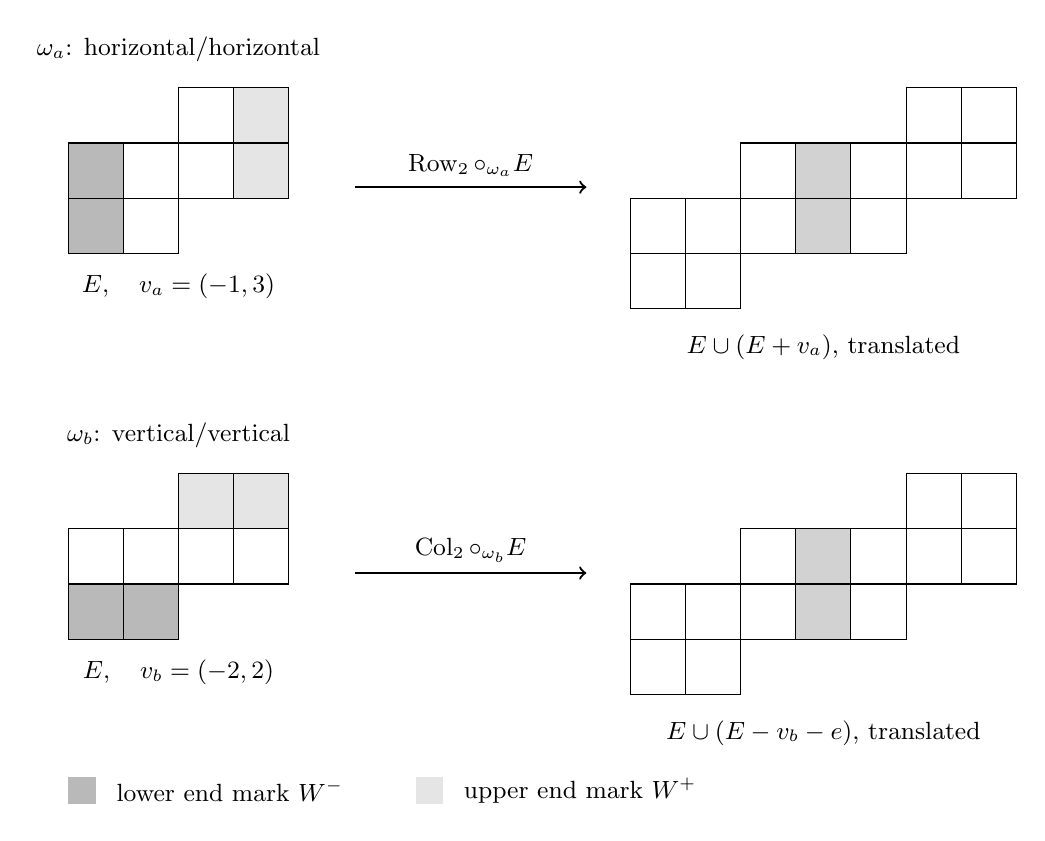
\begin{tikzpicture}[x=7mm,y=-7mm,font=\small]
 \begin{scope}
  \node at (2,-0.7) {\(\omega_a\): horizontal/horizontal};
  \foreach \i/\j in {1/0,2/0}
   \fill[gray!55] (\j,\i) rectangle +(1,1);
  \foreach \i/\j in {0/3,1/3}
   \fill[gray!20] (\j,\i) rectangle +(1,1);
  \foreach \i/\j in {0/2,0/3,1/0,1/1,1/2,1/3,2/0,2/1}
   \draw (\j,\i) rectangle +(1,1);
  \node at (2,3.6) {\(E,\quad v_a=(-1,3)\)};
  \draw[->,thick] (5.2,1.8) -- (9.4,1.8)
   node[midway,above] {\(\Row_2\circ_{\omega_a}E\)};
  \begin{scope}[shift={(10.2,0)}]
   \foreach \i/\j in {1/3,2/3}
    \fill[gray!35] (\j,\i) rectangle +(1,1);
   \foreach \i/\j in
    {0/5,0/6,1/2,1/3,1/4,1/5,1/6,
     2/0,2/1,2/2,2/3,2/4,3/0,3/1}
    \draw (\j,\i) rectangle +(1,1);
   \node at (3.5,4.7) {\(E\cup(E+v_a)\), translated};
  \end{scope}
 \end{scope}
 \begin{scope}[shift={(0,7)}]
  \node at (2,-0.7) {\(\omega_b\): vertical/vertical};
  \foreach \i/\j in {2/0,2/1}
   \fill[gray!55] (\j,\i) rectangle +(1,1);
  \foreach \i/\j in {0/2,0/3}
   \fill[gray!20] (\j,\i) rectangle +(1,1);
  \foreach \i/\j in {0/2,0/3,1/0,1/1,1/2,1/3,2/0,2/1}
   \draw (\j,\i) rectangle +(1,1);
  \node at (2,3.6) {\(E,\quad v_b=(-2,2)\)};
  \draw[->,thick] (5.2,1.8) -- (9.4,1.8)
   node[midway,above] {\(\Col_2\circ_{\omega_b}E\)};
  \begin{scope}[shift={(10.2,0)}]
   \foreach \i/\j in {1/3,2/3}
    \fill[gray!35] (\j,\i) rectangle +(1,1);
   \foreach \i/\j in
    {0/5,0/6,1/2,1/3,1/4,1/5,1/6,
     2/0,2/1,2/2,2/3,2/4,3/0,3/1}
    \draw (\j,\i) rectangle +(1,1);
   \node at (3.5,4.7) {\(E\cup(E-v_b-e)\), translated};
  \end{scope}
 \end{scope}
 \fill[gray!55] (0,12.5) rectangle +(0.5,0.5);
 \node[anchor=west] at (0.7,12.75) {lower end mark \(W^-\)};
 \fill[gray!20] (6.3,12.5) rectangle +(0.5,0.5);
 \node[anchor=west] at (7,12.75) {upper end mark \(W^+\)};
\end{tikzpicture}
\caption{Two full ordinary marks on \(E=(4,4,2)/(2)\), each of
width \(2\) and period \(4\), and their equal \(14\)-cell composites
after translation.  On each inner, dark and light cells are the
complete lower and upper marked copies; on each composite, shading
indicates the two cells shared by its placed copies of \(E\).
The gauge changes the outer function from \(h_2\) to
\(e_2=\ii(h_2)\ne h_2\).  This is a geometric I--IV example,
not an assertion of source minimality or scalar activity.}
\label{fig:ordinary-gauge}
\end{figure}

\subsection{The smaller-area package}

\begin{definition}\label{def:joint}
A diagram is rooted if it has a proper legal chart.  For every connected Schur class of occupied area less than \(n\), the hypothesis \(\Jlower\) asserts:
\begin{enumerate}
\item if one member is rooted, every member is rooted;
\item if the class contains two rotation orbits, some member is rooted;
\item any two rooted members have the same source-minimal marked key, modulo transported full-mark rotation and the gauge \eqref{eq:gauge}.
\end{enumerate}
The key consists of the full marked source-minimal inner together with the outer Schur function.  No current-area assertion is included.
\end{definition}

\begin{lemma}\label{lem:lower-full}
Assume \(\Jlower\), and let \(G\) be connected with \(|G|<n\).
Write \([G]\) for its connected Schur class.
\begin{enumerate}
\item If \(G\) has a prescribed source-minimal chart \(\chi=(A,K,\kappa)\), then \([G]=\mathcal F(\kappa,s_A)\).
\item If \(G\) is chartless, then \([G]=\{G,G^*\}\).
\item If \(G\) and a nonrotation mate have equal whole functions, then \(G\) has a proper source-minimal chart and the mate belongs to its prescribed full fiber.
\end{enumerate}
\end{lemma}
\begin{proof}
For (1), rootedness transfer makes every mate rooted, and key invariance, followed by source-minimal domination, gives membership in the prescribed fiber.  Forward sufficiency gives the reverse inclusion.  For (2), a second rotation orbit would give a rooted member by root existence, and then a root of \(G\) by transfer.  Part (3) follows by the same two assertions and then (1).  This is also the lower full-fiber consequence in \cite[Smaller-area full-fiber lemma]{Shields2026RibbonPeriod}.
\end{proof}

\begin{lemma}\label{lem:strict-area}
In a proper legal composition \(P=A\circ_\kappa K\), both factors have area strictly smaller than \(P\).  An actual connected child obtained by deleting a nonempty outer strip, or by one of the interior cuts used below, has smaller occupied area whenever it is a strict cell subset.  A Schur-equal mate of that child has the same strict area.
\end{lemma}
\begin{proof}
The extreme copy of \(K\) is contained in \(P\), and a second outer
diagonal contributes contents outside that copy, proving \(|K|<|P|\).
For the other factor, put
\(\alpha=|W|\), \(\beta=|\widehat W|\),
\(\gamma=|\widehat O|\).  The full modified-composition identity and
its generator-span normalization give
\[
 |K|=p+\alpha+\beta+\gamma,\qquad
 |P|=p|A|+\alpha r(A)+\beta c(A)+\gamma N_A.
\]
An ordinary gauge exchanges the indicated row and column conventions
together.  All three coefficients are nonnegative and a proper inner
has \(p\ge2\), so \(|P|\ge2|A|>|A|\).  These are the full all-type
identities, including the mixed supplements
\cite{OlsonHarris2024HopfApplications,Shields2026CornerDescent}.
A strict finite cell subset has smaller area.  Homogeneity of a skew
Schur function transfers the area equality to every mate.  We invoke this
lemma only after the actual cell object and its proper inclusion have
been established.
\end{proof}
\section{Factor readout and the two-copy reduction}\label{sec:reduction}

Apply \cite[Ribbon-outer period rigidity]{Shields2026RibbonPeriod} to
the original charts in \Cref{thm:recognition}.  It gives \(p=q\).
Throughout this section \(p\) denotes this common original period.
The span law gives equal widths and outer spans.  By corner transport,
a nonempty component of \(C^-\) would contribute a connected prime
of span at least \(p\) to the common corner, whereas the ribbon-outer
chart contributes only factors of span below \(p\).  Thus \(C\)
is a ribbon.  These uses require no current-area instance of
\(\Jlower\).

\subsection{Ordinary and mixed readout}

Put
\[
 \delta_k=p_k^\perp=\sum_{j\ge k}h_{j-k}\frac{\partial}{\partial h_j},\qquad
 \Vop_k=\sum_{j\ge1}j h_j\frac{\partial}{\partial h_{j+k}}.
\]
The two derivations have different roles.  In particular, \(\Vop_k h_k=0\), whereas \(\delta_k h_k=1\).  A mixed period-\(p\) chart has \(\delta_{kp}s_F=0\) for every \(k\ge1\): its complete fixed boundary word makes every shifted Jacobi--Trudi row either duplicate or zero.  A proper ordinary chart has \(\delta_p s_F\ne0\), by the ordinary readout theorem \cite[Factor recovery at a prescribed period and mixed-vanishing lemma]{Shields2026Readout}.  Thus the two original equal-period charts have the same ordinary or mixed category.  Empty marks belong to the ordinary category.

For a nonzero rational multiple of a skew Schur polynomial, \(\operatorname{prim}\) clears denominators, divides the integer content, and makes the coefficient of the minimum-square monomial positive.  The ordinary readout gives
\begin{equation}\label{rt:ordinary-readout}
 a=\max\{j:\delta_p^jP\ne0\}=|D|,\qquad
 s_E=\operatorname{prim}\left(
 \frac{\delta_p^{a-1}P}{\gcd(\delta_p^{a-1}P,\delta_p^aP)}\right),
\end{equation}
and the ratios \(\delta_{p\lambda}P/\delta_p^aP\), for \(\lambda\vdash a\), recover the complete outer character.  The recovered outer is \(s_D\) in case (a) and \(\ii(s_D)\) in case (b), exactly as required by \eqref{eq:gauge}.

For the mixed case, rotate the whole chart to case (d).  In the notation of the mixed weighted covariance and mixed ribbon factor recovery theorems of \cite{Shields2026Readout}, put
\[
 \rho=s-t,\quad A=s_W,\quad B=s_{\widehat W},\quad
 C_0=s_{\widehat O},\quad \chi=(-1)^{-v_1}ABC_0,\quad
 \mathcal B_k=p\Vop_k+\rho\delta_k,
\]
where \(0\le t<s\le w<p\).  The map is
\(\phi(h_j)=A^{j-1}s_{\Row_j\circ_\omega E}\) for \(j\ge1\), with \(\phi(1)=1\).
The following displayed specializations will also be used by the two-copy argument.  The weighted beta-move identity of \cite{Shields2026Readout} is
\begin{equation}\label{rt:weighted-moves}
 \Vop_r s_{X/Y}=
 \sum_{x\in X}(x-r)\det\JT_{X:x\mapsto x-r,Y}
 -\sum_{y\in Y}y\det\JT_{X,Y:y\mapsto y+r}.
\end{equation}
The lists remain in their original positions; subsequent sorting contributes its determinant sign, including at zero and negative entry indices.  For \(1\le k\le m\), the column move at \((m-k)p+s\) in the actual row power leaves
\begin{equation}\label{rt:strip-remainder}
 (\Row_{m-k}\circ_\omega E)\ \sqcup\!
 \bigsqcup_{j=m-k}^{m-1}(\widehat O+jv+e)
 \ \sqcup\!
 \bigsqcup_{j=m-k+1}^{m}(\widehat W+jv+e).
\end{equation}
This is the mixed strip remainder of \cite{Shields2026Readout}, with the first term interpreted as \(W\) at \(m=k\), not as the algebraic unit.  Its marked intervals have heights differing from those of \(\widehat W\) by one precisely on residues \(t,\ldots,s-1\).
For a homogeneous \(Q\) of weight \(m\), the mixed terminal evaluation of the same reference gives
\begin{equation}\label{rt:weighted-top}
 \mathcal B_1^mQ=m!p^m Q(1^{\rho/p}).
\end{equation}
It is nonzero when \(Q\) is a ribbon Schur function.  Thus the mixed ribbon inverse uses \(m=\max\{j:\Vop_p^jP\ne0\}\), the terminal quotient \(s_E/(\rho\chi)\), and the fixed-order triangular system for the outer character.

Applied to the two actual mixed charts in \eqref{eq:original-charts}, that inverse gives \(s_E=s_U\) and \(s_D=s_C\), with genuine outer functions.  In the ordinary case \eqref{rt:ordinary-readout} gives \(s_E=s_U\) and equality of the recovered outers in the indicated gauge.  Both inners have area less than \(n\), by \Cref{lem:strict-area}.

If \(U=E\) or \(E^*\), transport its full upper mark to \(E\).  The fixed-width atlas in \Cref{prop:gluing-inputs}(1) identifies the marks, with only the ordinary gauge as a possible double.  In the mixed case the mark is unique.  The recovered outer functions then give exactly \eqref{eq:main-fiber}.  A chartless \(E\) forces this case by \Cref{lem:lower-full}(2).

\subsection{Why the remaining original outer has two cells}
\begin{lemma}\label{rt:domino-probe}
If the original ribbon outer has at least three cells, then \Cref{thm:recognition} holds.  For a two-cell original outer, it also holds when the opposite domino probe is strictly smaller than the original parent.  In the mixed case only the row-two selector remains.
\end{lemma}
\begin{proof}
Use the composition covariance of \cite{Shields2026Readout} on the actual original chart.  For an ordinary mark put
\(A=s_W\), \(B=s_{\widehat W}\), \(C_0=s_{\widehat O}\), and let
\(\mathcal M_\omega(h_j)=A^{j-1}s_{\Row_j\circ_\omega E}\).
Its algebraic value on one is one.  In the read-outer convention,
\[
 (\Phi,Q)=
 \begin{cases}
  (\mathcal M_\omega,s_D),&\mathrm{(a)},\\
  (\mathcal M_\omega\circ\ii,\ii(s_D)),&\mathrm{(b)}.
 \end{cases}
\]
For \(a=|D|\), \(r_D=\operatorname{rows}D\), \(c_D=\operatorname{cols}D\), and \(M_D=N_D\), the entire ordinary normalization is
\[
 \Phi(Q)=A^{a-r_D}B^{a-c_D}C_0^{a-M_D}s_{D\circ_\omega E}.
\]
Write \(e=s_E\), \(\xi=\delta_p e\), and \(\theta=\Vop_pe/\xi\).  The cited covariance gives \(|\theta|<p\) and
\[
 \Vop_{kp}\Phi(f)=\xi^k\Phi((p\Vop_k+\theta\delta_k)f).
\]
In case (b), the coarse involution in \(\Phi\), the physical signs, and the whole normalizer are part of this identity.  At either genuine empty edge \(\theta=0\).  For a mixed chart use the positive-phase convention above, with \(\theta=\rho\), \(\Phi=\phi\), \(Q=s_D\), and \(\xi\) replaced by \(\chi\).  Its full modifier has the ribbon sign \((-1)^{r_D-1}\), retained below in \(\mathcal N_D\).

Let \(Q\) be the read outer function in this convention, and let \(m=|D|\ge3\).  Write
\[
 (p\Vop_{m-2}+\theta\delta_{m-2})Q=\gamma p_2+\lambda p_1^2.
\]
Let \(\chi_Q\) be the skew character with Frobenius characteristic
\(Q\).  Its \(p_2\)-coefficient is
\[
 \gamma=p\chi_Q(m)+\frac{\theta}{2}\chi_Q(m-2,2)\ne0.
\]
The read ribbon is \(D\) or \(\AT(D)\), according to the displayed
convention.  If it has \(l\) rows, then \(\chi_Q(m)=(-1)^{l-1}\).
Its interval-coarsening expansion gives
\[
 \chi_Q(m-2,2)=(-1)^{l-1}
 \bigl(1-\one_{2\text{ a proper partial sum}}
          -\one_{m-2\text{ a proper partial sum}}\bigr).
\]
The occurrences are counted separately at \(m=4\).  Its absolute value is at most one, so \(|\theta|<p\) proves nonvanishing, also at \(m=3\).

Retain \(A=s_W\) and \(B=s_{\widehat W}\) for the actual current mark.
Let \(\zeta\) denote \(\xi\) or \(\chi\), and write the complete composition
normalization as \(\Phi(Q)=\mathcal N_D P\).
The scalar-normalization factor \(S=\zeta^m/\mathcal N_D\) is read by
\[
 S=\frac{\delta_p^m P}{\delta_1^m Q}\quad\hbox{in the ordinary case},
 \qquad
 S=\frac{\Vop_p^m P}{(p\Vop_1+\rho\delta_1)^m Q}
       \quad\hbox{in the mixed case}.
\]
The ordinary denominator is the positive number of standard tableaux
of the ribbon, and the mixed denominator is nonzero by
\eqref{rt:weighted-top}.  Hence
\begin{equation}\label{rt:domino-readout}
 \zeta^2\Vop_{(m-2)p}P/S=\gamma\Phi(p_2)+\lambda e^2
\end{equation}
reads \(\Phi(p_2)\).  Newton's identity reads \(\Phi(h_2)\) and \(\Phi(e_2)\).  In case (a), these are \(A s_{\Row_2\circ E}\) and \(B s_{\Col_2\circ E}\); case (b) swaps their assignments.  In case (d), they are
\[
 A s_{\Row_2\circ E},\qquad -B s_{\Col_2\circ E}.
\]
The minus sign is the column-domino specialization of the full mixed modifier in \cite[Mixed weighted covariance]{Shields2026Readout}.  Each expression has a unique connected prime factor of span greater than \(p\), namely the actual domino probe of span \(2p+w\).  Thus both original parents read the same two probe functions.

Choose a domino contained in \(D\).  Its composition is a translated strict cell subset of \(F\).  For ordinary marks this is immediate from the affine origins \eqref{eq:copy-origins}.  For mixed marks, a ribbon has one cell on each diagonal, so the rank correction in \eqref{eq:copy-origins} vanishes; the supplemental mark of a contained vertical pair is exactly the one present in the whole composite.  The probe has smaller span and hence is a strict subset.  Its mate has the same smaller area.  Since \(E\) is not a line, outer-independent minimality makes the displayed probe chart source-minimal.  Lower full-fiber transport now puts the mate probe in its prescribed fiber.  The mate has two actual period-\(p\) charts, so same-parent equal-period comparison identifies the full marked inners up to the permitted gauge and rotation.  The recovered outer functions give \eqref{eq:main-fiber}.

At \(m=2\), \eqref{rt:domino-readout} would require a zero-index operator, which gives no smaller probe.  Instead the recovered outer and terminal derivative determine \(\mathcal N_D\); Newton's identity then reads the opposite domino.  It may be used for descent exactly when it is strictly smaller.  The ordinary domino areas are \(2|E|-|W|\) and \(2|E|-|\widehat W|\).  In the mixed case, the marked intervals in \eqref{rt:strip-remainder} give \(|W|-|\widehat W|=s-t>0\).  Hence the mixed column-two parent is strictly larger than its row-two probe and is discharged.  Only the mixed row-two selector remains.
\end{proof}

\subsection{The actual common finer source}

\begin{proposition}\label{rt:lower-landing}
Under the hypotheses of \Cref{thm:recognition}, either the prescribed-fiber conclusion already holds, or, after a permitted whole rotation, there are actual proper source-minimal charts
\begin{equation}\label{rt:common-finer}
 E=V\circ_\mu J,\qquad U=V'\circ_\mu J,\qquad s_V=s_{V'},
\end{equation}
with the same literal connected inner \(J\) and the same full legal mark \(\mu\).  The minimum is held on \(E\) and transported to \(U\); no minimum is imposed on \(J\).
\end{proposition}
\begin{proof}
The literal and rotation cases were settled before \Cref{rt:domino-probe}.  Otherwise the lower class has at least two rotation orbits.  Root existence and rootedness transfer make \(E\) rooted.  Choose a genuine source-minimal proper chart \(E=V\circ_\mu J\).  The full-fiber consequence \Cref{lem:lower-full}(1) gives a chart of \(U\) with equal genuine outer function and with marked inner \(\mu\) or its transported rotation.  In the latter case rotate the entire original chart of \(H\), including its upper mark and supplements.  This gives \eqref{rt:common-finer}; the target fiber is rotation-stable, so the final conclusion transports back.  Lower key invariance identifies the source-minimal score on \(U\).  The construction uses only classes of area \(|E|<n\).
\end{proof}

\subsection{The remaining geometric domain}

At the nonliteral landing \eqref{rt:common-finer}, put
\begin{equation}\label{rt:finer-parameters}
 N_J=r+v,\qquad N_V=N_{V'}=M,\qquad
 S=N_E=N_U=Mr+v,\qquad Q=S-w.
\end{equation}
Here \(r,v\) are the finer period and width, and \(Q\) is the original upper period.  In particular, \(Q\) is not a stationary exponent.  If \(V=V'\), then \(E=U\) and the direct fiber argument applies.  Equal coarse functions with \(M\le2\), or with a line as one realization, force literal equality.  Thus every remaining finite comparison has \(M\ge3\) and nonline coarse outers.

\begin{proposition}\label{rt:preprocessing}
At \eqref{rt:common-finer}, the theorem is reduced to
\begin{equation}\label{rt:narrow-domain}
 J\text{ nonline},\qquad 0\le w<r,\qquad w\ne v,
\end{equation}
with the same actual full upper mark and the same actual domino selector on \(E,U\).  The proof includes the empty-width case and the original selector and gauge.  Every excluded case either already gives the prescribed fiber or constructs an actual proper chart of a held source or original parent with strictly smaller score.
\end{proposition}
\begin{proof}
If \(r\mid Q\), apply the complete aligned theorem to the actual finer chart and the actual upper mark.  It gives a proper period-\(r\) chart of the original parent.  Since \(Q>w\), \(M\ge3\), and \(w\equiv v\pmod r\), its score \((v,r+v)\) is strictly below \((w,Q+w)\).  This contradicts the original source minimum.

The wide case \(w>r\), the boundary case \(w=r\), and the literal line-finer case are proved in \Cref{rt:wide,rt:boundary,rt:line-finer}.  Their source constructions precede every comparison of scores.  They leave \eqref{rt:narrow-domain}; the equality \(w=v\) is already aligned.

For \(0<w<r\), the first and last \(r\) source windows in \eqref{rt:common-finer} come from the same literal \(J\).  Their final-copy origins agree: in the ordinary cases the origin also reads the equal coarse row count, and in the mixed cases it is \((M-1)v_\mu\).  Supplements do not enter these extreme windows.  The complete windows \([0,w]\) and \([S-w-1,S-1]\) therefore agree as cell sets, and \(2w<S\).  The mark-locality lemma \cite[Locality of legal marks in the two end windows]{Shields2026Gluing} transfers the full upper mark, including both hatted clauses at every integer translate.  The fixed-width atlas permits only the ordinary double; applying its genuine gauge also changes the actual upper domino.

After this transfer the selectors agree.  If the source has \(t_E\) rows and the mark \(a\) rows, put \(d=t_E-a\).  The row-two parent has \(t_E+d\) rows.  An ordinary(a) column-two parent has \(t_E+d+1\); an ordinary(b) one has \(t_E+|d-1|\).  Both differ from the row count of the row-two parent, including \(d=0\).  In a mixed upper, the column-two parent has the same two copies as the row-two parent and a strictly positive supplemental patch.  The patch is determined by the common two end windows, so its area is the same on both sources.  Equal whole functions thus force the same selector by row count in the ordinary cases and by area in the mixed cases.  At \(w=0\), use the actual horizontal edges: the two selectors have different row counts, and converting a vertical edge applies \eqref{eq:gauge}.  No positive-width argument is used for this empty case.
\end{proof}

The remaining ordinary and empty comparisons must yield full marked
reflection or an improving aligned source chart; their gcd-one
certificates retain the actual ordinary positive, empty-upper, or mixed
sign endpoint alternatives.  A mixed comparison must instead give a
literal or whole-parent fiber finish, or a legal divisor alignable
through the held source charts.  Only a private active mixed second
response requires stationary separation.

\section{Finite comparisons on actual composition charts}\label{sec:comparison}

The reduction leaves two actual compositions through the same full marked
inner,
\begin{equation}\label{ph:landing}
 E=V\circ_\mu J,\qquad U=V'\circ_\mu J,\qquad
 s_V=s_{V'},\qquad V\ne V',
\end{equation}
where the displayed chart of \(E\) is source-minimal.  Write
\[
 \begin{aligned}
 N_J&=r+v,\qquad N_V=N_{V'}=M\ge3,\\
 S&=N_E=N_U=Mr+v,\qquad Q=S-w=Mr+\delta,\quad \delta=v-w.
 \end{aligned}
\]
The original upper width satisfies \(0\le w<r\), \(w\ne v\).
This section extracts information from the actual whole-parent comparison.
In particular, the span \(M\) of the finite algebra below is supplied by
\(V\); it is not replaced by a smaller test outer.

\subsection{A complete raised current}
For a connected source with full Jacobi--Trudi matrix \(A=(h_{x-y})\), set
\[
 e=\det A,\qquad \kappa=\partial_{h_S}e,\qquad
 K_Q=(h_{Q+x-y}),\qquad T_Q(A)=\operatorname{tr}(\operatorname{adj}(A)K_Q).
\]
The raised matrix includes entries that were negative-index zeros in \(A\).
A raised index zero is the actual unit \(h_0=1\).
Let \(\mathcal G_Q=(\operatorname{adj}(A)K_Q\operatorname{adj}(A))_{0,S}\),
with the indicated entry indexed by its actual column and row.

\begin{lemma}\label{ph:activation}
At the matched narrow upper comparison in \eqref{ph:landing}, the actual
whole-parent equality supplies
\begin{equation}\label{ph:current}
 T_Q(E)=T_Q(U).
\end{equation}
Both sources also satisfy the open mate implications
\begin{equation}\label{ph:UM}
 \begin{aligned}
 x\in X_E,\quad0<x<w&\ \Longrightarrow\ Q+x\in X_E,\\
 y\in Y_E,\quad Q<y<S&\ \Longrightarrow\ y-Q\in Y_E,
 \end{aligned}
\end{equation}
and the corresponding implications on \(U\).  The assertion holds for
all four positive upper attachment types, and for the genuine ordinary
empty upper when the finer is ordinary or empty.  A mixed finer with
an empty upper is already disposed of by \Cref{rt:mixed-empty}.
\end{lemma}
\begin{proof}
Form the actual two-copy diagram \(\Row_2\circ_\omega E\).
Its first and last \(Q\) diagonals are the actual end windows of \(E\).
The complete coding table changes initial to terminal bits only as follows:
\[
\begin{array}{c|cc}
 &\text{column changes}&\text{row changes}\\ \hline
(a)&t:1\longmapsto0&s:0\longmapsto1\\
(b)&s:1\longmapsto0&t:0\longmapsto1\\
(c)&\text{none}&t,s:0\longmapsto1\\
(d)&t,s:1\longmapsto0&\text{none}.
\end{array}
\]
A low row is never lost and a high column is never new, giving
\eqref{ph:UM}, including endpoint contacts by the strict displayed ranges.
This uses the actual supplemented composition formula; it is not an
implication of a height word alone.

For a positive ordinary upper, \Cref{ph:ordinary-activation} gives the
whole \(\mathcal G_Q\) comparison.  At an empty ordinary upper the
row-mark splice in \Cref{ph:rectangular-splice} gives that comparison
directly.  In the vertical reading, the complete structured dual identity
\Cref{ph:structured-dual} retains the two
additional terms of the inverse-alphabet expansion:
\[
 \sum_{0<x<w}L_x(HR)_{Q+x},\qquad
 \sum_{Q<y<S}R_y(HL)_{S+Q-y}.
\]
Here \(L,R\) are the complete global null records.  The actual mate
implications make each numerator in these sums a source null equation;
thus both sums vanish.  The remaining sign is \((-1)^{w+1}\), common
on the matched pair.  This proves the same raw \(\mathcal G_Q\)
comparison in both ordinary readings, while rebuilding both fields.

For a mixed upper, the complete compound expansion is proved in
\Cref{ph:mixed-compound}.  If \(K_t\) is the actual top-row/returned-column
deletion, it gives
\begin{equation}\label{ph:compound-use}
 k_tT_Q(A)-eT_Q(K_t)=(-1)^{a+b}\,b_t\,s_{\Row_2\circ_\omega E},
\end{equation}
where \(a,b\) are the actual upper mark and private ranks.
For that upper overlap \(W\), of width \(w\), put
\(b_t=\det\JT(X_W\setminus\{w\},Y_W\setminus\{t\})\ne0\),
with both lists decreasing.  This is the unsigned proper mark minor
of \Cref{ph:mixed-compound}.  The complete corner has factorization
\(k_t=b_t n\widehat A\), with the entire private determinant \(n\).
The common top coefficient of \(e\), together with the common end data,
fixes \(n\); hence \(k_t\) is common.  Its connected factors have smaller
weight than \(e\).  Subtraction of \eqref{ph:compound-use} and connected
primality give \(e\mid\Delta T_Q\).  A complete current has ordinary
moment degree at most the number of source rows, equal to the ordinary
degree of \(e\).  Its surplus weight is \(Q>0\), so the quotient must
be zero.  Whole rotation proves the other mixed reading.

For completeness, the same degree argument converts the ordinary
\(\mathcal G_Q\) comparison into \eqref{ph:current}.  Differentiate the
entire adjugate, including the variation of \(K_Q\), to obtain
\begin{equation}\label{ph:jacobi-current}
 \mathcal G_Q=\kappa T_Q-e\,\partial_{h_S}T_Q+e\,U_w(e),\qquad
 U_w(e)=
 \begin{cases}
 \partial_{h_w}e,&w>0,\\
 n_Ee-\sum_{d>0}h_d\partial_{h_d}e,&w=0,
 \end{cases}
\end{equation}
For \(w>0\) the derivative is at a genuine positive index.
For \(w=0\), \(n_E\) is the actual row rank and the displayed expression
is the entire unit-cofactor sum, earned by homogeneous Euler identity.
The common whole function and row rank make this term common.
Subtraction gives
\(\kappa\Delta T_Q=e\partial_{h_S}\Delta T_Q\).
The connected polynomial \(e\) is prime and coprime to its proper corner
\(\kappa\); the preceding degree and weight argument again gives zero.
No individual cofactor summand has been observed separately.
\end{proof}

\subsection{The two actual returned coordinates}
Normalize an ordinary finer to case \((a)\) by the whole-chart
transport of \Cref{rt:transports}.  For an original case \((b)\)
comparison, transport both sources and their complete upper
presentations first, rebuild the fields, and apply
\Cref{ph:activation} on those image charts.
The current and global scalar are thereby earned in the normalized
field, not identified with an unmarked bare antitranspose scalar.
If the finer contacts are \(s,t\),
its complete flags are
\begin{equation}\label{ph:ordinary-flags}
 \begin{aligned}
 X_J&=(r+X_W)\sqcup B_-\sqcup(X_W\setminus\{s\}),\\
 Y_J&=(r+(Y_W\setminus\{t\}))\sqcup C_-\sqcup Y_W,
 \end{aligned}
\end{equation}
where \(B_-,C_-\subset(v,r)\).  Its returned coordinate is a
\emph{numerator} coefficient.  In the actual normalized rational chart,
\[
 H=P'/G',\qquad G'_t=1,\qquad P'_s=R_0.
\]
The outside coordinates are precisely the available \(P'_i\) and \(G'_j\)
with \(v<i,j<N_J\); a numerator coordinate is available at a missing row,
and a denominator coordinate at a present column.

For mixed case \((d)\), with \(0\le t<s\le v\), the full flags are
\begin{equation}\label{ph:mixed-flags}
 \begin{aligned}
 X_J&=X_W\sqcup B_-\sqcup(r+X_W),\\
 Y_J&=(Y_W\cup\{s\})\sqcup C_-\sqcup(r+(Y_W\setminus\{t\})).
 \end{aligned}
\end{equation}
The returned coordinate is now a \emph{denominator} coefficient:
\[
 G'_t=1,\qquad G'_s=-R_0,\qquad
 R_0=(-1)^{|Y_W\cap(t,s)|}\frac{s_W}{\det\JT(X_W,(Y_W\setminus\{t\})\cup\{s\})}.
\]
Its coherent degree is zero and its weight is \(\rho=s-t>0\).
This distinction explains why the ordinary finite argument does not kill
the mixed stationary responses by homogeneity alone.

\begin{lemma}\label{ph:source-chart}
For each of these two cases, the returned coefficients
\(R_1,\ldots,R_M\), all genuine outside high coefficients at depths
\(1,\ldots,M-1\), and the complete neutral fine coordinates give a rational
coordinate chart of the actual whole source field.  All returned
coefficients remain fixed when an outside coefficient is varied.
\end{lemma}
\begin{proof}
Write \(R(u)=\sum_{j=0}^MR_ju^j\).  For an ordinary finer use
\begin{equation}\label{ph:ordinary-source-chart}
 \begin{aligned}
 P_{\rm full}&=P'+z^s(R(z^r)-R_0)
       +\sum_{a,i}\alpha_{a,i}z^{(M-a)r+i},\\
 G_{\rm full}&=G'+\sum_{a,j}\beta_{a,j}z^{(M-a)r+j},
 \qquad H_{\rm full}=P_{\rm full}/G_{\rm full}.
 \end{aligned}
\end{equation}
For a mixed finer replace these first two lines by
\begin{equation}\label{ph:mixed-source-chart}
 P_{\rm full}=P'+\sum_{a,i}\alpha_{a,i}z^{(M-a)r+i},\qquad
 G_{\rm full}=G'-z^s(R(z^r)-R_0)
                  +\sum_{a,j}\beta_{a,j}z^{(M-a)r+j}.
\end{equation}
Every outside wave has its actual label strictly between \(N_J\) and
\(S\).  In the ordinary case, the source-clipped records
\(z^{kr}G_{\rm full}\) annihilate every fixed row and return
\(R_{j-k}\) at the actual returned row.  The full fixed-word solve
therefore recovers exactly these coefficients.  Conversely it recovers
\(G_{\rm full}\), and multiplication by \(H_{\rm full}\) recovers all
available numerator coefficients.  This is an inverse rational map.

For the mixed case use the square baseline containing every fixed column
and all columns \(jr+s\), \(0\le j\le M\).  Its determinant is
\begin{equation}\label{ph:mixed-baseline-det}
 \widehat A^{M+1}C_{\rm priv}^{M},\qquad
 \widehat A=\det\JT(X_W,(Y_W\setminus\{t\})\cup\{s\}),\quad
 C_{\rm priv}=\det\JT(B_-,C_-).
\end{equation}
Both factors are nonzero weak skew determinants; empty blocks have
determinant one.  Its actual inverse sends the column \(kr+t\) to the
\(jr+s\) coefficient \(R_{j-k}\).  The final partial mark block gives
this coefficient also at \(j=M\): its constant inverse row has no private
part.  Complementary-column expansion thus gives the complete coarse
Toeplitz determinant, with the actual sorting sign.  Equality of the
source and coarse functions fixes this sign on the two sources.
The inverse solve recovers the whole denominator null record and all its
outside coefficients.  Before recovering the neutral seed, add back
\(z^s(R(z^r)-R_0)\).  This is necessary when the \(R_1\) term occurs at
\(r+s<N_J\).  It cannot be confused with an outside denominator coordinate,
since \(r+s\) is absent from the actual finer column list.
These solves prove the assertion on the nonempty open set where the
complete fixed determinants and the normalizing coefficients are nonzero.
\end{proof}

For an empty finer, the actual chart is different:
\begin{equation}\label{ph:empty-chart}
 \begin{aligned}
 G_0&=1,\qquad P_0=R_0=\nu,\\
 P_{\rm full}&=P+\sum_{j=1}^MR_jz^{jr}
                  +\sum\alpha_{a,i}z^{(M-a)r+i},\\
 G_{\rm full}&=G+\sum\beta_{a,j}z^{(M-a)r+j}.
 \end{aligned}
\end{equation}
There is one coherent unit, and \(P_r=R_1\) is returned.  The proper
fixed matrix has \(M\) copies of the full proper corner of \(J\), including
all crossing blocks.  The same direct and inverse solve proves
\eqref{ph:empty-chart}; no outside derivative of \(P_r\) is used.

\subsection{Why two finite waves suffice}
Let \(\mathcal A_V(j,k)\) be the complete keyed coarse adjugate, zero at
absent flags, and let \(\Delta\mathcal A=\mathcal A_V-\mathcal A_{V'}\).
A Schur-complement differentiation of the entire source gives
\begin{equation}\label{ph:effective-current}
 \sum_{j,k}\Delta\mathcal A(j,k)(WK_QU)_{j,k}=0,
 \qquad W=(I,-BD^{-1}),\quad U=\binom{I}{-D^{-1}C}.
\end{equation}
The common fixed trace is multiplied by the common entire coarse
determinant and cancels as a whole.  The fixed block \(D\) retains both
partial end blocks and all private factors.

Here are the response series used in \eqref{ph:effective-current}.  Put
\(\mathcal H_d(u)=\sum_{n\ge0}h_{nr+d}u^n\).
For an ordinary finer let
\[
 D(u)=(\mathcal H_{b-c}(u))_{b\in B_0,c\in C_0},\quad
 L=\mathcal H_{s-C_0}D^{-1},\quad
 \Theta_d=\mathcal H_{s-d}-L\mathcal H_{B_0-d},
\]
where \(B_0=(X_W\setminus\{s\})\sqcup B_-\) and
\(C_0=(Y_W\setminus\{t\})\sqcup C_-\).
Set \(\Lambda_b=L_b\) at an actual fixed row, \(\Lambda_s=-1\), and
zero at absent rows.  Extend by \(\Lambda_{b+r}=u\Lambda_b\).
The responses are
\[
 F_{P_i}=\Lambda_{i-\delta},\qquad F_{G_j}=\Theta_{j-\delta}.
\]
For mixed \((d)\), use
\[
 D_s(u)=(\mathcal H_{b-c})_{b\in X_W\sqcup B_-,
 c\in(Y_W\setminus\{t\})\sqcup C_-\sqcup\{s\}},\quad
 \ell=e_s^TD_s^{-1},\quad\Theta_d=\ell\mathcal H_{(X_W\sqcup B_-)-d},
\]
and
\[
 F_{P_i}=\ell_{i-\delta},\qquad F_{G_j}=-\Theta_{j-\delta}.
\]
The exact distinguished values are
\(\Theta_c=0\) on fixed columns, \(\Theta_s=1\), and
\(\Theta_t=R(u)\).  At an empty finer take the ordinary formulas with
actual returned phase zero and its independently constructed chart
\eqref{ph:empty-chart}.

\begin{proposition}\label{ph:finite-block}
At the actual comparison above, write \(F_n=[u^n]F\).  At the supplied
\(M\),
\begin{equation}\label{ph:killing}
 F_M=0,\qquad \partial_xF_n=0\ (2\le n<M),\qquad
 F_1=A x+b,\quad A^T=-A,
\end{equation}
where \(x\) lists every outside coordinate.  For a positive ordinary
finer all coefficients of \(A,b\), and all stationary responses, depend
only on the actual returned clock.  The ordinary and empty cases satisfy
\(F_2=\cdots=F_M=0\).  For a mixed finer,
\begin{equation}\label{ph:mixed-finite}
 F_{n,P}=0\ (1\le n\le M),\qquad
 F_{1,G}=A_{GG}(R_0)x_G+b_1(R_0),\quad
 F_{n,G}=b_n(R_0)\ (2\le n<M).
\end{equation}
The assertion is obtained independently in both own fields: each is the
full rational coordinate field rebuilt from that chart's complete
source matrix and returned normalization.  Equal whole functions do
not identify their pivots or inverse matrices.
\end{proposition}
\begin{proof}
The neutral primitive numerator contributes to a raised record only at
\(k=M-1\) and \(0<x<w\).  Its index is \(r+\delta+x\).
The actual mate implication makes this a proper finer row, either in the
last private band or in the upper mark band; its numerator coefficient
is zero.  This proves neutral cancellation for both signs of \(\delta\).

On the simultaneous high-wave chart, a numerator pulse of cutoff \(a\)
meets row \((k-a)r+i-\delta\).  Its exact prefix is \(k\ge a\).
An apparent wrapped row at \(k=a-1\) would have phase \(b<w\);
\eqref{ph:UM} would force the input \(i\) to be a present finer row,
contrary to its availability.  In the ordinary returned phase it is the
absent coarse row zero; in the mixed phase the actual repeated row word
makes the same contradiction.  A denominator pulse lies beyond the source
exactly for \(k\ge a\) and gives the complete omitted-column residual.
Thus the live crossing is
\[
 -\sum_{a,i}\alpha_{a,i}[k\ge a]F_{j-k+a,i},
\]
up to the single consistent choice of response sign.  Every inverse is
computed after the pulses are inserted.

Scale all positive coarse returns by an auxiliary parameter.  Let \(\mu\)
be the first nonzero grade of the \emph{entire} array
\(\Delta\mathcal A\).  \Cref{ph:first-grade} proves that, at that same
grade, there is \(d\ge\lceil M/2\rceil\), \(a_0=M-d\), for which
\[
 C_{1,d}=C_{a_0,d}\ne0,\qquad C_{a,d}=0\quad(a>a_0),\qquad
 C_{a,D}=-\sum_{j-k=D,k\ge a}\Delta\mathcal A^{[\mu]}(j,k).
\]
All higher source corrections multiply a lower entire zero array.
Taking one or two actual waves and then separating genuine coarse weights
gives
\begin{align}
 C_{a,D}F_{D+a,i}&=0,\label{ph:one}\\
 C_{a,D}\partial_jF_{n,i}+C_{b,D}\partial_iF_{n,j}&=0,
 \qquad n=D+a+b-M.\label{ph:two}
\end{align}
The second equation contains both pulse assignments and the variation of
the inverse against the old crossing.  The high variation is exactly
\(u^{M-b}\) times the complete fine variation, by
\(dD^{-1}=-D^{-1}(dD)D^{-1}\).

Use \eqref{ph:one} at \(a_0\) to obtain \(F_M=0\).
For \(2\le n\le d\), use \eqref{ph:two} at
\((a,b)=(a_0+n-1,1)\); for \(d<n<M\), use \((n,a_0)\).
The first coefficient is zero and the second nonzero, giving outside
constancy.  The choice \((a_0,1)\) gives the Killing equation.
Differentiating its three cyclic versions gives all second derivatives
zero in characteristic zero, hence \eqref{ph:killing}.

Every nonreturned positive low coordinate has its actual high mate and
\(\partial_{\rm low}F_n=\partial_{\rm high}F_{n+1}\).
At zero, if \(t>0\), varying \(G'_0\) also varies
\(P'_0=\nu G'_0\), giving the combined high derivative
\(\partial_{G'_r}+\nu\partial_{P'_r}\).
Homogenizing the \emph{whole} equal-rank source identity gives the true
coherent-unit alias
\(\partial_\nu F_n=G'_0\partial_{P'_r}F_{n+1}\).
For \(t=0\), \(G'_0=1\) is fixed and only the latter alias is used.
For positive ordinary finers, descent from \(F_M=0\) leaves each
stationary coefficient a function of \(R_0\).  Its coherent degree makes
its \(P\) part constant and its \(G\) part proportional to \(R_0\).
Its actual weight \(nr+s+\delta-i\), \(n\ge2\), exceeds \(s\),
whereas the two possible weights are zero and \(s-t\); hence it vanishes.
For empty finers the outside coordinates already exhaust the fine field
over the single weight-zero unit \(\nu\), and the positive weight
\(nr-w-i\) gives the same conclusion without an alias of \(P_r\).

For mixed finers the stationary responses are outside-constant before
using these aliases, so all their nonreturned mark derivatives vanish.
The same holds for the coefficients of \(F_1\).  The mixed clock has
coherent degree zero, while a numerator response has degree \(-1\);
therefore every positive-order numerator response vanishes.  The
remaining \(GG\) coefficients and stationary values are rational
functions of \(R_0\), as asserted.  The generic endpoint is \(F_M=0\),
so at \(M=3\) it is \(F_3=0\).  No coefficient beyond the original
horizon has been used.
\end{proof}

\subsection{The ordinary and mixed first responses}
The finite block is not yet a geometric equality.  Its exact further
outputs are collected here; the complete algebra is in
\Cref{ph:gradient,ph:matrix-powers,ph:intercept-exclusion}.
The first-response matrix is the matrix \(A\) of \eqref{ph:killing}:
\[
 A_{\alpha\beta}=\partial_{x_\beta}[u]F_\alpha(u).
\]
Its rows and columns have the same outside-coordinate labels:
\(P'_i\) at missing rows \(v<i<N_J\), and \(G'_j\) at present
columns \(v<j<N_J\).  The response vector is the one defined after
\eqref{ph:effective-current}, in that chart's own normalized rational
field.  All returned and remaining neutral coordinates are held fixed;
the complete inverse matrices are differentiated.  At an empty finer
use the unprimed coordinates of \eqref{ph:empty-chart}.
An \emph{active pair} means a nonzero entry of the relevant \(PG\) or
\(GG\) first-response matrix, not merely a present coordinate or a
nonzero intercept.  A private fine index lies in \((v,r)\).
For an ordinary pair the inputs and their opposite-chart inputs must
lie in that band, with targets \(i-\delta,j-\delta\) checked separately.
For the mixed second response, the full condition is
\(v<j,k,j-\delta,k-\delta<r\), as in \eqref{ph:private-two}.


\begin{proposition}\label{ph:first-response}
At the actual narrow ordinary or empty finer comparison, the first matrix
is a constant pure \(PG\) skew matrix in each own returned chart.
All genuine returned intercepts remain.  At negative \(\delta\), and at
an empty finer, every active pair has four private inputs.
In the principal ordinary range, \Cref{ph:active-dichotomy} gives the
complete terminal-or-private alternative, including the actual head
and transpose checks.

At a positive mixed finer the entire \(GG\) matrix is constant.  If it is
nonzero, the actual coarse diagrams satisfy \(V'=V^*\), and every active
first row is free of its unwanted intercept.  For an active pair \(j,k\),
\begin{equation}\label{ph:CF0}
 j+k=r+s+t+\delta,\qquad
 \eta Q_{k+\epsilon}=cG_k/g_t,\qquad
 \eta Q_{j+\epsilon}=-cG_j/g_t,\qquad \epsilon=v-s-t.
\end{equation}
The constants and all proper factors are in their own fields.  Complete
coface factorization gives two actual connected equal-child pairs and two
complete component-product equalities, with their sorting signs and
multiplicities.  The entire-zero-matrix case has its separate native-word
conclusion in \Cref{ph:zero-matrix}; it does not require \(V'=V^*\).
\end{proposition}
\begin{proof}
For an ordinary finer, substitute the full moving returned series in the
one-wave equation and take its outside curl.  The exact equations are
\(H_aC_{PP}=0\), \(J_aC_{GG}=0\), together with
\(K_aC_{PG}=0\) when the coarse pair has not yet been reflected.
\Cref{ph:gradient} proves that the \(J\) family is nonzero, and either
the \(K\) family is nonzero, when the opposite own field excludes \(PP\),
or every \(K\) vanishes, when the same-cap and linearized same-cap
arguments make \(H_2\ne0\).  Thus the first matrix is pure \(PG\).
The actual zero-order vector is zero at negative \(\delta\) and at
empty width; its genuine low aliases remove every terminal active input.

For a mixed finer, two actual wave depths first give the whole ordered
sum, and the actual curl gives the whole product, of the two endpoint
polynomials.  The full own-atlas argument in \Cref{ph:matrix-powers}
excludes every nonconstant clock power in a matrix entry.  At power zero,
the crossed factor assignment is exactly the actual coarse rotation.
The full uncurled first-response equation then gives the finite Leibniz
defect of \Cref{ph:intercept-exclusion}.  Its positive-power exclusion
removes the unwanted active intercepts.  The permitted constant and
linear returned terms are not active: their putative partners would be
fixed low returns.  The actual one-period inverse row gives
\eqref{ph:CF0}.  Clearing its full prefix and suffix denominators and
using connected primality identifies the largest connected numerators,
then the remaining \emph{complete} products.  The two equations give
opposite actual signs.  The physical form and area inequalities are
recorded in \Cref{ph:coface-data}.
\end{proof}

\subsection{The remaining mixed stationary response}
The mixed first matrix may be nonzero.  Its active pairs supply the
physical child comparison, while a second response is still retained.
The complete finite identity now provides precisely the input to
whole-field stationary descent \cite{Shields2026Coframes}.

We use the complete coframes of \cite{Shields2026Coframes} in the actual
coarse alphabet.  For a board with full lists
\(X=\{M\}\cup I\), \(Y=S\cup\{0\}\), put
\[
 T=(H_{i-s})_{i\in I,s\in S},\qquad
 G=1-\sum_{s\in S}(T^{-1}(H_i)_{i\in I})_s z^s.
\]
All zero-index entries are the same returned clock
\(H_0=\vartheta=R_0\); negative indices are zero.  The inverse is taken
in the whole rational field, with every unit and crossing retained.
The empty proper matrix gives \(G=1\).  The left coframe \(C\) is the
right coframe of the normalized rotation in that same alphabet.
For these application coordinates write
\begin{equation}\label{ph:coframe-operator}
 \mathcal T_{G,C}(u)=G[uC]_{<M}-C[uG]_{<M},\qquad
 D=\mathcal T_{G,C}(H).
\end{equation}
The signed proper corner is the actual coefficient of the top letter,
so the complete whole determinant is \(\kappa[HG]_M\).
The coequal-data lemma of \cite{Shields2026Coframes} gives
\(\ord_zD\ge M+1\), \(\deg_zD\le2M-2\), and \(D\ne0\) for a distinct
pair.  Here \(M\) is the supplied coarse span, never a smaller test
span.  The whole returned series may retain its higher coefficients:
they do not affect the clipped terms or the required finite horizon.

\begin{proposition}\label{ph:stationary-packet}
On the nonzero mixed branch, let \(V'=V^*\), and let \(f\) be any actually
supplied active second response.  Write \(\vartheta=R_0\) for the
actual returned clock and \(H=\vartheta+\sum_{i>0}H_i z^i\).  The
positive coarse letters are independent over the neutral fine field.
There is a potential \(\psi_0\) in that field and the full moving
homomorphism \(\mathcal R\), sending \(\vartheta\) to \(H\), for which
\begin{equation}\label{ph:stationary-identity}
 G[zf(H)C]_{<M}-C[zf(H)G]_{<M}
       +[z\{G[HC]_{<M}-C[HG]_{<M}\}\mathcal R(\psi_0)]_{<2M}=0.
\end{equation}
Every coefficient through \(2M-1\) is supplied.  The response \(f\) is
rational in the true returned clock before any integer-power extraction.
\end{proposition}
\begin{proof}
Put \(\tau=\one_{s<\delta}\), \(\beta=s-\delta+\tau r\), and use the
mixed square inverse and residual \(\Theta_\beta\) defined after
\eqref{ph:effective-current}.  Write \(H_R\) for the whole physical
alphabet reconstructed by \eqref{ph:mixed-source-chart} with returned
series \(R(u)=R_0+\sum_{j=1}^M R_ju^j\), the neutral fine coordinates
fixed, and the outside waves zero.  Define the returned response by
\[
 T(u;H_R)=\Theta_\beta(u;H_R),\qquad
 T_m(H_R)=[u^m]T(u;H_R).
\]
This is substitution in the entire rational solve before coefficient
extraction: the clock, every dependent raw coordinate, and every
inverse entry move.  Equivalently, if \(T(u;\vartheta)\) denotes the
neutral rational response with the other neutral coordinates suppressed,
then \(T(u;H_R)=T(u;R(u))\).
The same returned substitution on a neutral rational coefficient,
with coarse variable \(z\), is the whole map \(\mathcal R\).
Its finite precision here is \(z^{2M}=0\); it fixes rational constants
and sends \(\vartheta=R_0\) to \(H\).

Use the ungraded complete prefixes
\[
 C(a,D)=-\sum_{j-k=D,k\ge a}\Delta\mathcal A(j,k),\qquad
 J_b=\sum_D C(b,D)H_{D+b-1},\quad J_1=J_M=0.
\]
The full denominator-return baseline is
\[
 \sum_{m=2+\tau}^{M-1+\tau}J_{M-m+\tau+1}T_m(H_R)=0,
 \qquad \tau=[s<\delta],
\]
and its one-wave potential is
\(S_a=\sum_{m=0}^aJ_{a+\tau+1-m}T_m(H_R)\).
Here each \(T_m\) is evaluated after the whole returned substitution.
Grade independent coarse letters by \(\operatorname{wt}_c(H_i)=i\), holding the
neutral fine coordinates fixed.  The component containing the second
response gives, for every \(1\le a<M\),
\begin{equation}\label{ph:second-cutoffs}
 \sum_D C(a,D)[z^{D+a-2}]f(H)
   +\sum_{b=2}^{a-1}J_b[z^{a-1-b}]\mathcal R(\psi_0)=0.
\end{equation}
The derivative of the same homogeneous component of the whole baseline
supplies
\begin{equation}\label{ph:second-terminal}
 \sum_{b=2}^{M-1}J_b[z^{M-1-b}]\mathcal R(\psi_0)=0.
\end{equation}
All other stationary responses remain in their separate homogeneous
components; none was set to zero.

Neutralize the unique coarse top letter using its nonzero proper corner.
The full adjugate becomes
\[
 \mathcal A_V(j,k)=\kappa G_kC_{M-j},\qquad
 \mathcal A_{V^*}(j,k)=\kappa C_kG_{M-j}.
\]
For any input series \(a(z)\), direct finite multiplication gives
\[
 [z^{M+b-1}]\{G[aC]_{<M}-C[aG]_{<M}\}
  =\sum_{i\ge b,\ j<b}(G_iC_j-C_iG_j)a_{M+b-1-i-j}.
\]
Thus the first term of \eqref{ph:second-cutoffs} is
\(-\kappa[z^{M+a-1}]\mathcal T(zf(H))\), and
\(J_b=-\kappa[z^{M+b-1}]D\), where
\(D=G[HC]_{<M}-C[HG]_{<M}\).
The true numerator support gives \(\ord D\ge M+1\).
The cutoff equations supply the coefficients below \(2M-1\), and
\eqref{ph:second-terminal} supplies exactly that last coefficient.
This proves \eqref{ph:stationary-identity}.  Rationality of \(f\) follows
from the actual outside constancy and all three aliases in
\Cref{ph:finite-block}; it precedes the use of fine weight.
\end{proof}

\begin{corollary}\label{ph:vanishing}
Suppose the active mixed pair satisfies
\begin{equation}\label{ph:private-two}
 v<j,k,j-\delta,k-\delta<r.
\end{equation}
Every actually supplied active second response is zero, separately in
both independently rebuilt fine fields.
\end{corollary}
\begin{proof}
The complete aliases in \Cref{ph:finite-block} put each response
\(f\) in \(\Q(\vartheta)\), where the clock has positive fine weight
\(\rho=s-t\).  The denominator response at order \(n\) and actual
input \(j\) has weight \(nr+s+\delta-j\).  The constant active entry
satisfies \(j+k=r+s+t+\delta\), so the second response has weight
\[
 w_f=2r+s+\delta-j=r+k-t>2(s-t)=2\rho.
\]
A nonzero homogeneous rational function of one variable of positive
weight is \(c\vartheta^a\), with \(c\in\Q^\times\), \(a\in\Z\).
Indeed, its scaling identity permits no nonzero finite zero or pole;
the remaining rational function is a monomial, and its weight gives
\(a\rho=w_f\).  Thus here \(a\ge3\).

The supplied stationary equation retains the whole moving potential
and every coefficient through \(2M-1\), at this same actual \(M\).
Its neutral fine field contains the transcendental returned clock, and
the positive coarse letters are independent over it.  The homomorphism
of \Cref{ph:stationary-packet} fixes \(\Q\), is the identity at constant
term, and moves every dependent coordinate and complete inverse entry;
each nonzero denominator retains its original nonzero constant term.
The amplitude \(c\) lies in the fixed field \(\Q^\times\), and the
actual exponent \(a\ge3\) satisfies the imported requirement \(a\ge2\).
Thus \cite[Whole moving potential]{Shields2026Coframes} applies to this
one response.  It would make the actual coarse diagrams equal, contrary
to the nonself branch of \Cref{ph:first-response}.  Hence \(f=0\).
The swapped active row has the same proof with its own weight and field.
At \(M=3\) the generic endpoint used to obtain the equation is
\(F_3=0\), not \(F_2=0\).  No inactive or higher response is
asserted to vanish.
\end{proof}

The role of \Cref{ph:vanishing} is now geometric.  Its zero is transported
on an unrestricted actual two-copy source chart, with both global
compensators present, to the equal connected children in
\Cref{ph:two-copy-equation}.  Their full words, not a rational factor of a
coframe, are the input to the next section.
\section{Actual children and recovery from the two boundary words}\label{sec:children}

A boundary identity becomes useful for recognition only after its factors
have been realized as diagrams.  We use recovery from the generic words
\cite[Recovery from the generic words]{Shields2026Gluing} on an already
legal full marked inner and the two words of an actual connected parent.
The phase and native-slot hypotheses are established at each use below.

We use the closed membership words
\[
 X_P(k)=\one_{k\in X_P},\qquad Y_P(k)=\one_{k\in Y_P}
 \quad(0\le k\le N_P).
\]
In particular \(X_P(0)=Y_P(N_P)=0\) and
\(Y_P(0)=X_P(N_P)=1\).  Set
\[
 h_P(k)=\sum_{i=0}^{k}\bigl(Y_P(i)-X_P(i)\bigr),
 \qquad h_P(-1)=h_P(N_P)=0.
\]
Thus \(h_P(k)>0\) for \(0\le k<N_P\).  Internally these words
are \(X_P(k)=B_k\), \(Y_P(k)=A_k\), retaining common row and
column positions and the four actual closed caps.

For a fixed full legal \((K,\kappa)\) of period \(f\ge2\) and
width \(a<f\), the cited decoder applies to a connected \(P\) of
span \(mf+a\) only after every nonvariable slot in both words
has its native \(K\)-value.  A slot includes its word label, even
when the row and column phases coincide.  It then recovers the unique
connected outer, with heights \(h_P(jf+a)=h_P((j+1)f-1)\),
both true end windows and every mixed supplement.  At \(m=1\) it gives
\(P=K\); at \(m\ge2\) both actual factors are proper and strictly
smaller in occupied area.  For two cut windows we prove full-mark phase
agreement before restoring only variable slots and applying this result.


\subsection{The aligned finish}

We record the two uses of alignment separately.  This distinction prevents
a source factor from being mistaken for a factor of an unaligned parent.

\begin{lemma}\label{ge:aligned-finish}
Suppose \(J=A_J\circ_\kappa K\) is an actual proper chart, where
\(\kappa\) has period \(d\ge2\), and \(\mu\) is an actual legal mark on
\(J\) of period \(r\), with \(d\mid r\).  For every connected \(V\),
full aligned gluing gives
\begin{equation}\label{ge:eq:source-lift}
 V\circ_\mu J=
 \bigl(\gamma(V)\circ_\lambda A_J\bigr)\circ_\kappa K,
\end{equation}
with the actual descended mark \(\lambda\) and gauge \(\gamma\in\{\mathrm{id},\AT\}\), with
\(\gamma=\mathrm{id}\) unless the descended mark is empty.  The same \((\lambda,\gamma)\) works for a second
outer \(V'\).  In particular, equality of their outer functions is
preserved.

If the constructed width is \(v\bmod d\), \(d<r\), and the minimum
\((v,r+v)\) is held on the actual source \(E=V\circ_\mu J\), then
\eqref{ge:eq:source-lift} contradicts that minimum.  No minimum on \(J\)
or \(K\) is needed.

For a whole-parent conclusion, suppose instead that actual sources
\(E,U\) already have proper charts through the same \((K,\kappa)\),
and that both actual upper periods are divisible by \(d\).  Then both
whole parents have proper charts through this same full marked inner.
If their whole Schur functions agree, their genuine outer Schur functions
agree.  Source-minimal domination then gives the originally prescribed
fiber.
\end{lemma}
\begin{proof}
The first assertion is the full aligned gluing lemma
\cite[Aligned-composition lemma]{Shields2026Gluing}, applied to
the two actual charts on \(J\).  Its equality is a cell equality, including
both full mark copies, all hatted clauses and the supplements.  Applying
the same descended operation to equal outer functions preserves equality
by the I--IV composition identity.  The new score is
\((v\bmod d,d+v\bmod d)<(v,r+v)\).

For the last assertion, apply aligned gluing independently at \(E\) and
\(U\).  Their descended upper marks and involutions need not coincide;
the final marked inner does.  The reconstructed outer span is at least
two.  The inner is a retained copy, and the full nonnegative composition
area law makes each new outer strictly smaller than its parent.  Only
now use same-full-mark injectivity of the composition map, recalled in
\Cref{ge:remark:same-mark}, and then
\cite[Source-minimal domination theorem]{Shields2026Gluing}.
\end{proof}

\begin{proposition}\label{ge:remark:same-mark}
If \(A\circ_\kappa K\) and \(A'\circ_\kappa K\) are actual
compositions through the same full legal marked inner, then equality of
their whole Schur functions implies \(s_A=s_{A'}\).
\end{proposition}
\begin{proof}
Write the full I--IV identity in its actual gauge as
\(\Phi_\kappa(s_A)=\epsilon(A)N(A)s_{A\circ_\kappa K}\).
The normalization \(N(A)\) retains every power of \(s_W,s_{\widehat
W},s_{\widehat O}\) and the actual mixed sign.  All these factors use
raw generators below the period \(d\): the marked bands have width
\(a<d\), and the hatted middle has singleton private ends and no cells
on the thin marked tails, so each of its components has span below \(d\).

For every \(j\ge1\), the genuine complete-row image
\(y_j=\Phi_\kappa(h_j)\) is affine in the fresh pivot
\(h_{jd+a}\), with a nonzero coefficient in lower raw labels.  This is
the top-pivot expansion of the actual connected row composition; its
proper cofactor is nonzero.  At a finite cutoff containing both coarse
polynomials, let \(L\) be the fraction field of all nonpivot raw
variables.  Invert the successive affine equations in increasing pivot
order.  Each step is a rational coordinate isomorphism, so no nonzero
coefficient becomes zero.  Thus the \(y_j\) are algebraically independent
over \(L\), which contains the entire normalization field.

Equality of the parent functions now gives
\[
 \Phi_\kappa(s_{A'})=
 \frac{\epsilon(A')N(A')}{\epsilon(A)N(A)}\,
 \Phi_\kappa(s_A).
\]
Both coarse Schur polynomials have rational coefficients in the independent
\(y_j\).  Comparing a nonzero coefficient makes the displayed quotient
a rational constant.  Their integral primitive normalization makes that
constant \(\pm1\): the least-square diagonal monomial in each genuine
Jacobi--Trudi polynomial has coefficient one.  Positivity on a positive
alphabet fixes the sign to \(+1\).  Any prescribed common fundamental
involution is first carried on both outers and then inverted.  This
proves matching without assuming equal normalization exponents or
constructing an inner from an algebraic factor.
\end{proof}

\section{Boundary comparisons and actual marked factors}\label{sec:boundary}

There are two entrances to the boundary argument.  A vanishing mixed
response gives a zero-row comparison with two column defects.  A terminal
ordinary coface gives one signed defect in each word.  Their cap accounting
is different.  They share the actual decoder and aligned finish, but we
keep the physical words visible throughout.
The physical consumers
\Cref{ge:zero-second-response,ge:terminal-signed,ge:ordinary-amplified,ge:endpoint-splice}
retain the actual common finer charts \eqref{rt:common-finer}, the
narrow domain \eqref{rt:narrow-domain}, and \(\Jlower\) only at
strictly smaller original occupied area.  Their two full rational
fields are independently rebuilt; the finer minima are held on
\(E,U\), and the original minima remain on the whole parents.
Each consumer uses the active response, complete coface products,
current or endpoint identity, and real word comparisons supplied at
its own entrance.  Actual connected equal children and strict areas
precede every lower-FULL call.  In contrast, the local word and
fold statements below, including
\Cref{ge:crossed-cover,ge:carried-signed}, use only their stated
legal charts and finite comparisons once those objects exist;
they acquire no induction or minimum hypothesis from this paragraph.


\subsection{Zero-row comparisons and two-window sewing}

\begin{lemma}\label{ge:zero-port}
Let two actual charts of span \(H=mf+a\), \(m\ge2\), use one full marked
inner of period \(f\), carried or wholly rotated.  Let \(u\) be an
integer with \(0\le u\le H\).  Suppose
\(X_T(x+u)=X_S(x)\) for every \(0\le x\le H-u\), where
\(H-u\ge f-1\).  In an ordinary or EMPTY chart the two row-port phases
align.  In the crossed ordinary case the full marked inner is
self-rotational and the chart becomes carried.  Crossed mixed orientations
are impossible.
\end{lemma}
\begin{proof}
Fill each actual row-port slot by one.  Let \(P_0,Q_0\subseteq[0,a]\)
be the source and target port sets and \(B_S,B_T\) the filled native
words.  Native-to-native positions are all observed.  At a source-only
port use its genuine initial value zero; at a target-only port use its
genuine terminal value one, whose preimage is \(H-u-a+q\).  Both
positions lie in the observed interval.  Thus, residue by residue,
\begin{equation}\label{ge:eq:zero-balance}
 B_T(z+u)-B_S(z)=-\one_{P_0\setminus(Q_0-u)}(z).
\end{equation}
For ordinary charts the two filled row words have equal cardinality,
including after rotation, so their unique holes align.  The reflected
native identity is
\(B(z)=C(\sigma+\tau-z\bmod f)\), where \(\sigma,\tau\) are the
row and column contacts.  The full-mark conclusion follows from
\Cref{ge:ordinary-reflection} below.

For type (d), the fixed row word has, say, \(b_0\) ones; the initial
column period has \(b_0+1\) ones by the private singleton.  Its rotation
has two row ports and filled row count \(b_0+1\).  Applying
\eqref{ge:eq:zero-balance} in the two crossed directions would give,
respectively, \(1=0\) and \(-1=-2\).  Both are impossible.  Reversing
the comparison proves the corresponding statement for a full overlap
window.
\end{proof}

\begin{lemma}\label{ge:ordinary-reflection}
For an actual ordinary inner of period \(f\), width \(a\), and contacts
\(\sigma,\tau\), let \(B,C\) be its row and column native words with
the respective return slots filled by one.  If
\[
 B(z)=C(c-z\bmod f),\qquad c=\sigma+\tau,
\]
then \(c=a\), and rotation identifies the \emph{full} marked inner with
itself in its actual gauge.
\end{lemma}
\begin{proof}
Put \(\Phi(z)=\sum_{i=0}^z(C(i)-B(i))\).  The actual first-period and
final partial heights, including their different cap corrections, are
\begin{equation}\label{ge:eq:reflection-heights}
 \Phi(z)+\one_{z\ge\sigma}>0\quad(0\le z<f),\qquad
 1+\Phi(z)-\one_{z\ge\tau}>0\quad(0\le z<a),
 \qquad \Phi(a)=0.
\end{equation}
Antisymmetry gives \(\Phi(c\bmod f)=0\).  If \(c\ge f\), then
\(c-f<\sigma\), contradicting the first inequality.  Hence \(c<f\),
and partial-sum reflection gives
\(\Phi(z)=\Phi(c-1-z)\) for \(0\le z<c\).  If \(a>c\), the second
height at \(c\) is zero.  If \(a<c\), reflection takes \(\Phi(a)=0\)
to \(c-1-a<\sigma\), contradicting the first height.  Thus \(a=c\).

In type (a), the lower mark is obtained on each low marked diagonal by
removing its southeast cell from \(\sigma\) onward; the upper mark is
obtained by removing its northwest cell below \(\tau\).  Under rotation,
\(z\mapsto a-1-z\), these deletions match because
\(a=\sigma+\tau\).  Both full copies and their displacement therefore
match, not just their functions.  Actual antitransposition gives type
(b).  At \(a=0\) both contacts are zero and the genuine horizontal EMPTY
edge is preserved; any prior permitted gauge is retained.
\end{proof}

\begin{theorem}[Two-window construction]\label{ge:two-window}
Let \(P,S,T\) be connected, with
\[
 N_P=R+V=H+L,\qquad N_S=N_T=H,\qquad
 D=R-L=H-V>0,\quad 0<L<R,\quad V\ge1.
\]
Let distinct \(\alpha,\beta\in[L,H]\) be respectively absent and
present columns of \(P\).  Suppose the four actual cut identities are
\begin{equation}\label{ge:eq:two-cuts}
\begin{aligned}
 X_S&=X_P\cap(0,H],&Y_S&=(Y_P\cap[0,H])\setminus\{\beta\},\\
 X_T&=(X_P\cap[L,N_P])-L,&
 Y_T&=((Y_P\cap[L,N_P))\cup\{\alpha\})-L.
\end{aligned}
\end{equation}
Suppose also
\begin{equation}\label{ge:eq:negative-window}
 X_T(x+D)=X_S(x)\qquad(0\le x\le V).
\end{equation}
The children have actual proper carried or crossed charts through the same
full legal marked inner \(K\), of period \(f\ge2\), width \(a<f\),
and \(H=mf+a\), \(m\ge2\).  For a mixed root require, in addition,
\begin{equation}\label{ge:eq:column-inequality}
 Y_T(x+D)\le Y_S(x)\qquad(0\le x\le V).
\end{equation}
Put \(b=\min(L,D)\), \(c=\max(L,D)\), \(e=\gcd(f,b)\), and assume
\begin{equation}\label{ge:eq:coverage}
 H-b\ge f-1,\qquad H-c\ge e-1.
\end{equation}
Then \(P,S,T\) have actual proper charts through one same full legal
marked inner \(K'\), of period
\[
 d=\gcd(f,L,D)=\gcd(f,L,R),\qquad 2\le d\le L<R,
\]
and width \(H\bmod d=N_P\bmod d\).  All factors are connected and
strict in occupied area, and both genuine end windows and all supplements
are recovered.  In the ordinary or EMPTY case \(d=f\) and the original
full mark is retained.  In the mixed case only carried type (d) survives,
the new width is positive, and at most one physical fold is needed.
If \(s_S=s_T\), the genuine final outer functions in the constructed
charts of \(S\) and \(T\) agree.
\end{theorem}
\begin{proof}
The cut identities give the complete positive overlap comparison
\begin{equation}\label{ge:eq:positive-window}
 X_T(x-L)=X_S(x),\qquad
 Y_T(x-L)-Y_S(x)=\one_{x=\alpha}+\one_{x=\beta}
 \quad(L\le x\le H).
\end{equation}
Distinct edits imply \(L<H\).  The first bound in
\eqref{ge:eq:coverage} supplies one complete native period in the
comparison with smaller shift.  In an ordinary chart,
\Cref{ge:zero-port} aligns the holes and identifies a crossed full mark
with its carried version.  Thus \(f\mid b\), so \(e=f\).  The second
bound then makes the other comparison complete and gives \(f\mid c\).
This proves the ordinary assertions without a column-sign hypothesis.

For a mixed root, the same complete window excludes crossed orientations.
Carried type (c) has a fixed periodic column word.  If the positive
window is complete, its nonnegative cyclic differences must all vanish,
contrary to the two edits.  If the negative window is complete, its
nonpositive differences would likewise vanish, whereas their actual sum
is
\begin{equation}\label{ge:eq:strict-loss}
 \sum_{x=0}^{V}\bigl(Y_T(x+D)-Y_S(x)\bigr)
 =-h_T(D-1)-h_S(V)<0.
\end{equation}
Here the zero-row comparison and the true closed caps give the equality;
connectedness gives strictness.  Hence only carried type (d) remains.

We next justify the single fold without adding unobserved comparisons.
On the residues modulo \(f\), the observed smaller-shift comparisons
include every edge of addition by \(b\), since their starts include
\(0,\ldots,f-1\).  They give complete finite cycles modulo
\(e=\gcd(f,b)\).  The larger-shift window has starts representing
\(0,\ldots,e-1\).  On the quotient by those cycles its observed edges
are all edges of addition by \(c\).  Their cycles are the classes
modulo \(d=\gcd(e,c)\).  Lifting a quotient path through the already
observed \(b\)-cycles gives paths in both directions between any two
residues in one \(d\)-class.

The row equalities therefore make every native row \(d\)-class constant.
On a class foreign to both projected column ports, every comparison uses
only genuine native columns.  Both windows orient a decreasing comparison
in the positive shift direction.  A binary value cannot decrease strictly
along a closed finite path; hence each foreign column class is full or
empty.  The actual row values at residues zero and \(a\) exclude
\(d=1\) and \(d\mid a\).  Native rank excludes coincident projected
ports.  The full all-width construction in \cite[Mixed residue fold]{Shields2026Gluing} constructs
\(K'\) on the actual \(K\), or retains \(K\) when \(d=f\).
Aligned gluing through its original period \(f\) then puts the same
full \(K'\) on both children.

Since \(d\mid L\), their phases agree in \(P\).  Each edit in
\eqref{ge:eq:positive-window} must be a genuine final column-port
position: a generic position has equal fixed bits and could not carry
its unit difference.  Restoring \eqref{ge:eq:two-cuts} changes only these
variable strings.  The two cut windows cover \(P\), so both complete
generic words agree with \(K'\).  Apply \cite[Recovery from the generic words]{Shields2026Gluing}.  Its cap
argument includes \(\alpha=H\) and \(\beta=L\); no untouched adjacent
step is needed.  The child outer spans are at least two and the parent
outer span is larger by \(L/d\ge1\).  The area proof in that theorem
applies to all three charts.  Finally, if child functions agree, use
same-full-mark matching only after the charts have been constructed.
\end{proof}

\begin{lemma}\label{ge:literal-mixed}
Let \(J\) carry a legal type-(d) mark of period \(r\), width \(v\),
and let \(P=A\circ_\mu J\) be an actual composition, allowing a
one-cell \(A\).  Suppose \(0<L<r\), all displayed positions are real,
and
\[
 X_P(x+L)=X_P(x),\qquad Y_P(x+L)\le Y_P(x)
 \quad(0\le x\le H),\qquad H\ge r-1.
\]
Then \(J\) has an actual proper full marked factor of period
\(d=\gcd(r,L)\), where \(2\le d<r\) and \(d\nmid v\).
Both factors are strict in occupied area.  It aligns through the original
period \(r\) on every supplied source.
\end{lemma}
\begin{proof}
Every native residue has a real representative in the window.  The fixed
mixed row word is constant along addition-\(L\) cycles.  On each class
foreign to the two projected ports the column inequality compares native
bits; following its finite cycle forces equality at every edge.  The
native row values at zero and \(v\) exclude \(d=1\) and \(d\mid v\),
and \(L<r\) gives \(d<r\).  Apply \cite[Mixed residue fold]{Shields2026Gluing} to \(J\),
including its small-width case, and then \Cref{ge:aligned-finish}.
\end{proof}
\subsection{A zero mixed second response produces a source factor}

\begin{proposition}\label{ge:zero-second-response}
At the actual mixed finite-comparison interface, suppose an active second
response vanishes and its supplied pair is private:
\(v<j,k,j-\delta,k-\delta<r\).  Then the actual finer source
\(J\) has a proper full legal factor of period \(d\mid r\),
\(2\le d<r\), and width \(v\bmod d\).  It gives an improving aligned
chart at the minimum held on \(E\) and, separately, on \(U\).
\end{proposition}
\begin{proof}
We spell out the passage from the finite equation to actual geometry.
Put \(b=j-\delta\), let \(h\) be the genuine complete private-block
head, and set
\[
 Z=\Row_2\circ_\mu J,\quad H=r+h,\quad
 L=r+v-h,\quad D=h-v,\quad N=r+v.
\]
The supplied incidence gives
\[
 \begin{gathered}
 v<h<r,\quad v<L<r,\quad 0<D<r-v,\quad L+D=r,\\
 L\le b<r,\quad v<k\le h,\quad b+k=r+s+t.
 \end{gathered}
\]
The full compensated equation of \Cref{ph:two-copy-equation} is
\begin{equation}\label{ge:eq:whole-two-copy}
 \xi\sigma_Q N_Ws_T\Pi_{G,2}
 -c\sigma_G D_Ws_S\Pi_{Q,2}
 =-b_{2,j}(\vartheta)g_tD_W\Pi_{G,2}\Pi_{Q,2}.
\end{equation}
All products here are complete, including units, multiplicities and
private factors.  The same physical computation supplies
\(N_W\Pi_{G,2}=D_W\Pi_{Q,2}\).  At \(b_{2,j}=0\), cancellation of
these actual nonzero products, followed by primitive positive
normalization, gives \(s_S=s_T\), for the actual connected children
\begin{equation}\label{ge:eq:mixed-amplified-cuts}
\begin{aligned}
 X_S&=X_Z\cap(0,H],&Y_S&=(Y_Z\cap[0,H])\setminus\{r+k\},\\
 X_T&=(X_Z\cap[L,2r+v])-L,&
 Y_T&=((Y_Z\cap[L,2r+v))\cup\{b\})-L.
\end{aligned}
\end{equation}
Their strict block cuts make them actual strict connected cell subsets
of \(Z\) or its rotation.  The full composition area calculation gives
\[
 |S|=|T|<|Z|=2|J|-|W|<|E|,|U|<n.
\]
Only at this point is lower FULL applied.  Its alternatives are literal
children, literal rotations, or proper charts through one full legal
marked inner, carried or crossed, with equal genuine outer functions.
The child-root period satisfies \(f\le H/2<r\).

The complete closed comparisons are
\begin{align}
 X_T(x-L)&=X_S(x),&
 Y_T(x-L)-Y_S(x)&=\one_{x=b}+\one_{x=r+k}
 &&(L\le x\le H),\label{ge:eq:amplified-positive}\\
 X_T(x+D)&=X_S(x),&
 Y_T(x+D)-Y_S(x)&=-\one_{x=t}-\one_{x=r+s}
 &&(0\le x\le N).\label{ge:eq:amplified-negative}
\end{align}
A literal rotation is impossible: reflect the row equality in the
interval \([L,H]\), invariant under \(x\mapsto2r+v-x\).  It makes
the column difference there zero, contrary to the two positive edits.
If \(S=T\), their full cut words give a nonpositive \(L\)-comparison
on \(Z\) through every start \(0,\ldots,H\); since \(H>r\),
\Cref{ge:literal-mixed} folds \(J\) directly.

Otherwise apply \Cref{ge:two-window} with parent \(Z\),
\((R,V)=(r,r+v)\), and edits \(b,r+k\).  Its coverage bounds follow
because \(H\ge2f\) and \(H>L+D-1=r-1\).  Explicitly, if
\(b_0=\min(L,D)\), \(c_0=\max(L,D)\), then
\(H-b_0\ge f-1\) and
\(H-c_0\ge b_0-1\ge\gcd(f,b_0)-1\).
The theorem constructs a full marked root on \(Z\) of period
\(d\mid L,D,r\), with \(2\le d<r\).

It remains to restrict the root to \(J\), not merely to \(Z\).
The original type-(d) compiler gives
\begin{align}
 X_Z(x+r)&=X_Z(x),&
 Y_Z(x+r)-Y_Z(x)&=-\one_{x=t}-\one_{x=r+s}\quad(0\le x\le N),
 \label{ge:eq:actual-r-comparison}\\
 X_J&=X_Z\cap(0,N],&Y_J&=(Y_Z\cap[0,N])\setminus\{r+s\}.
 \label{ge:eq:restrict-J}
\end{align}
Since \(d\mid r\), the defect at \(r+s\) in
\eqref{ge:eq:actual-r-comparison} must occur at a genuine root column
port.  Thus its deletion changes no generic word slot.  The whole generic
words of \(J\) agree with the already constructed root.
The first \(d\)-diagonal window is unchanged.  On the entire true
last window one has
\begin{equation}\label{ge:eq:true-last-window}
 X_J(x)=X_Z(x+r),\qquad Y_J(x)=Y_Z(x+r)
                   \quad(N-d\le x\le N).
\end{equation}
Indeed \(N-d>v\ge t\), and the only possible defect in that
window is canceled by the deletion of \(r+s\) in
\eqref{ge:eq:restrict-J}.  This includes \(s=v\), when the deleted
column is the true top.  The identities retain the actual translations
of both end copies, not merely their height words.  Apply
\cite[Recovery from the generic words]{Shields2026Gluing} to \(J\).  Its outer span is at least two since
\(r/d\ge2\), and its proper factors are strict in occupied area.
The score is \((v\bmod d,d+v\bmod d)\).  Now
\Cref{ge:aligned-finish} constructs the improving charts on the held
sources.  No minimum on \(Z\), \(J\), a coface, or a polynomial was
used in this argument.
\end{proof}

\subsection{Signed cap routing}

We next retain the two word labels in the ordinary comparison.  A column
may be complemented for a calculation, but it remains the supplied
column word.  Whole rotation is
\begin{equation}\label{ge:eq:rotation}
 X_{Q^*}(x)=Y_Q(H-x),\qquad Y_{Q^*}(x)=X_Q(H-x),
\end{equation}
without a complement.  Actual antitransposition is a different operation:
it sends the proper pair \((X,Y)\) to \((1-Y,1-X)\).

\begin{lemma}\label{ge:signed-cap}
Let \(g,m,a,p,q,u,e\) be integers with
\[
 \begin{aligned}
 &g\ge2,\qquad m\ge2,\qquad 0\le a<g,\qquad 0\le p,q\le a,\\
 &H=mg+a,\qquad 0<u<H,\qquad 0\le e\le V:=H-u.
 \end{aligned}
\]
Let \(U_S,U_T\) be binary words on the integer interval \([0,H]\),
native \(g\)-periodic away from their respective variable phases
\(p,q\), with the actual phase caps
\[
 U_S(p)=U_T(q)=0,\qquad U_S(mg+p)=U_T(mg+q)=1.
\]
Suppose the complete observed comparison is
\[
 U_T(x+u)-U_S(x)=\one_{x=e}\qquad(0\le x\le V).
\]
If \(p\not\equiv q-u\pmod g\), the following alternatives hold.
For \(e\ge g\), necessarily \(e=V-a+q\); the zero-filled native
words agree under the shift, and every proper source port in \([0,V]\)
and target port in \([u,H]\) has value zero.
For \(e\le V-g\), necessarily \(e=p\); the one-filled native words
agree under the shift, and those observed proper ports have value one.
Either alternative earns equality of the filled native cardinalities;
no such equality is assumed.
If \(p\equiv q-u\pmod g\), either of the same error bounds instead
gives agreement of the one-filled native words, without prescribing
the error position or the proper variable strings.
\end{lemma}
\begin{proof}
For unaligned phases, each stated error bound gives \(V\ge g\).  A native error would repeat at
\(e-g\) or \(e+g\), respectively, at a different real point of the
window.  Thus every native-to-native comparison is clean.  Fill each
hole by one.  At the source-only phase use its actual initial point
\(p\), and at the target-only phase its actual terminal preimage
\(V-a+q\).  The two filled differences are
\(-1+\one_{e=p}\) and \(\one_{e=V-a+q}\).  Their sum is the exact
signed balance
\begin{equation}\label{ge:eq:signed-balance}
 |F_T^1|-|F_S^1|=-1+\one_{e=p}+\one_{e=V-a+q}.
\end{equation}
If \(e\ge g\), the initial source cap is clean and fixes its target
native bit to zero.  A positive error cannot lie on that phase.  If
the terminal target cap were also clean, its source native bit would
be one, and a positive error on the remaining phase would require a
bit two.  Hence the terminal cap is the error.  Removing the two filled
holes gives the zero-filled identity.  The same actual comparisons
force all observed proper port values to zero.  For \(e\le V-g\),
the terminal target cap is clean; the reversed argument forces the
initial source cap to be the error and all observed proper values to
one.  Formula \eqref{ge:eq:signed-balance} gives equal filled counts.
Aligned holes have identical filled values, while all remaining native
comparisons are clean.  This also treats ports at zero or \(a\).
\end{proof}

Here is the exact small-period signed geometry.  Write
\begin{equation}\label{ge:eq:signed-parameters}
 H=R+V-L=V+D,\quad D=R-L>0,\quad
 g\le L\le p\le V-q,\quad L\le\ell\le V,
 \quad R\le j\le H.
\end{equation}
The two real comparisons, in their normal orders, are
\begin{align}
 X_T(x+D)-X_S(x)&=\one_{x=p},&
 Y_T(x+D)-Y_S(x)&=-\one_{x=q}&&(0\le x\le V),\label{ge:eq:signed-W}\\
 X_T(x-L)-X_S(x)&=-\one_{x=\ell},&
 Y_T(x-L)-Y_S(x)&=\one_{x=j}&&(L\le x\le H).\label{ge:eq:signed-G}
\end{align}
The two error positions in either comparison can instead be exchanged
by the actual physical operations described below.  These are finite
comparisons, not permission to extend a word periodically across a cut.
Normalize a positive lower ordinary(b) chart by antitransposing the
whole comparison.  The complete four-order table is
\begin{equation}\label{ge:eq:fill-table}
\begin{array}{cc|c|cc|cc}
\text{finer}&\text{lower}&\text{transport}
 &W:(+X,-Y)&\text{shared}:(-X,+Y)&D&L\\\hline
\mathrm{(a)}&\mathrm{(a)}&\mathrm{id}&(p,q)&(\ell,j)&0&1\\
\mathrm{(a)}&\mathrm{(b)}&\AT&(q,p)&(j,\ell)&1&0\\
\mathrm{(b)}&\mathrm{(a)}&\mathrm{id}&(q,p)&(\ell,j)&1&1\\
\mathrm{(b)}&\mathrm{(b)}&\AT&(p,q)&(j,\ell)&0&0.
\end{array}
\end{equation}
The last two columns are the common row and column fills earned
when the respective shift is unaligned.  The cap lemma is applied
to \(X\) and \(1-Y\), so a fill \(\lambda\) in the complemented
column means fill \(1-\lambda\) in the physical column.
Actual \(\AT\) sends \((X,Y)\) to \((1-Y,1-X)\) and exchanges
both defect positions in each window.  Whole rotation instead
reverses and exchanges the words without complement, as in
\eqref{ge:eq:rotation}; its crossed phases are
\(\sigma^*=a-\tau,\ \tau^*=a-\sigma\).
A vertical EMPTY reading is converted on both charts by its
genuine edge gauge, including the outer involution.

\begin{proposition}\label{ge:crossed-cover}
Suppose \(S=A\circ_\kappa K\),
\(T=B\circ_{\kappa^*}K^*\) are actual crossed ordinary or EMPTY charts,
with \(H=mg+a\), \(m\ge2\), and satisfy
\eqref{ge:eq:signed-parameters}--\eqref{ge:eq:signed-G} in one of the
four physical orders.  Then the crossed full mark becomes carried, or
\(T=S^*\) and \(B=A^*\) literally.  No equality of outer functions or
minimum is used in this local assertion.
\end{proposition}
\begin{proof}
Normalize the lower ordinary root to type (a) by actual simultaneous
antitransposition when necessary.  Its row and column ports are
\(\sigma,\tau\), and the crossed ports are
\(\sigma^*=a-\tau\), \(\tau^*=a-\sigma\).
The possible errors in the first window have real second occurrences
\(p-g\) and \(q+g\), by \eqref{ge:eq:signed-parameters}.  If the
holes align, the full native comparison and
\Cref{ge:ordinary-reflection} identify the same full mark.

If they do not align, apply \Cref{ge:signed-cap} to \(X\) and \(1-Y\).
For order \(+p/-q\), the clean initial row cap and clean terminal
column cap give
\(p=V-\tau\), \(q=\tau\), and every proper row and column port of
\(S\) in \([0,V]\), and of \(T\) in \([D,H]\), has value zero.
For order \(+q/-p\), they give
\(q=\sigma\), \(p=V-\sigma\), and every such bit has value one.
Both cases give \(p+q=V\).

If \(D\le g\), those windows contain every proper port of both
children, so their actual outers are the same row or the same column,
and \eqref{ge:eq:rotation} follows.  Otherwise \(D>g\).  The second
window is then complete, and its defects have distinct real second
occurrences \(\ell+g<H\), \(j-g>L\).  Aligned holes again identify
the full marked root.  In the unaligned case the same cap calculation,
now from \(T\) to \(S\), gives
\[
\begin{array}{c|c|c}
\text{order}&\text{error positions}&\text{proper bits}\\ \hline
-\ell/+j&\ell=L+\sigma^*,\ j=H-a+\tau&1\\
-j/+\ell&j=H-a+\sigma,\ \ell=L+\tau^*&0.
\end{array}
\]
These values hold for both words on \(S\cap[L,H]\) and
\(T\cap[0,H-L]\).  The two pairs of intervals are exact reflections:
\[
 [0,V]\longleftrightarrow[D,H],\qquad
 [L,H]\longleftrightarrow[0,H-L].
\]
They cover all proper ports because \(L\le V\).  Moreover
\[
 H-(kg+\sigma)=(m-k)g+\tau^*,\quad
 H-(kg+\tau)=(m-k)g+\sigma^*.
\]
Thus every proper row port equals its reflected column port, and vice
versa.  Generic bits already reflect because the inner is crossed; the
initial caps reflect to the actual terminal caps with their correct
values.  Hence both whole child words satisfy \eqref{ge:eq:rotation}.
Decoding the returned strings gives \(B=A^*\).  No hook-function
comparison is needed.
\end{proof}

\begin{proposition}\label{ge:carried-signed}
Suppose the charts in the preceding proposition are carried ordinary or
EMPTY, with \(S\ne T\).  Then \(g\mid L\) or \(g\mid D\).  Set
\(d=\gcd(g,L,D)\).  If \(d\ge2\), one physical fold of \(K\), or
no fold when \(d=g\), constructs a same full legal marked root of
period \(d\) on \(S,T\) and on their actual parent, whenever its cut
words are those of \eqref{ge:eq:signed-cuts} below.  Its width is
\(a\bmod d\), and all factors are proper and strict in occupied area.
If \(d=1\), the constant completions give a row inner, an EMPTY column
inner, or an impossible positive one-filled inner.  The actual cap
certificates are retained in the proof; no proper period-one factor is
claimed.
\end{proposition}
\begin{proof}
Apply \Cref{ge:signed-cap} separately to the row and complemented column.
If \(g\nmid D\), the first window gives
\[
\begin{array}{c|c|c}
\text{order}&\text{completion}&\text{cap equations}\\ \hline
+p/-q&0&p=V-a+\sigma,\ q=\tau\\
+q/-p&1&q=\sigma,\ p=V-a+\tau.
\end{array}
\]
If \(D<g\), the forced bits cover every proper port of both charts;
they are the same row or column and \(S=T\).  Thus a remaining case
has \(D\ge g\).  The shared defects now have real second
representatives.  If \(g\nmid L\), the second window gives
\[
\begin{array}{c|c|c}
-\ell/+j&1&\ell=L+\sigma,\ j=H-a+\tau\\
-j/+\ell&0&j=H-a+\sigma,\ \ell=L+\tau.
\end{array}
\]
An aligned shift imposes no filling condition.  With different fills,
write \(F^1=F^0+\delta_p\).  If neither shift is divisible by \(g\),
commuting the two translations gives
\[
 (T_D-I)(T_L-I)\delta_p=0,
 \qquad
 1+\one_{D+L=0\ (g)}=\one_{D=0\ (g)}+\one_{L=0\ (g)},
\]
an impossibility.  With the same fill, the two forced-port windows cover
every proper port and make both complete outers the same line, again
\(S=T\).  Hence one shift is divisible by \(g\), and the other makes
both completed native words constant on \(d\)-classes.

For \(2\le d<g\), restore the actual positive mark's native
row and column returns to one.  This changes only their respective
exceptional \(d\)-classes, which are nonempty because they contain
those returns; the native ranks remain equal.  The ordinary residue fold
\cite[Ordinary residue fold]{Shields2026Gluing} therefore constructs
an actual root of a positive-width \(K\), including a zero remainder.
If \(K\) is EMPTY, the cap table above has earned one common physical
row and column fill, so its completed words satisfy
\cite[Empty residue fold]{Shields2026Gluing}.  For \(d=g\), retain
the original full mark without folding.  The full
aligned lemma puts this same root on both children.  Undo any lower-root
antitransposition before restoring the parent cuts.  Because \(d\mid L\),
the child phases agree.  Their signed defects force the restored row and
column positions to be the corresponding real ports; a generic bit
could not carry the defect.  The two cut windows cover the parent, so
\cite[Recovery from the generic words]{Shields2026Gluing} gives the full chart and strict areas.

At \(d=1\), a zero-filled positive inner is
\(\Row_{g+a}\), with \(\sigma=a,\tau=0\).  A positive one-filled
inner is impossible because its canonical row phase zero is absent.
At EMPTY width the two possibilities are \(\Row_g\) and \(\Col_g\).
The first-window equations then give \(p=V,q=0\), or the shared-window
equations give \(j=H,\ell=L\).  These exact certificates are the ones
used in the original and amplified consumers below.
\end{proof}

\subsection{The original terminal coface and its genuine endpoint exits}

\begin{theorem}[The signed terminal comparison]\label{ge:terminal-signed}
Let \(J\) be the actual ordinary finer inner, of span \(N=r+v\),
\(0<v<r\), in the held source chart \(E=V_0\circ_\mu J\).  Retain
the complete terminal coface supply, including activity, full products,
actual whole-child equality and strict areas, and its two physical word
comparisons.  After the lawful own-field swap write
\[
 \epsilon=v-s-t\ge0,\quad j=r+c,\quad k=j+\epsilon\le h,
 \quad L=N-h,\quad D=h-v=r-L,\quad \ell=N-k,
\]
where \(1\le L\le s\le v-t\), \(\ell\le v\), \(j\ge r\),
\(h\ge r>N/2\).  The complete child cuts are
\begin{equation}\label{ge:eq:signed-cuts}
\begin{aligned}
 X_S&=X_J\cap(0,h],&Y_S&=(Y_J\cap[0,h])\setminus\{j\},\\
 X_T&=((X_J\cap[L,N])\setminus\{\ell\})-L,&
 Y_T&=(Y_J\cap[L,N))-L.
\end{aligned}
\end{equation}
Their comparisons are \eqref{ge:eq:signed-W}--\eqref{ge:eq:signed-G}
with \((H,R,V,p,q)=(h,r,v,s,t)\), in the actual physical order.
The original upper is either ordinary of positive width \(0<w<v\),
genuinely EMPTY with \(w=0\), or mixed of positive width \(0<w<v\).
The EMPTY case concerns the upper mark; the finer still has \(0<v<r\).
In the mixed case retain the full finite comparison in both own fields.
If an endpoint argument gives \(s=v,t=0\), then
\(s\ge\delta\) and \(t\le w\), with \(\delta=v-w\), hold automatically,
so \Cref{ph:mixed-upper-sign} excludes that endpoint.
At these entrances \(J\) is literally self-rotational with its full
original mark transported, or an actual aligned strict chart improves
the minimum held on \(E\); the same construction is available on \(U\).
The ordinary positive and EMPTY endpoints use
\Cref{ge:endpoint-splice}, whereas the mixed sign restriction
excludes \(s=v,t=0\).  Finer (b) and terminal numerator inputs are
transported with their whole charts and rebuilt fields as in
\Cref{ph:transpose,ph:active-dichotomy}.
Negative-\(\delta\) terminal activity has already been excluded by
\Cref{ph:first-response}; it is not a further case assumed away here.
No unconditional divisor conclusion is asserted at gcd one.
\end{theorem}
\begin{proof}
The coface supply gives actual connected whole children with
\(|S|,|T|<|J|<|E|<n\), before lower FULL is invoked.  If \(T=S^*\),
the unrotated cofaces agree with their sources below the deleted columns
\(j,k\ge r>N/2\).  Those genuine initial windows and their rotations
cover \(J\), so \(J=J^*\), with its full mark carried by rotation.
If \(T=S\), the full cut identities give
\[
 X_J(x+L)-X_J(x)=\one_{x=\ell-L},\qquad
 Y_J(x+L)-Y_J(x)=-\one_{x=j}\quad(0\le x\le N-L).
\]
The true block cut has \(h_J(L-1)=1\).  The finite rectangle
construction, \Cref{ge:rectangle}, gives an actual period-\(L\) chart
when \(L\ge2\); at \(L=1\), \(J\) itself is a rectangle.  For
\(L\ge2\), let \(a_0=N\bmod L\) and
\((\sigma,\tau)\) be the contacts of the constructed root.  If
\(L\mid r\), its chart aligns immediately.  Otherwise compare this
chart with itself under the original shift \(r\), on the actual closed
interval \([0,v]\).  The original two mark words give one row error
at \(s\) and one column error at \(t\), in their actual ordinary
order.  The inequalities \(s\ge L\), \(t\le v-L\) give real
second representatives.  By \Cref{ge:signed-cap}, the normal order
yields complete zero-filled native words and cap equations
\(s=v-a_0+\sigma,t=\tau\); the exchanged order yields complete
one-filled words and \(t=\sigma,s=v-a_0+\tau\).  Both completed
words are \(r\)-periodic modulo \(L\).  Thus
\(d=\gcd(L,r)\ge2\) gives an actual fold by
\cite[Ordinary residue fold]{Shields2026Gluing} when \(a_0>0\):
restoring the true native returns changes only the nonempty exceptional
classes.  At \(a_0=0\), the same cap calculation has supplied one common
physical fill in both words, so use
\cite[Empty residue fold]{Shields2026Gluing} instead.  The genuine
aligned lifts through \(L\) and \(r\) follow.  At \(d=1\), zero fill gives
\(\Row_{L+a_0}\) with \(\sigma=a_0,\tau=0\); one fill can
only give an EMPTY column.  Both cap equations give \(s=v,t=0\),
and the endpoint conclusions cited in the statement apply.
This literal case imposes no minimum on \(J\).

In the remaining case choose an actual proper source-minimal chart of
\(S\).  Lower FULL supplies its mate over the same or fully rotated
marked inner, with equal genuine outer functions.  A line outer gives a
literal or rotational child alternative already treated.  Thus the outer
span \(m\) is at least three.  Suppose its period \(g>L\), and
write its width as \(a\), so \(h=mg+a\).
The source proper row and column returns are
\[
 kg+\sigma,\quad kg+\tau\qquad(1\le k<m).
\]
They lie in \([L,h]\), since their least possible position is
\(g>L\) and their greatest is \(h-g<h-L\).
The target returns, with its actual phases
\(\sigma_T,\tau_T\), are observed at the comparison starts
\(L+kg+\sigma_T,L+kg+\tau_T\), also in \([L,h]\).
The window has length \(mg+a-L>2g\), so every native phase has
two representatives.  For carried ordinary roots the unmatched
source and target return residues are distinct; the one row error
can meet at most one of these complete proper return strings.
On the untouched string every bit equals the fixed native bit of
the other word.  A constant complete outer row string is a row or
column.  The genuine outer-function equality earned by the preceding
lower-FULL call makes its mate that same literal line, returning
the literal or rotation alternative already treated.
For crossed ordinary roots the same argument applies unless the
holes align.  Aligned holes give full marked reflection by
\Cref{ge:ordinary-reflection}, and then \(g\mid L\), impossible.
A carried mixed root has a fully periodic word at one singleton
defect, which would repeat.  A crossed mixed root has two distinct
proper return strings in the nonfixed word; both are fully observed
in the displayed ranges, and at most one meets its singleton error.
The other is constant, again giving a line and then the same line
mate by the previously earned genuine outer equality.
Consequently \(g\le L\).

For ordinary or EMPTY roots, \Cref{ge:crossed-cover} resolves the crossed
case geometrically.  A carried root is handled by
\Cref{ge:carried-signed}.  Its \(d\ge2\) chart on \(J\) aligns
through \(r=L+D\); its width is less than \(d\le L\le v\), so
\Cref{ge:aligned-finish} contradicts the held source minimum.  If the
original subsidiary minimum on \(S\) is retained, a strict refinement
would also improve that chart; thus one recovers the original stronger
output \(d=g\), \(g\mid L,D\), whenever that output is wanted.

For clarity we retain the actual gcd-one cap tests.  If \(g\nmid L\),
the shared equations give \(j=h,\ell=L\).  Positive \(\epsilon\)
is impossible since \(k=j+\epsilon\le h\).  In the balanced case,
for original finer (a) the true missing row \(X_J(s)=0\) forces
\(g\mid s\) in the surviving EMPTY-column reading.  Since
\(g\nmid L\) and \(L\le s\), we have \(s>L\); the error-free
comparison at \(s\) then reads a nonreturned one at \(s-L\), a
contradiction.  In the actual lower antitranspose the same argument uses
\(Y_{\AT(J)}(s)=1\) against a nonreturned zero; it includes a
positive-width row inner.  For original finer (b), away from
\(s=v,t=0\), the true private cap is
\(Y_J(v)=0,X_J(v)=1\).  The EMPTY-column case forces \(g\mid v\)
and fails at \(v-L\); its actual antitranspose forces
\(v\equiv a\pmod g\) and fails in the row word there.  The excluded
endpoint goes to its genuine upper-specific consumer.  If instead
\(g\mid L\) but \(g\nmid D\), the first-window cap equations give
that same endpoint \(s=v,t=0\).

For mixed lower roots, a carried type (d) has a periodic row word and
cannot support the first-window row singleton, which repeats at
\(s-g\) or \(t+g\); type (c) uses its periodic column word.
For a crossed pair normalize \(S\) to type (d).  Let \(B\) be its
fixed row word and \(C\) its initial column period with both ports
filled one.  The private singleton gives \(|C|-|B|=1\).
The first full source period and final full target period in the normal
first window give the complete residue identities
\[
 B(v-x)=C(x)-\delta_t(x),\qquad
 B(v-x)=C(x)-\delta_{v-s}(x).
\]
The count first forces \(t<g\) and \(v-s<g\), then
\(s+t=v\).  In the exchanged order it would force \(s<g\), contrary
to \(g\le L\le s\).  At the balanced value the generic words give
\(Y_T(y)=X_S(h-y)\) globally.  The shared comparison gives
\[
 X_T(y)-Y_S(h-y)=-\one_{y=\ell-L}+\one_{y=h-j}
 \quad(0\le y\le h-L),
\]
and the first comparison gives
\[
 X_T(y)-Y_S(h-y)=\one_{y=D+s}-\one_{y=h-t}
 \quad(D\le y\le h).
\]
Both vanish, since \(\ell+j=h+L\) and \(s+t=v\).  Their actual
ranges cover \([0,h]\); the exchanged order is the same calculation
with its two positions exchanged.  Thus \(T=S^*\), already treated.

Finally, a terminal \(P\)-input is transported by the actual whole
antitranspose and its two rebuilt own fields, not by relabeling a row
comparison.  With \(\mathcal T(F)(z)=\iota(F(-z))\), the complete
coframes satisfy
\[
 G^\dagger=\mathcal T(P),\ P^\dagger=\mathcal T(G),\qquad
 C^\dagger=\mathcal T(Q),\ Q^\dagger=\mathcal T(C).
\]
The returned normalizers give
\(G'^\dagger_a=(-1)^{a-s}\iota(P'_a/R_0)\), with the same
nonzero paired factor and shift on the two sides.  If
\(\epsilon<0\), the true singleton cut at \(r-1\) ensures that a
common head at least \(r\) has both inputs terminal; the legal own-field
swap therefore makes \(\epsilon\ge0\).  All cells, marks, units,
normalizers and areas are transported.  This accounts for the original
terminal, opposite-sign and both-gauge callers.
\end{proof}

\subsection{Amplified ordinary and EMPTY comparisons}

\begin{proposition}\label{ge:ordinary-amplified}
At the wholly private ordinary or EMPTY active-edge interface, the actual
finite two-copy coface equation forces literal marked reflection of \(J\)
or an improving chart at the original held source minimum.  It uses the
same supplied finite comparison; the constructed two-copy diagram is an
actual smaller object, not a new observer.
\end{proposition}
\begin{proof}
Normalize the \emph{original} ordinary chart to type (a), or to the
horizontal EMPTY convention, by the permitted whole-chart transport,
then rebuild both fields and use the supplied finite identity.
Swap the two actual own orientations when necessary so that
\(\epsilon=v-s-t\ge0\).  The paired identities and their full
normalizers are transported by this swap.  Only now form the actual
\(Z=\Row_2\circ_\mu J\); it is not a row composite silently
identified with the antitranspose of an earlier row composite.  The source-minimal propagation theorem
\cite[Outer-independent minimality lemma]{Shields2026CornerDescent}
(applied at its nonline-inner gate) says that every proper root period
of \(Z\) is divisible by \(r\).  For a positive ordinary mark write
\(\alpha=|W|\), \(\beta=|\widehat W|\),
\(\gamma=|\widehat O|\).  The full area law gives
\[
 |E|-|Z|=r(|V|-2)+\alpha(\operatorname{rows}V-1)
       +\beta(\operatorname{cols}V-2)+\gamma(M-2)>0.
\]
All terms are nonnegative and \(|V|\ge M\ge3\); a nonline
connected outer has at least two rows and columns.  For EMPTY,
\(|Z|=2|J|\) and
\(|E|=r|V|+(|J|-r)M\ge M|J|\), where \(M\ge3\).
Thus \(|Z|<|E|<n\) in both cases.

The actual finite coface supply \Cref{ph:ordinary-two-copy} gives
strict connected equal whole children with cuts
\eqref{ge:eq:signed-cuts}, now on \(Z\), and parameters
\[
 H=r+h,\quad V=r+v,\quad L=V-h,\quad D=h-v=r-L,
 \quad p=r+s,\ q=t,\quad j_2=r+j.
\]
Here \(h\) is the complete connected head at the chosen private
column \(j\), \(\ell=i-\delta\), and
\(k_2=r+j+\epsilon\).  The actual paired head identities give
\[
 L\le\ell<r\le V<j_2\le k_2\le H,\qquad
 L<p\le V-q,\qquad q<L,\qquad
 \ell+j_2=H+L-\epsilon.
\]
Here \(r<V=r+v\) at positive finer width, whereas \(r=V\) for
the genuinely empty finer \(v=0\).
The genuine missing row is \(X_Z(p)=0\), with \(L<p<H\).
The complete enlarged children are
\begin{equation}\label{ge:eq:ordinary-private-cuts}
\begin{aligned}
 X_S&=X_Z\cap(0,H],&
 Y_S&=(Y_Z\cap[0,H])\setminus\{j_2\},\\
 X_T&=((X_Z\cap[L,2r+v])\setminus\{\ell\})-L,&
 Y_T&=(Y_Z\cap[L,2r+v))-L.
\end{aligned}
\end{equation}
Their complete word comparisons are
\begin{align}
 X_T(x-L)-X_S(x)&=-\one_{x=\ell},&
 Y_T(x-L)-Y_S(x)&=\one_{x=j_2}&&(L\le x\le H),
 \label{ge:eq:ordinary-private-shared}\\
 X_T(x+D)-X_S(x)&=\one_{x=p},&
 Y_T(x+D)-Y_S(x)&=-\one_{x=q}&&(0\le x\le V).
 \label{ge:eq:ordinary-private-second}
\end{align}
The second comparison follows from the actual two-copy lists:
\(X_Z(x+r)-X_Z(x)=\one_{x=r+s}\) and
\(Y_Z(x+r)-Y_Z(x)=-\one_{x=t}\) throughout \([0,r+v]\).
Neither child edit meets that second range.  Thus the missing middle
return is included, not inferred from a comparison on the first copy.  At EMPTY these formulas are
\(v=0,V=p=r,q=0,L=r-h,D=h\), and the missing row is the actual
middle row \(r\).  The comparisons are exactly
\eqref{ge:eq:signed-W}--\eqref{ge:eq:signed-G}, with \(j=j_2\).
Their strict cuts are \(h_Z(L-1)=h_Z(H)=1\).

A reflected child pair gives \(Z=Z^*\), since the deleted columns lie
past half its span.  The two genuine period-\(r\) end windows then give
\(J=J^*\).  Literal children give the finite rectangle construction.
At \(L\ge2\) this is a proper period-\(L\) root of \(Z\), contrary
to \(0<L<r\).  The EMPTY possibility \(L=1\) makes \(Z\) itself a
rectangle, again giving \(J=J^*\); it is not called a proper cell root.

Otherwise choose an actual source-minimal child chart and use lower FULL.
The long-window argument in \Cref{ge:terminal-signed} applies verbatim
to its four actual cut words and gives \(g\le L<r\).  The crossed
ordinary case is \Cref{ge:crossed-cover}.  Its proof needs only the
real inequalities here, not \(V<r\).  For a carried mixed root, its fully periodic row word in type (d),
or column word in type (c), would have a singleton defect with the
real second representative \(p-g\) or \(q+g\); this is impossible.
For a crossed mixed root normalize the source child to type (d).
Let \(B\) be its fixed row word and \(C\) its first native column
period with both true ports filled one.  The private singleton gives
\(|C|-|B|=1\).  The whole final target row period is
\(C(a-y\bmod g)\), on the interval \((H-g,H]\), retaining
both terminal caps.  Summing the normal second comparison over the
first source period and final target period gives, respectively,
\[
 B(V-x)=C(x)-\one_{x=q},\qquad
 B(V-x)=C(x)-\one_{x=V-p}\quad(0\le x<g).
\]
The counts force both defect positions into this range.  Hence
\(p+q=V\), so \(\epsilon=0\).  The exchanged order instead
would force \(p<g\), contrary to \(p\ge r>g\).

In the balanced case the generic words already give
\(Y_T(y)=X_S(H-y)\).  Write the shared defects as row
\(-\one_{x=\alpha}\), column \(\one_{x=\beta}\), where
\((\alpha,\beta)=(\ell,j_2)\) or its exchanged pair.
Then \(\alpha+\beta=H+L\), and the shared comparison gives
\[
 X_T(y)-Y_S(H-y)
 =-\one_{y=\alpha-L}+\one_{y=H-\beta}=0
                         \quad(0\le y\le H-L).
\]
The second comparison gives
\[
 X_T(y)-Y_S(H-y)
 =\one_{y=D+p}-\one_{y=H-q}=0\quad(D\le y\le H),
\]
with the two positions exchanged in the other physical order.
The ranges cover \([0,H]\), since \(L<V\), and include every
closed cap.  Thus both complete words give \(T=S^*\), an earlier
exit.  Only a carried ordinary or EMPTY root remains.

For that root \Cref{ge:carried-signed} gives a proper root of \(Z\) at
period \(2\le d\le L<r\), unless its completed words are constant.
We include the constant boundary rather than importing a positive-width
endpoint theorem.  If the first window is unaligned, its constant
completion gives either \(K=\Row_{g+a}\) with \(p=V,q=0\), or
\(K=\Col_g\) with EMPTY mark and the exchanged order.  If \(g\mid L\),
the shared phases already agree and \cite[Recovery from the generic words]{Shields2026Gluing} gives a proper
period-\(g\) root of \(Z\).  If \(g\nmid L\), use the true shared
caps.  For the row inner, normal shared order would require
\(\ell=H\), impossible; exchanged order forces
\(j_2=H,\ell=L\) and all observed proper source ports zero.  Together
with the first-window zeros, these cover every proper port, making both
outers the same row and the children literal.  For the EMPTY column,
exchanged shared order would require \(j_2=L\), impossible; normal
order forces the same endpoint equalities and all proper ports one,
again giving literal children.

If the first shift is aligned and the shared shift is unaligned, a
constant completion gives \(j_2=H,\ell=L\).  Positive \(\epsilon\)
is impossible from the actual opposite head.  At balance the genuine
missing row \(X_Z(p)=0\), with \(L<p<H\), forces \(g\mid p\) in
the EMPTY-column case.  The source value at this clean point is zero,
but the target at \(p-L\) is a nonreturned one, a contradiction.
Under the actual lower antitranspose, the same cap is a column one
against a nonreturned zero; this includes a positive-width row inner.
For EMPTY, this is precisely the actual middle cap \(p=r\).

Every remaining case therefore constructs an actual proper root of
\(Z\) of period strictly below \(r\), contradicting its inherited
period divisibility.  The argument uses no minimum on a coframe or a
factor polynomial and no upper divisibility inferred from a source-only
root.  The ordinary and EMPTY two-copy supplies remain separate algebraic
inputs; setting \(v=0\) in the former is not used to obtain the latter.
\end{proof}
\section{Completion of marked-factor recognition}\label{sec:completion}

The final argument uses minimality only after the preceding constructions
have supplied a full legal chart.  We record the empty-cycle case
separately, because it uses an actual returned edge in place of a positive
marked overlap.
\begin{lemma}\label{rt:empty-cycles}
Let \(J\) carry its genuine horizontal empty mark, with span \(r\),
\(X_J=\{r\}\sqcup I\), \(Y_J=C\sqcup\{0\}\).
Suppose \(0<w<r\) and
\[
 (I-w)\bmod r\subseteq I\cup\{0\},\qquad
 (C+w)\bmod r\subseteq C\cup\{0\}.
\]
Put \(g=\gcd(r,w)\).  If \(g=1\), the full marked \(J\) is
self-reflecting.  If \(g\ge2\), there is an actual proper
period-\(g\) empty chart of \(J\), with both factors strictly smaller
in occupied area.  It aligns through every actual period-\(r\) empty
source chart and improves that held source minimum.
\end{lemma}
\begin{proof}
Add the returned zero to both native sets.  Each nonzero residue cycle
modulo \(g\) is full or empty.  The exceptional zero cycle is an
occupied segment ending at its returned zero, possibly the entire
cycle.  Let \(R=r/g\).  Its two occupancies lie in \([1,R]\).
Equal row and column rank forces equal numbers of full nonzero cycles
and equal exceptional occupancies, since their difference has absolute
value less than \(R\).

If \(g=1\), the two oppositely directed segments have equal length
and end at zero.  They are negatives of one another.  Thus
\(I=r-C\), and the complete flags give \(X_J=r-Y_J\).
The actual empty end edges are interchanged by the same half-turn.

For \(g\ge2\), let \(I_K,C_K\subset\{1,\ldots,g-1\}\) be the
full nonzero classes, and define
\[
 X_K=\{g\}\sqcup I_K,\quad Y_K=C_K\sqcup\{0\},\qquad
 X_D=g^{-1}(X_J\cap g\Z),\quad
 Y_D=g^{-1}(Y_J\cap g\Z).
\]
In the first \(g\)-diagonal strip, the divisible rows and columns
contribute net one; later full background classes cancel.  Hence its
actual positive heights and singleton ends are exactly the heights of
\(K\).  Equal background threshold counts give positivity and
connectivity of \(D\).  This also covers a full exceptional cycle:
its row zero is replaced by the true top \(r\), whereas column zero
is retained.  The empty interval-union formula on content \(jg+z\) is
\[
 h_{D\circ K}(jg+z)=h_D(j)+h_K(z)-1\qquad(0\le z<g).
\]
Both endpoint words are the displayed full flags of \(J\), so it
constructs \(J=D\circ_{\mathrm{EMPTY}_H}K\) literally.
The empty marked set has no enlargement on its empty content band,
the period is positive, deleting it leaves connected \(K\), and its
hat is empty.  These prove I--IV in the genuine edge convention.

The exact area is
\[
 |J|=g|D|+R(|K|-g).
\]
Since \(R\ge2\), \(|D|\ge R\), and \(|K|\ge g\ge2\),
both factors are proper and strict.  Empty-edge reassociation, or the
aligned theorem at \(g\mid r\), constructs the chart on the held
source.  Its score is \((0,g)<(0,r)\).  A vertical original edge
is transported with the outer involution and then transported back.
\end{proof}

\begin{proof}[Proof of \Cref{thm:recognition}]
The ribbon-outer period-rigidity theorem of \cite{Shields2026RibbonPeriod}
applies because the original periods satisfy \(p\ge q\), the chart
of the larger-period parent has ribbon outer, and all its original
source and lower-area hypotheses are exactly those of the present theorem.
It gives \(p=q\), not a marked-fiber conclusion.
The Euclidean span formula at this common period gives equal widths
and equal outer spans.  Corner transport
\cite[Corner transport theorem]{Shields2026CornerDescent} shows that
every connected prime of the proper corner of the ribbon-outer parent
has generator span less than the common period \(p\).  If \(C^-\)
had a nonempty connected component \(C_i\), its actual transported
child \(C_i\circ_\eta U\) would contribute a connected prime of span
\(pN_{C_i}+w\ge p+w\) to that same corner.  Unique factorization
excludes this.  Hence \(C\) is also a ribbon.

Read the two factor functions by mixed ribbon factor recovery
\cite{Shields2026Readout} or \eqref{rt:ordinary-readout}.  The literal or rotated inner is settled
by the direct full-mark argument in \Cref{sec:reduction}, with its
actual gauge.  Before constructing any finer chart, apply
\Cref{rt:domino-probe}: an original ribbon of at least three cells,
or a strictly smaller opposite domino probe, already proves the
result on actual smaller diagrams.

Only a nonliteral two-copy comparison remains, with the mixed
row-two selector when the category is mixed.
Now \Cref{rt:lower-landing} constructs
\(E=V\circ_\mu J\), \(U=V'\circ_\mu J\), at area less than \(n\).
The original source minima remain on the whole parents; the newly
chosen finer minimum is held on \(E\), and on \(U\) by its lower
key.  No minimum is placed on \(J\).
Preprocessing \Cref{rt:preprocessing} excludes alignment, wide and
boundary widths, and line finers.  It also matches the actual full
upper mark and the original selector.  We are left with
\[
 J\text{ nonline},\quad M\ge3,\quad
 0\le w<r,\quad w\ne v,
 \quad s_V=s_{V'},\quad V\ne V'.
\]
Every transport so far has been a whole marked rotation,
antitransposition with its rebuilt field, or a genuine edge gauge.

\smallskip\noindent\emph{Ordinary and empty finers.}
Use the complete finite comparison and its first-response alternatives,
\Cref{ph:finite-block,ph:first-response}.  If the whole first matrix
is zero, \Cref{ph:ordinary-zero} supplies both native shift conditions.
For a positive finer put \(g=\gcd(r,v-w)\).
If \(g\ge2\), then \(g<r\), every native cycle away from its own
returned phase is full or empty, and both exceptional sets are
nonempty at the true returns \(s,t\).  Their ranks are equal by the
actual flags.  Thus \cite[Ordinary residue fold]{Shields2026Gluing}
constructs a proper period-\(g\) chart of \(J\).  Because \(g\mid r\),
\Cref{ge:aligned-finish} places it on the held sources with smaller
score, a contradiction.  If \(g=1\),
\Cref{ge:primitive-cycle} proves full marked self-reflection.
For an empty finer, \Cref{rt:empty-cycles} gives the corresponding
actual root or full reflection, without a positive-mark specialization.
The reflected cases finish by \Cref{rt:self-inner}.

If the first matrix is nonzero, choose an actual active \(PG\) edge,
retaining its two coface equations and complete component products.
The full endpoint and head analysis in
\Cref{ph:coface-data,ph:transpose,ph:active-dichotomy} puts a terminal edge in the signed
comparison of \Cref{ge:terminal-signed}; it includes a terminal
numerator after whole antitransposition and either sign of the
reflection parameter after the lawful own-field swap.  The principal
ordinary and empty upper endpoints use their actual cap-splice supply;
a mixed upper uses its actual sign restriction.  Thus that theorem
gives marked reflection or an improving actual aligned chart.
When all active inputs and both targets are private, the complete
two-copy identity \Cref{ph:ordinary-two-copy} and
\Cref{ge:ordinary-amplified} give the same alternatives.  In particular
this includes negative \(v-w\) and every empty finer.
The strict factors are constructed before the held minimum is invoked.
Reflection again finishes by \Cref{rt:self-inner}.  This exhausts the
ordinary first matrix without dropping a returned intercept.

\smallskip\noindent\emph{Mixed finers.}
Normalize to case (d) by whole rotation.  If \(w=0\),
\Cref{rt:mixed-empty} recovers \(V'=V\) using the actual empty
selector comparison, and the literal-inner finish applies.
Assume \(0<w<r\).  Whole-current activation is available in each
of the four actual upper types.  The finite block first supplies the
complete native row cycles, \Cref{ph:mixed-native}.
If the entire \(GG\) matrix is zero,
\Cref{ph:zero-matrix,ge:zero-matrix-finish} constructs the legal
divisor factor, retaining both exceptional column classes and arbitrary
mark-only intercepts.  Its period divides \(r\) and both actual upper
periods \(Mr+\delta\).  Both whole parents are constructed through
the same full mark before their genuine outer functions are compared.
Source-minimal domination gives the original prescribed fiber.
The same construction also improves the held finer-source score.
No single zero response is substituted for this zero entire matrix.

Otherwise \Cref{ph:first-response} makes the matrix constant, earns
\(V'=V^*\), and gives the complete active-row identities.  If
\(\delta=v-w>0\), take the larger genuine connected head of an
active pair.  A head cannot equal \(r\), which is an absent native
row.  Above \(r\), \Cref{ge:high-head} constructs an actual divisor
factor with its full marked windows.  If both heads are below \(r\),
their actual coface bounds earn
\[
 v<j,k,j-\delta,k-\delta<r.
\]
For \(\delta<0\), the zero-order and coherent-unit aliases in
\Cref{ph:mixed-native} earn exactly the same private conditions.
These are conclusions of the actual packet, not additional hypotheses
on the original theorem.

At that private gate, the fixed-horizon stationary equation includes
its last coefficient \(2M-1\).  The complete aliases and the actual
fine weight make a nonzero active response a positive integer power
with constant rational amplitude.  \Cref{ph:vanishing} applies whole-field
stationary descent to this actual response and excludes it.
Each actually supplied active second response is therefore zero in
its own field.  The full physical
two-copy identity then constructs actual connected equal whole children
of strictly smaller occupied area.  Only now is the lower full-fiber
consequence used.  \Cref{ge:zero-second-response} treats its literal,
rotated, carried, and crossed outcomes and restricts the resulting
full legal factor to both true end windows of \(J\).  Its period
divides \(r\), so \Cref{ge:aligned-finish} constructs the improving
charts on the held sources.  This is the final contradiction.

Every surviving branch has therefore already returned the original
prescribed fiber.  In any branch using a whole-parent construction,
both actual original charts over the same full legal factor are made
first; \Cref{ge:remark:same-mark} then earns the genuine outer
function equality, and source-minimal domination gives that same
prescribed fiber.  In the source route, the actual divisor, both end
windows, proper factors and alignment precede the comparison of scores.
All lower-class calls above are on the actual strict-area objects
identified in the corresponding lemmas.  Thus only \(\Jlower\) has
been used.  Undoing the full transports proves
\(H\in\mathcal F(\omega,s_D)\), with exactly its permitted
full-mark rotations and genuine gauges.
\end{proof}

\section{Concluding remarks}\label{sec:conclusion}

Under the stated strict-lower-area hypothesis, a source-minimal
ribbon-outer chart is recognized by its original full marked fiber,
not merely by its period or its factor functions.  The finite algebra
produces whole equalities of actual smaller diagrams, and the two
complete boundary words convert those equalities into legal aligned
charts.  This is where the marked information enters the conclusion.

The algebraic coframe separation is supplied by
\cite{Shields2026Coframes}; it is not itself chart recognition.
Here the physical comparison supplies its whole finite input and turns
the resulting vanishing into equal whole functions of actual smaller
diagrams.  The terminal coefficient and the independently rebuilt
fields remain essential.  The joint package at the current area is
not proved here.

\appendix
\section{Boundary constructions and exceptional entrances}\label{app:boundary}

\subsection{Whole-mark transports}
\begin{lemma}\label{rt:transports}
Antitransposition carries a positive ordinary(b) source to an ordinary(a) source with the same coarse outer, and a mixed(c) source to mixed(d) with the same coarse outer.  All upper marks, supplements, and both hatted clauses are transported.  For empty marks,
\begin{equation}\label{rt:empty-transports}
 V\circ_{\mathrm{EMPTY}_V}J=\AT(V)\circ_{\mathrm{EMPTY}_H}J,
 \qquad
 \AT(V\circ_{\mathrm{EMPTY}_H}\Col_r)
   =\AT(V)\circ_{\mathrm{EMPTY}_H}\Row_r.
\end{equation}
These identities preserve properness, area, period, width, and source scores.
\end{lemma}
\begin{proof}
Write \(\mathcal A(i,j)=(-j,-i)\), so \(\mathcal A(e)=-e\).  For positive ordinary(b),
\(\mathcal A(jv-ie)=j\mathcal A(v)+ie\), the ordinary(a) origin with the same coarse cell.  Mixed ranks are interchanged with their complementary boundary ranks, and \(\mathcal A(W+L-e)=\mathcal A(W+L)+e\), so every supplemental copy is carried as well.  Both hats obey
\[
 \widehat O'=\mathcal A(\widehat O)-e,\qquad
 \widehat W'=\mathcal A(\widehat W)-e.
\]
Indeed the substitution \(y=\mathcal A(x+e)\) interchanges the two marked clauses and reverses every middle pair.  Their common translation preserves adjacency at every integer translate.  I--III are preserved by the cell isometry.

For the first empty identity, \(v_V=v_H-e\) and
\(jv_V-ie=jv_H-(i+j)e\); the antitransposed coarse cell has row \(-i-j\) and unchanged content \(j\).  For the second, the horizontal empty displacement of \(\Col_r\) is \((1-r,1)\), whose image is \((-1,r-1)=(0,r)-e\).  Hence
\(\mathcal A(j(1-r,1)+ie)=j(0,r)-(i+j)e\).
These are cellwise identities before taking unions.  On functions, the whole change is the invertible involution \(h_j\mapsto e_j\).  Every field, normalization, and inverse used after a nontrivial transport is rebuilt on the image board.
\end{proof}
\subsection{A line finer and the complete grouped cofactor deck}

\begin{lemma}\label{rt:line-finer}
In the landed comparison of \Cref{rt:lower-landing}, after the original
outer has been reduced to a domino by \Cref{rt:domino-probe}, suppose the
common finer inner is a line.  The original whole parents are in the
prescribed marked fiber, or an actual proper chart on a held source or
on both original whole parents has strictly smaller score.  This
includes a positive or empty upper mark and both original domino selectors.
\end{lemma}
\begin{proof}
Use \Cref{rt:transports} to make the finer horizontal.  Thus
\(J=\Row_{r+v}\), its marked overlap is \(\Row_v\), and
with \(M=N_V=N_{V'}\),
\[
 X_E=rX_V+v,\qquad Y_E=rY_V,
 \qquad S=Mr+v,\quad Q=S-w.
\]
The aligned case \(r\mid Q\) is already disposed of in
\Cref{rt:preprocessing}; assume otherwise.  Apply the following argument
separately to the two actual upper marks, whose width and period agree.
For a positive upper, the
actual bit \(A_Q=0\) excludes ordinary(b) and mixed(c), and
\(B_w=0\) excludes mixed(d).  The remaining ordinary(a) comparison has
upper phase \(t=0\).  Translation by \(Q\) moves each nonexceptional
residue support off itself, so all internal bits of its lower marked
window are zero.  Its positive height, singleton ends, and actual upper
cap then force \(s=w\).  The upper mark is therefore the literal
\(\Row_w\), with its two actual end copies.  Its full periodic hatted
mark \(\widehat W\) is empty:
only the two neighboring copies meet a marked band, in the same row, and
neither southeast-neighbor test has a cell.  This proves all translates
of both hatted clauses as well as the visible attachment.

The common source function fixes the number \(m\) of rows.  If \(m=1\),
the coarse diagram is a row, determined literally by its Schur function.
Thus \(V'=V\), and the direct marked-fiber argument in
\Cref{sec:reduction} applies.  Assume henceforth that \(m\ge2\).
The genuine
row companion has \(2m-1\) rows; the column companion, whose second copy
is at displacement \(\nu-\mathbf e\), has \(2m\) rows.
Consequently the original selectors agree.  The actual companion
identity is
\begin{equation}\label{rt:line-companion}
 s_E^2=h_w s_{F_R}+s_{F_C}.
\end{equation}
At \(w=0\), its coefficient is the genuine unit \(1\), and the same
identity follows from the two empty edge gluings.  Thus equality for
either actual selector, together with \(s_E=s_U\), gives equality of
the row companions.  This passage uses no positive-mark formula at an
empty mark.

Put \(g=\gcd(r,Q)\).  If \(g>1\), every row flag of either original
whole parent has residue \(t=v\bmod g\), and every column flag has
residue zero; the column selector has these same residues because its
actual extra displacement is \(-\mathbf e\).  Divide the strict flags
by writing \(x=g\bar x+t\), \(y=g\bar y\).
Their connectivity inequalities give \(\bar x_{i+1}\ge\bar y_i\),
and their positive diagonal differences give an actual connected coarse
diagram.  The literal row-inflation formula reconstructs each whole
parent through the same full marked \(\Row_{g+t}\), with a genuine
empty edge when \(t=0\).  Injectivity of the row substitution gives
equal genuine coarse functions.  Both charts are proper, and
\((t,g+t)<(w,S)\), contradicting the original source minimum.
In particular, this construction is made on the original column parent
itself when that was the selector; a factor of the row companion has
not been transferred to it.

It remains to treat \(g=1\).  Put \(A=h_v\), with \(A=1\) for
\(v=0\), and set \(f_j=h_{rj+v}/A\), \(f_0=1\).
Neither endpoint row can be fully covered by the upper mark:
its length has the form \(ra+v\), so equality \(w=ra+v\) would
give \(r\mid Q\).  Thus both endpoint rows extend beyond their marks.
For a coarse diagram \(V\), let \(J_V=\JT_f(V)\), let \(N_V\) be its
first-row/last-column deletion, and write
\[
 e=\det J_V,\quad c=\epsilon\det N_V,\quad
 \epsilon=(-1)^{m-1}.
\]
In particular \(c=[f_M]e\), because the maximum label \(M\) occurs
only at the first-row/last-column entry.
For an integer \(q\), let \(C_q\) be the sum of all signed cofactors
of \(J_V\) at original label \(q\), and let \(D_q\) be \(\epsilon\)
times the analogous sum for \(N_V\).  In the native sum the physical
row is its old row \(i+1\).  Thus for \(k>0\) define the complete group
\[
 W_k=cC_{-k}-eD_{-k}.
\]
Expansion of the rectangular splice in
\Cref{ph:rectangular-splice}, followed by the original Jacobi
adjugate identity, gives
\begin{equation}\label{rt:line-negative-deck}
 s_{F_R(E)}-s_{F_R(U)}
 =A^{2m-2}\sum_{k>0}h_{Q+v-rk}
                 \bigl(W_k(V)-W_k(V')\bigr).
\end{equation}
Here is the cancellation in this formula.  For a nonnegative original
label, the adjugate product is \(cC_q-eD_q\); its entire sum is fixed by
the common \(e,c\) and their positive moment derivatives.  At label zero
the two groups are given by the two ordinary-degree Euler identities,
so all actual units cancel in the pair as well.  The remaining labels
are exactly the negative native positions, and restoring label \(-k\)
in the row-inflated board gives the raw letter \(h_{Q+v-rk}\), with
the displayed common source/native scale.  This proves
\eqref{rt:line-negative-deck} without observing any individual tied
cofactor.  Let \(a_E,b_E\) be the actual first and last row lengths
of \(E\).  Its end copies of \(\Row_w\) give \(a_E,b_E\ge w\),
and both rows are nonempty.  The least original native label
is \(a_E+b_E-S\).  Thus every restored index is at least
\(Q+a_E+b_E-S=a_E+b_E-w>0\), also when \(w=0\).
Its residue \(Q+v\) is different from \(v\bmod r\).  These distinct raw
letters are therefore algebraically independent over the whole source
alphabet.  The row-companion equality implies equality of every \(W_k\).

The common coarse function fixes \(e\) and \(c\).
As \(\mathrm{wt}(c)<\mathrm{wt}(e)\), connected primality gives
\(\gcd(e,c)=1\).
Thus \(c\,\Delta C_{-k}=e\,\Delta D_{-k}\) implies
\(e\mid\Delta C_{-k}\).  In the physical ordinary(a) moment alphabet,
all actual units have value one.  The positive row-degree lemma of
\cite{Shields2026Coframes} gives degree \(m\) for \(e\), whereas every
cofactor has degree at most \(m-1\).  Thus both differences vanish.
For positive \(q\), the groups are the derivatives of \(e,c\).
For \(q=0\) they are
\[
 C_0=me-\sum_{j>0}f_j\partial_{f_j}e,\qquad
 D_0=(m-1)c-\sum_{j>0}f_j\partial_{f_j}c.
\]
We have recovered the entire grouped source and native decks.

The least original label \(q_*=x_m-y_1\) occurs uniquely, at the
last-row/first-column entry.  Its two cofactors are the genuine cross
minor and, with the native sign, minus the middle minor.  Dodgson's
identity yields
\begin{equation}\label{rt:tail-product}
 s_{T_+}s_{T_-}=cC_{q_*}-eD_{q_*},
\end{equation}
where \(T_+,T_-\) are the connected first-row and last-row deletions;
for two rows the middle determinant is \(1\).  Connected primality,
with repeated factors retained, identifies their unordered Schur pair.
After rotating the mate if necessary, the first-row deletion functions
match.  The boundary-reconstruction theorem of
\cite[Reconstruction from two boundary observations]{Shields2026SkewSchur}
now gives \(V'=V\) or \(V'=V^*\).

The line inner and its full mark are self-reflecting.  Composition
rotation therefore gives literal or fully marked whole-source rotation.
The actual row or column domino is self-reflecting too; transport its
whole mark and, when necessary, the genuine ordinary/empty gauge.
This puts the original whole mate in its original prescribed fiber.
\end{proof}

\subsection{Wide upper marks}

The following construction concerns an actual mark on an actual source.  The upper mark is not treated as a second proper chart of that source.
\begin{lemma}\label{rt:wide}
Let \(E=V\circ_\mu J\) be a proper chart with period \(r\), width \(v\), and span \(S=Mr+v\).  Suppose \(E\) carries a legal upper mark of width \(w>r\), period \(Q=S-w>w\), and \(r\nmid Q\).  Put \(g=\gcd(r,Q)\), \(u=v\bmod g\).  Then one of the following occurs:
\begin{enumerate}
\item there is an actual proper full legal chart of \(E\) of period \(g\ge2\), width \(u\), and strictly smaller score than \((v,r+v)\);
\item the finer inner \(J\) is a literal line, with its actual marked reading.
\end{enumerate}
No equality of parent functions or smaller-area induction is needed for this geometric alternative.
\end{lemma}
\begin{proof}
By \Cref{rt:transports}, it suffices to treat ordinary(a), mixed(d), and horizontal empty finers.  We first obtain the exact comparisons supplied by the upper mark.  Let \([a_i,b_i]\) be its lower marked interval, and subtract the upper displacement from the upper interval.  The four rows of the following table give the complete endpoints:
\begin{equation}\label{rt:upper-intervals}
\begin{array}{c|cc|cc}
 &\ell_i&h_i&\ell_{Q+i}-v_{\omega,1}&h_{Q+i}-v_{\omega,1}\\\hline
 (a)&a_i&b_i+\one_{i\ge s_\omega}&a_i-\one_{i<t_\omega}&b_i\\
 (b)&a_i-\one_{i\ge s_\omega}&b_i&a_i&b_i+\one_{i<t_\omega}\\
 (c)&a_i&b_i+\one_{i\ge s_\omega}&a_i&b_i+\one_{i<t_\omega}\\
 (d)&a_i-\one_{i\ge s_\omega}&b_i&a_i-\one_{i<t_\omega}&b_i.
\end{array}
\end{equation}
For \(1\le i<w\), consecutive differences give
\begin{equation}\label{rt:upper-charges}
\begin{array}{c|cc}
 &A_i-A_{Q+i}&B_i-B_{Q+i}\\\hline
 (a)&\one_{i=t_\omega}&-\one_{i=s_\omega}\\
 (b)&\one_{i=s_\omega}&-\one_{i=t_\omega}\\
 (c)&0&-\one_{i=t_\omega}-\one_{i=s_\omega}\\
 (d)&\one_{i=t_\omega}+\one_{i=s_\omega}&0.
\end{array}
\end{equation}
Thus the \(A\) comparisons are nonincreasing and the \(B\) comparisons nondecreasing.  The physical representatives \(1,\ldots,r\) all occur because \(w>r\).  On a complete addition-by-\(Q\) residue cycle not containing a finer hole, these directed comparisons force equality throughout.  Endpoints \(0,S\) are used below only with their actual absent or present flag values.

\smallskip\noindent\emph{Mixed finer.}
The finer \(B\) word is fully \(r\)-periodic with \(\beta_0=0\), \(\beta_v=1\).  The cycles make it fully \(g\)-periodic, hence \(g>1\) and \(g\nmid v\).  This includes the actual global values \(B_0=0,B_S=1\).  Every ordinary upper or opposite mixed upper would require a cap pair \(B_a=0,B_{Q+a}=1\), with the same interpretation when \(a=0\) or \(a=w\).  Periodicity excludes it.  The upper is mixed(d).

The variable word \(A\) is \(g\)-periodic off the two finer phase classes.  On a generic class its full residue cycle is monotone by \eqref{rt:upper-charges}; an upper charge cannot lie on such a constant cycle.  Set the generic \(A\) values to \(\gamma\), putting zero at the two possible exceptional classes for bookkeeping, and let \(\rho=\sum\beta\), \(c=\sum\gamma\), \(r=k_rg\).  The first and last actual fine private windows have singleton ends.  Their exceptional-one counts are
\begin{equation}\label{rt:mixed-window-counts}
 Z_-=k_r(\rho-c)+\gamma_0,\qquad
 Z_+=k_r(\rho-c)-1+\gamma_u.
\end{equation}
The actual initial caps force \(\rho-c\ge1\).  If the two classes coincided, the two terminal zero caps would give \(Z_+\le k_r-2\), contradicting \eqref{rt:mixed-window-counts}.  For two distinct classes the bound is \(Z_+\le2k_r-2\), which forces \(\rho-c=1\).  These counts omit the global endpoint when a phase is terminal; they count the internal initial cap when the other phase is zero.

Let the two distinct classes be \(t_0<s_0\).  If zero is generic its value is \(\gamma_0=1\), read from the first joining band; if \(u\) is generic its value is \(\gamma_u=0\), read from the last marked band.  The same count on a single \(g\)-window shows that all its initial exceptional bits are one and all its final exceptional bits zero, and
\(H_E(g-1)=H_E(S-g)=1\).
Put
\[
 P_a=\sum_{i=1}^a(\gamma_i-\beta_i),\qquad
 \epsilon=\one_{t_0>0},\qquad P_{g-1}=-1-\epsilon.
\]
The first-window heights are \(1+P_a+\#\{b\in\{t_0,s_0\}:1\le b\le a\}\).  Writing \(S=Lg+u\), the last-window heights are
\begin{equation}\label{rt:cyclic-last}
 \begin{cases}
 1+P_a-P_u,&u\le a<g,\\
 P_a-P_u,&0\le a<u.
 \end{cases}
\end{equation}
Positivity at its actual class \(g-1\), and positivity of the first-window height at \(u\), force
\[
 0\le t_0<s_0\le u,\qquad P_u=-1-\epsilon,\qquad H_E(u)=1.
\]
In particular \(u>0\).  Define
\[
 \Omega_a=1+P_a+\one_{t_0>0,\,a\ge t_0}\quad(0\le a<u),
 \qquad \nu=(-\rho,g-\rho).
\]
Before \(t_0\), positivity follows from the first window; after \(t_0\), it follows from the last.  The two extreme values of \(\Omega\) are one.  Construct \(G\) from the first \(g\) diagonals of \(E\) and the last \(g\) diagonals translated by \(-(L-1)\nu\).  Their private overlap agrees in both endpoints, and its complete heights are
\begin{equation}\label{rt:mixed-fold-inner}
 \begin{array}{ll}
 H_G(a)=\Omega_a+\one_{a\ge s_0},&0\le a<u,\\
 H_G(a)=2+\epsilon+P_a,&u\le a<g,\\
 H_G(g+a)=\Omega_a+\one_{a<t_0},&0\le a<u.
 \end{array}
\end{equation}
Use the actual first-window southeast endpoints and their drift \(-\rho\) on the upper mark.  The diagonal criterion proves connectedness.  The overlap of \(G\) and \(G-\nu\) is the southeast-justified interval of height \(\Omega_a\).  Its thin extra tails occupy the disjoint ranges \([s_0,u-1]\) and \([0,t_0-1]\), so the overlap is the full maximal mark.  Singleton extreme cells fix the displacement of any larger candidate.  Removing either mark leaves a thin tail joined to the private singletons and the opposite end window; the inherited steps are binary.  This proves I--III.  The hatted middle is confined to \([u+1,g-2]\), while both clauses of the periodic hatted mark have content in \([0,u-1]\bmod g\).  Their content distance is at least two, proving IV for every translate.  The attachment is mixed(d), with phases \(t_0,s_0\).

To reconstruct the outer, set
\[
 M_j=H_E(jg+u),\qquad
 S_j=H_E(jg+t_0)-\Omega_{t_0}+1.
\]
The actual exceptional bits give
\[
 S_j-M_{j-1}=A_{jg+t_0},\qquad
 S_j-M_j=1-A_{jg+s_0}.
\]
The heights \(M_j\) are positive and the true first and last windows give \(M_0=M_{L-1}=S_0=S_L=1\).  These binary steps therefore construct a connected outer \(K\).  The entire source heights are
\begin{equation}\label{rt:mixed-fold-profile}
 H_E(jg+a)=
 \begin{cases}
 \Omega_a+M_{j-1},&0\le a<t_0,\\
 \Omega_a+S_j-1,&t_0\le a<s_0,\\
 \Omega_a+M_j,&s_0\le a<u,\\
 H_G(a)+M_j-1,&u\le a<g.
 \end{cases}
\end{equation}
Here \(M_{-1}=M_L=0\), and there is no terminal private band.  The middle line includes precisely the mixed supplemental copies for all four pairs of coarse bits.  The southeast endpoints agree by full \(g\)-periodicity.  Thus \(E=K\circ_\nu G\) on every cell, not just at the level of heights.

\smallskip\noindent\emph{Ordinary finer, \(g>1\).}
Each word has one finer hole.  First exclude a mixed upper.  Its fixed boundary word becomes constant on every punctured residue cycle.  In case (d), the actual initial \(B\) cap has value zero and the terminal cap value one.  They force contradictory generic values on the same gcd class.  If the finer southeast phase equals \(v\), use the real upper private bit \(B_w=1\) in place of the omitted terminal cap.  In case (c), use the analogous \(A\) caps, and when the finer northwest phase is zero use the real bit \(A_Q=1\).  For an empty finer, the contradictory generic pairs are \(B_Q=0,B_w=1\) or \(A_Q=1,A_w=0\).  All these positions are actual.  Thus the upper is ordinary.

Write \(T\) for the \(A\)-hole class and \(B_0'\) for the \(B\)-hole class, and put \(k_r=r/g\).  The two classes may coincide.  Put \(\alpha_T=0,\beta_{B_0'}=1\) for bookkeeping and retain both actual streams.  If \(\Delta=\sum(\alpha-\beta)\), the exceptional charges are \(A_i\) on the first channel and \(1-B_i\) on the second.  The first and last fine private windows give
\[
 Z_-=-k_r\Delta+\epsilon_0,\qquad Z_+=-k_r\Delta-1,
 \qquad \epsilon_0=1-\one_{T=0}-\one_{B_0'=0}.
\]
Initial caps force \(\Delta\le-1\); each terminal channel has capacity at most \(k_r-1\), forcing \(\Delta\ge-1\).  Thus \(\Delta=-1\).  The argument counts two channels even when they share a phase.  The one-window counts then force the first caps, last caps, and both private singleton ends.  With \(P_a=\sum_{i=1}^a(\alpha_i-\beta_i)\), the last-window formula is \eqref{rt:cyclic-last}.  If \(u>0\), positivity gives
\[
 P_u=P_{g-1}=-1-\epsilon_0,
 \qquad T,B_0'\in[0,u],\qquad H_E(u)=1.
\]
Both phases cannot be zero.  If \(u=0\), positivity at the last class \(g-1\) forces both phases zero and \(P_{g-1}=0\).

For \(u>0\), use the actual antitransposition if needed so that \(T\le B_0'\).  The two word roles are complemented and exchanged; all cells and marks are transported.  If both phases are positive, put
\(\Omega_a=1+P_a+\one_{a\ge T}\); if \(T=0\), put \(\Omega_a=1+P_a\).
Before the first switch and between the switches, these are actual lower-window heights; after the second switch they are actual upper-window heights.  Hence they are positive.  Their ends are singletons; in particular \(T<u\).  With \(b=\sum\beta\), put \(\nu=(1-b,g+1-b)\).  Match the actual private singleton to align the two end windows, and construct \(G\) with lower and upper marked heights
\(\Omega_a+\one_{a\ge B_0'}\) and \(\Omega_a+\one_{a<T}\).
The lower tail is southeast and the upper tail northwest.  The genuine marked southeast word is \(\beta\), because removing the lower tail restores its missing switch.  The two marked intervals intersect in exactly the positive interval \(\Omega\).  The same singleton, complement, and hatted-content checks used above prove I--IV, now with ordinary(a) attachments.

Read both endpoints of each whole-source private interval at \(jg+u\), subtract the private coordinate of \(G\) and \(j\nu_1\), and call the results \(\ell_j^K,h_j^K\).  Summing the actual word over a block gives
\begin{equation}\label{rt:ordinary-coarse-bits}
 \ell_{j-1}^K-\ell_j^K=A_{jg+T},\qquad
 h_{j-1}^K-h_j^K=B_{jg+B_0'}.
\end{equation}
Positive heights and singleton outer ends construct \(K\).  On a marked content \(jg+a\), the literal copy union has endpoints
\begin{align*}
 \ell(jg+a)&=j\nu_1+\ell_W(a)+
   \begin{cases}\ell_{j-1}^K-1,&a<T,\\\ell_j^K,&a\ge T,\end{cases}\\
 h(jg+a)&=j\nu_1+h_W(a)+
   \begin{cases}h_{j-1}^K,&a<B_0',\\h_j^K+1,&a\ge B_0'.\end{cases}
\end{align*}
Only existing copies are used at the two ends.  The positive overlap and binary coarse steps leave no interval gap.  These formulas and \eqref{rt:ordinary-coarse-bits} reproduce both source endpoints on every content.  Pulling back an antitransposition gives the ordinary(b) chart when that reading was needed.

For \(u=0\), take the first \(g\) actual source diagonals as \(G\), with its genuine horizontal empty displacement.  The generic within-block height drift is zero, and both joins are the actual streams at residue zero.  Reading both source endpoints at \(jg\) gives the coarse bits \(A_{jg},B_{jg}\).  The same interval calculation gives \(E=K\circ_{\mathrm{EMPTY}_H}G\).  No positive unit mark is inserted.  For an originally empty finer, the first and last channel counts give the same drift \(-1\) with bookkeeping \(\alpha_0=0,\beta_0=1\), so this construction applies unchanged to the actual empty edges.

In every constructed case, \(g<r\), \(u\le v\), and the proper supplied source has at least two new coarse diagonals.  The new factors are connected and proper; the new inner is an actual first copy with extra source contents beyond it.  Both factors have strictly smaller occupied area.  Its score \((u,g+u)\) is strictly below \((v,r+v)\).

\smallskip\noindent\emph{The ordinary coprime case.}
Here a period-one construction would not be proper.  For positive ordinary(a), a constant generic \(A\) word forces the finer northwest phase to be zero: otherwise the actual generic bits at \(r\) and \(v\) are one and zero.  The constant is then zero, and the first fine private height sum forces all generic \(B\) bits to be zero and its phase to be \(v\).  The inner is a literal row.  Starting from a constant generic \(B\) word gives the same conclusion.  If the inner is not a line, both punctured addition-by-\(Q\) cycles are nonconstant binary monotone paths.  Each therefore contains its unique actual upper charge, with both endpoints outside that word's finer hole.  Both upper phases lie in \([1,r]\).

The actual upper height identity is
\[
 H_i-H_{Q+i}=\one_{i\ge s_\omega}-\one_{i<t_\omega}.
\]
At \(i=r-1\), positivity and \(H_{r-1}=1\) force the larger phase to be \(r\).  At \(i=w-r\), the singleton \(H_{S-r}=1\) forces the smaller phase \(k\) to satisfy \(k\le w-r\).  Its strict generic comparison repeats at \(k+r\) whenever \(k+r<w\), which would create a second charge in the same word.  Thus \(w=r+k\).  Both phases are strictly below \(w\), and the actual ordinary upper private cap gives \(A_w=0,B_w=1\) in either ordinary reading.  The charge at \(k\), however, propagates by the original generic \(r\)-word to \(w=k+r\), forcing \(A_w=1\) or \(B_w=0\).  This contradiction leaves only the literal row.  For a horizontal empty finer, a constant generic word makes both internal words identically zero or identically one, hence the inner a row or column.  Otherwise both strict generic charges avoid residue zero and lie below \(r\); the height identity at \(r-1\) already gives zero height, a contradiction.  The transports in \Cref{rt:transports} recover every original reading.
\end{proof}

\subsection{The upper width equal to the finer period}
\begin{lemma}\label{rt:boundary}
Under the notation of \Cref{rt:wide}, suppose \(w=r\) and \(r\nmid Q\).  A mixed finer cannot carry the upper mark.  A positive ordinary finer is either a literal line or has an actual proper empty-overlap chart on \(E\) with strictly better score.  An empty finer is already aligned.
\end{lemma}
\begin{proof}
For a mixed(d) finer the complete fixed word has \(B_r=0\) and \(B_Q=B_v=1\).  The full end-window cap argument gives no legal width-\(r\) mark: if \(x\) is the private singleton on \(r-1\) and \(y\) the one on \(S-r\), its displacement would have to equal both \(y-\operatorname{sw}(E)\) and \(\operatorname{ne}(E)-x\).  Their row components differ by \(B_v-B_r=1\), a contradiction.  This is the width-equals-period exclusion in \cite[Mark-transfer corollary for mixed marked inners]{Shields2026Gluing}, whose domain is a legal mixed inner and connected equal-span outers, as supplied here.  Transport handles mixed(c).

For a positive ordinary(a) finer, the actual end windows give
\(H_{r-1}=H_Q=1\), \(A_Q=0\), and \(B_r=0\).  The private caps exclude mixed(c), mixed(d), and ordinary(b) uppers, leaving ordinary(a).  Its marked end heights force upper phases \(t_\omega=0,s_\omega=r\), so the marks are the entire first and last \(r\)-bands.  Removing the lower mark gives a connected complement beginning at \(r\), whose extreme diagonal is singleton.  That diagonal still contains the initial finer copy, so its upper thin tail must be absent: \(t_\mu=0\).  Removing the upper mark gives \(s_\mu=v\) by the same argument at \(Q-1\).

Put \(g=\gcd(r,v)\).  The actual comparisons are
\(A_i=A_{Q+i}\), \(B_i=B_{Q+i}\) for \(1\le i<r\).  The missing representative \(r\) removes only the residue edge from zero to \(v\).  For the \(A\) word this edge meets its own hole zero; for the \(B\) word it meets its own hole \(v\).  Every remaining cycle is connected, or is a connected path after removing that hole.  Hence each generic word is constant on its gcd classes.  If \(g=1\), the fine endpoint and height argument in \Cref{rt:wide} makes \(J\) a literal row.

If \(g>1\), both joining channels have residue zero.  The actual nonexceptional bits are zero there, and the fine private height sum makes the within-block generic drift zero.  Take the first \(g\) source diagonals as \(G\), with its genuine horizontal empty displacement.  Read both endpoints at \(jg\) to obtain the coarse bits \(A_{jg},B_{jg}\).  The diagonal criterion gives connected \(K\), and the whole interval union gives \(E=K\circ_{\mathrm{EMPTY}_H}G\), as in the zero-remainder construction above.  The factors are proper and strict, and \((0,g)<(v,r+v)\).  Ordinary(b) is transported before this argument.  Finally, \(v=0\) gives \(Q=(M-1)r\), which is aligned.
\end{proof}

\subsection{The primitive ordinary cycle}

\begin{lemma}\label{ge:primitive-cycle}
Let \(J\) be an actual positive ordinary inner of period \(r\),
width \(v<r\), and contacts \(1\le s\le v\), \(0\le t<v\).
In its ordinary(a) reading put
\(B=X_W\sqcup B_-\), \(C=Y_W\sqcup C_-\), with the actual
private row and column lists in \((v,r)\).  These are the equal-rank
completed native sets of the ordinary residue fold
\cite[Ordinary residue fold]{Shields2026Gluing}; in particular
\(s\in B\), \(t\in C\), \(0\notin B\), and \(v\notin C\).
Suppose the actual no-eligible implications are
\[
 b\in B\setminus\{s\}\Longrightarrow b+\delta\in B,
 \qquad c\in C\setminus\{t\}\Longrightarrow c-\delta\in C
 \quad(\bmod r),
\]
and \(\gcd(r,\delta)=1\).  Then the full marked \(J\) is
self-rotational.  This conclusion is reflection, not a proper period-one
factorization.
\end{lemma}
\begin{proof}
The unique \(\delta\)-cycle is broken only at its actual return.
Since \(0\notin B\) and \(v\notin C\), neither native set is
full.  Consequently
\[
 B=\{s-i\delta:0\le i<\ell_B\},\qquad
 C=\{t+i\delta:0\le i<\ell_C\}\quad(\bmod r).
\]
Equal native ranks give \(\ell_B=\ell_C\), whence
\(C=(s+t)-B\).  Applying the full cap-corrected height argument in
\Cref{ge:ordinary-reflection}, with the actual mark heights of \(J\),
gives \(s+t=v\).  The two complete words now satisfy
\(X_J=(r+v)-Y_J\); the full intersection mark is carried by this
rotation.  The same argument in the actual opposite ordinary gauge
proves its corresponding reading.
\end{proof}


\subsection{The whole-parent zero-matrix finish}

\begin{corollary}\label{ge:zero-matrix-finish}
At the original mixed comparison, suppose the entire first response
matrix is zero.  Put \(g=\gcd(r,\delta)\).  There is one full legal
marked inner of period \(g\), width \(v\bmod g\), on \(J,E,U\)
and on both original whole parents.  Their genuine whole-parent outer
functions agree, and the mate belongs to the original prescribed fiber.
The source charts also improve the minimum held on \(E\) and \(U\).
\end{corollary}
\begin{proof}
The complete native supply of \Cref{ph:zero-matrix} gives the full
row classes and every foreign column class in both actual fields, for
either sign of \(\delta\).  Its row caps give
\(2\le g<r\) and \(g\nmid v\); its square-rank identity retains
both exceptional column subsets.  These are exactly the hypotheses of
\cite[Mixed residue fold]{Shields2026Gluing}.  That construction covers \(g\le v\) and
\(g>v\), in the latter case keeping the literal original mark.
It gives an actual proper chart \(J=A_J\circ_\kappa K\), with
all four legality conditions, both all-integer hatted tests, both words,
and all supplements.  Its factors are strict in occupied area.

Since \(g\mid r\), full aligned composition constructs both source
charts through the same \((K,\kappa)\).  Their score
\((v\bmod g,g+v\bmod g)\) is strictly smaller than \((v,r+v)\),
so the held finer-source minimum may already be used.
For the separate whole-parent conclusion, both actual upper periods
are the original common period
\[
 Q=Mr+\delta,
\]
and hence are divisible by \(g\).  Apply aligned composition
independently to the two actual upper marks.  It constructs both whole
charts through the same full \((K,\kappa)\); their descended upper
marks need not be identical.  Every constructed factor is proper and
strict by the retained-copy and composition area arguments in
\Cref{lem:strict-area} and \cite[Recovery from the generic words]{Shields2026Gluing}.  Only after these two charts exist
apply \Cref{ge:remark:same-mark} to the original whole-function
equality, obtaining equality of their genuine outer Schur functions.
Source-minimal domination at the original parent \(F\) then puts
\(H\) in \(\mathcal F(\omega,s_D)\).
Neither upper divisibility has been inferred from a source-only root.
\end{proof}

\subsection{A finite closed-word rectangle construction}

\begin{lemma}\label{ge:rectangle}
Let \(P\) be an actual connected diagram of span \(N=mg+a\),
where \(1\le g<N\), \(m\ge2\), \(0\le a<g\), and
\(h_P(g-1)=1\).  Suppose the two closed words satisfy
\[
 X_P(x+g)-X_P(x)=\one_{x=s},\qquad
 Y_P(x+g)-Y_P(x)=-\one_{x=t}\quad(0\le x\le N-g).
\]
Then \(P\) is an actual composition of a rectangle through a legal
ordinary or EMPTY inner of period \(g\), width \(a\).  When
\(g\ge2\), both factors are proper and strictly smaller in occupied
area.  When \(g=1\), \(P\) itself is a rectangle.
\end{lemma}
\begin{proof}
Write \(s=k_sg+\sigma,t=k_tg+\tau\).  Along each actual residue chain,
including its real closed caps,
\[
 X_P(kg+z)=x_z+\one_{k>k_s}\one_{z=\sigma},\qquad
 Y_P(kg+z)=y_z-\one_{k>k_t}\one_{z=\tau}.
\]
Here \(x_\sigma=0,y_\tau=1\) and \(0\le k_s,k_t\le m-1\).
Put \(B=x+\delta_\sigma,C=y\),
\(\Phi(z)=\sum_{i\le z}(C(i)-B(i))\), and
\[
 A(k)=k-\max(0,k-k_s-1)-\max(0,k-k_t-1).
\]
The actual first singleton gives \(\Phi(g-1)=0\), and direct
summation, at each position which actually occurs, gives
\[
 h_P(kg+z)=A(k)+\Phi(z)
       +\one_{z\ge\sigma}(1-\one_{k>k_s})
       -\one_{z\ge\tau}\one_{k>k_t}.
\]
At positive width, first-block positivity gives
\(\Phi(z)\ge1-\one_{z\ge\sigma}\).  The true last occupied
complete block has height \(A(m)\ge1\).  At the actual top,
\[
 0=A(m)+\Phi(a)-\one_{\tau\le a}.
\]
It follows that \(A(m)=1,\Phi(a)=0,\tau\le a\), and then
\(\sigma\le a\).  Thus \(k_s+k_t=m-1\).  Final-partial positivity
also gives \(\Phi(z)\ge\one_{z\ge\tau}\) for \(z<a\).
The contact pairs \((0,0),(a,a)\) are excluded by these inequalities
and \(\Phi(a)=0\).  At \(a=0\), the actual final singleton gives
\(A(m)=1\), and the top equation is
\(1=-1+\one_{\sigma=0}+\one_{\tau=0}\).  Hence both contacts
are zero and again \(k_s+k_t=m-1\).

Construct \(K\) by its actual first \(g\)-word and the final
partial word with both jumps completed.  Its heights are the first
\(g\) and last \(a\) heights of \(P\), with both private heights
one.  At positive width, if \(\sigma\ge\tau\), its mark height
is \(\Phi(z)>0\) for \(z<a\).  The excluded equal endpoint
pairs give \(0\le\tau<a\), \(1\le\sigma\le a\).
Writing \(A,B\) for the two endpoint bits of this constructed \(K\),
the completed jumps give
\[
 A_{g+c}=A_c-\one_{c=\tau},\qquad
 B_{g+c}=B_c+\one_{c=\sigma}\quad(1\le c<a).
\]
They also give \(h_K(g)=1+\one_{\tau>0}\) and
\(h_K(c)-\one_{c\ge\sigma}=\Phi(c)\ge1\) for \(c<a\),
besides \(h_K(a)=h_K(g-1)=1\).
At \(\sigma=a\) the actual low row bit is \(B_a=0\);
at \(\tau=0\) the completed upper column bit is \(A_g=0\).
These are all the hypotheses of
\cite[Ordinary cell criterion]{Shields2026Gluing}, which constructs
a full type-(a) mark.  If
\(\sigma<\tau\), perform that construction on the actual
antitranspose; its mark height is
\(\Phi(z)+\one_{z\ge\sigma}-\one_{z\ge\tau}>0\).
Transporting back gives the genuine type-(b) mark.  At zero width use
the connected first \(g\) diagonals and the actual EMPTY convention.

For type (a), the outer words are
\(X_D(k)=\one_{k>k_s}\), \(Y_D(k)=\one_{k\le k_t}\).
Since \(k_s+k_t=m-1\), they are exactly the rectangle of width
\(k_s+1\) and height \(k_t+1\), with positive heights \(A(k+1)\).
For type (b), the actual antitranspose interchanges \(k_s,k_t\) in this
construction.  The full compiler reproduces every one of the two closed
words of \(P\), and thus every cell.  The root uses its disjoint first
\(g\) and last \(a\) diagonal windows, leaving positive diagonals
unused.  The outer heights are the distinct samples
\(h_P(kg+g-1)\).  These prove both strict area inequalities for
\(g\ge2\); for \(g=1\), the inner is a cell and the diagram
itself is the rectangle.
\end{proof}

\subsection{Endpoint cap splices and the genuine gcd-one exit}

The auxiliary splice notation is that of
\cite[Fixed-cap rigidity]{Shields2026Coframes}: for a child \(A\) of
span \(c\) and a cap \(K\),
\[
 X_{K\triangleleft A}=(c+X_K)\cup(X_A\setminus\{c\}),\qquad
 Y_{K\triangleleft A}=(c+(Y_K\setminus\{0\}))\cup Y_A.
\]
These are complete lists, including common beta positions.  This
\(00\)-splice is not an overlap-one row extension.

\begin{proposition}\label{ge:endpoint-splice}
Let \(J\) be the actual ordinary finer inner of period \(r\),
width \(0<v<r\), and endpoint contacts \(s=v,t=0\).  Suppose
its actual upper comparison is either ordinary of positive width
\(0<w<v\), or genuinely EMPTY.  Retain the complete physical endpoint
identity and the actual held finer chart on \(E\), with its paired
chart on \(U\).  Then \(J\) is literally self-rotational with its
full original mark, or an actual proper aligned chart improves the
minimum held on \(E\) and \(U\).
\end{proposition}
\begin{proof}
Put \(N=r+v\), and set \(\delta=v-w\) in the positive case,
\(\delta=v\) in the EMPTY case.  The physical endpoint construction
\Cref{ph:endpoint-splice} gives actual connected caps \(B,D\) of
span \(\delta\), actual connected strict children
\[
 S=D\mathbin{\triangleleft}J,\qquad
 T=J\mathbin{\triangleleft}B,\qquad s_S=s_T,
 \qquad \spn S=\spn T=N+\delta=:H.
\]
Both occupied areas are below \(|E|<n\).  It also gives the two
complete shared word identities
\begin{equation}\label{ge:eq:splice-shared}
 X_S(x)=X_T(x+\delta),\qquad
 Y_S(x)=Y_T(x+\delta)\quad(0<x<N),
\end{equation}
the identical first and last \(\delta\)-diagonal cell windows,
and equality of both end words on \(0<x<\delta\) and \(N<x<H\).
The two true splice seams are
\begin{equation}\label{ge:eq:splice-seams}
 (X_T(\delta),Y_T(\delta))=(0,0),\qquad
 (X_S(N),Y_S(N))=(0,0).
\end{equation}
The other two seam values are not assumed equal.  The original endpoint
mark on \(J\) has the true \(00\) seams at \(v,r\).

If \(T=S^*\), the last \(N\)-diagonal windows give \(J=J^*\).
Suppose \(T=S\).  Then the two words of \(J\) are internally
\(\delta\)-periodic.  For its original completed native sets \(B_0,C_0\),
this yields
\[
 B_0\setminus\{v\}+\delta\subseteq B_0,\qquad
 C_0\setminus\{0\}-\delta\subseteq C_0\quad(\bmod r).
\]
To see the wrap in the column assertion, use the low original window
for a column above \(\delta\), and the genuine high window at
\(r+c\) for \(0<c\le\delta\); the equality case would otherwise
put a column at the true absent position \(r\).  The row assertion
uses the opposite window in the same way.  Thus every foreign residue
cycle modulo \(d=\gcd(r,\delta)\) is full or empty.  If \(d\ge2\),
\cite[Ordinary residue fold]{Shields2026Gluing} and \Cref{ge:aligned-finish} give the claimed
strict source improvement.  If \(d=1\),
\Cref{ge:primitive-cycle} gives full reflection.

Otherwise lower FULL is applied to the actual equal strict children.
Choose a proper source-minimal chart of \(S\), and obtain a chart of
\(T\) through the same or fully rotated mark, with equal genuine outer
functions.  Let its period be \(g\), width \(a\), and outer span
\(m\), so \(H=mg+a\), \(0\le a<g\).  A line outer reduces to
the literal or rotational cases already treated.  We henceforth have
\(m\ge3\).

First exclude carried mixed roots before using any ordinary common-window
bound.  Since \(g\le H/2<N\), a carried type-(d) row word and the
actual seam give
\(X_S(N-g)=X_S(N)=0\).  The shared comparison then gives
\(X_T(H-g)=0\), contrary to its terminal private row.  For carried
type (c), its genuine first private column gives \(Y_S(g)=1\),
whereas the shared comparison and \(Y_T(\delta)=0\) give
\(Y_T(g+\delta)=0\).  This is again impossible.

We claim \(g\le\delta\).  If \(g>\delta\), every proper return
\(kg+\sigma\) or \(kg+\tau\), \(1\le k<m\), lies strictly between
\(\delta\) and \(H-\delta=N\).
Thus \eqref{ge:eq:splice-shared} observes the whole source strings
at those positions and the whole target strings at starts
\(kg+\sigma_T-\delta,kg+\tau_T-\delta\in(0,N)\).
This comparison is clean, unlike the singleton-error terminal
comparison.  Its length \(mg+a-\delta>2g\) includes every native
phase twice.  An unmatched ordinary return string therefore has
every proper bit equal to one fixed native bit, so its actual
outer is a row or column.  The genuine outer equality supplied by
the preceding lower-FULL call makes the mate the same line.
For crossed ordinary roots the only alternative is aligned holes,
giving \(B(z)=C(\sigma+\tau-z)\).  Full marked reflection by
\Cref{ge:ordinary-reflection} makes the chart carried and forces
\(g\mid\delta\), impossible.  A crossed mixed pair has a fully
periodic word on one side and two distinct returned strings on the
other.  Both whole proper strings are in the displayed ranges;
the clean comparison makes each equal its opposite native bit.
One constant string already makes that outer a line, and the
earned genuine equality gives the same line mate.
All these cases return literal or rotational children.
Carried mixed roots were excluded at their actual seams above,
before this ordinary/crossed argument.  Hence \(g\le\delta\).

Since \(g\le\delta\), the identical actual end windows reconstruct
the same unmarked \(K\).  If its marks were crossed ordinary, rotation
would give the same-type displacement on this one inner; equal-period
mark uniqueness gives the same full mark.  If they were crossed mixed,
they would give two incompatible mixed displacements on that same inner,
forbidden by the same full gluing theorem
\cite[Equal-period comparison lemma]{Shields2026Gluing}.
Together with the preceding mixed exclusion this leaves a carried
ordinary or EMPTY chart, still with the original equal outer functions.

We next prove \(g\mid\delta\), keeping the two missing seam ports.
Suppose otherwise.  In an ordinary type-(a), or horizontal EMPTY,
reading, write its proper row-port positions as
\(z_k=kg+\sigma\), \(1\le k<m\).  The shared equality makes the
proper source row bits equal a constant \(b\) for \(z_k<N\), and
the target bits equal a constant \(c\) for \(z_k>\delta\).
These are the native bits at the two unmatched phases.  Put
\[
 c_0=\#\{k:\delta<z_k<N\}>0,\qquad
 I_\delta=\one_{\delta\text{ is a proper row port}},
 \quad I_N=\one_{N\text{ is a proper row port}}.
\]
The strict end-window agreements and equal genuine outer row counts give
the exact count
\begin{equation}\label{ge:eq:seam-count-zero}
 c_0(b-c)+I_\delta b-I_Nc=0.
\end{equation}
Here \(c_0>0\) because \(N-\delta=r+w>\delta\ge g\), with
\(w=0\) in the EMPTY case.  If neither seam is a port, \(b=c\)
and both entire outer row words are constant, so the outers are the same
line.  If \(I_\delta=1\), the inverse comparison reads native
row phase zero, absent in an ordinary type-(a) word, so \(c=0\);
then the count gives \(b=0\).  If also \(I_N=1\), the native
phase-\(a\) value gives an immediate opposite value.  If instead
\(I_N=1,I_\delta=0\), the forward comparison reads the present
native phase \(a\), so \(b=1\), and the count becomes
\(c_0=(c_0+1)c\), impossible.

For ordinary type (b), apply the actual antitranspose to both children
and their common mark.  The resulting type-(a) seams have row value one,
and the complete count is now
\begin{equation}\label{ge:eq:seam-count-one}
 c_0(b-c)+I_\delta(b-1)+I_N(1-c)=0.
\end{equation}
If \(I_\delta=1,I_N=0\), its absent native phase gives \(c=0\),
so \((c_0+1)b=1\), impossible.  If both are one, the opposite
native phase gives the contradictory value \(b=1\).  If
\(I_N=1,I_\delta=0\), that phase gives \(b=1\), and the count
gives \(c=1\), hence the same line outers.  With neither seam a
port the line conclusion again follows.  Every failure of divisibility
therefore returns a literal case.  We may assume \(g\mid\delta\).

Return to the original \(00\)-seam frame.  At positive width, type
(b) would have its native row value one at the seam phase \(a\),
contrary to \(X_S(N)=0\).  In type (a), the seam at \(\delta\)
forces \(\tau=0\), and the seam at \(N\) forces \(\sigma=a\).
At width zero the convention is the canonical EMPTY one.  We now
restrict an actual chart to \(J\), not merely its words.  Write
\(N=jg+a\); then \(j\ge2\), since \(N>2\delta\ge2g\).
In the coarse outer of \(S\), the source singleton at \(N-1\)
and the zero seam at \(N\) give consecutive coarse heights one and
both coarse seam bits zero.  Indeed, if \(M_i\) are the coarse
heights and \(S_j\) the crossing span at this seam, the full endpoint
formulas give
\[
 S_j=1,\qquad S_j-M_j=B_j=0,\qquad
 S_j-M_{j-1}=A_j=0.
\]
The actual coarse prefix on contents \(0,\ldots,j-1\) is therefore
connected.  Composing this prefix with the same \(K\) gives precisely
\(J\): the next copy starts at \(jg\) and contributes below
\(N\) only the already retained endpoint mark; there are no ordinary
supplements.  At EMPTY width the same \(00\) seam and disjoint edge
convention give the identical conclusion.  Thus
\begin{equation}\label{ge:eq:endpoint-restriction}
 J=A_J\circ_\kappa K
\end{equation}
is an actual proper chart with both true end windows.

If \(g\mid r\), its width \(a<g\le\delta\le v\) immediately
improves the held source chart.  Otherwise put \(\rho=r\bmod g\).
For \(a>0\), fill the actual endpoint native words by zeros at their
returns:
\[
 b=B_K-\delta_a,\qquad c=C_K-\delta_0,\qquad
 b(0)=b(a)=c(0)=c(a)=0.
\]
For EMPTY use the analogous zero-filled residue-zero words.  The original
mark supplies \(X_J(x)=X_J(x+r)\), \(Y_J(x)=Y_J(x+r)\) for
\(0<x<v\), and the genuine zero seams at \(v,r\).  Reading both
words in the actual chart \eqref{ge:eq:endpoint-restriction} gives
\begin{equation}\label{ge:eq:endpoint-native}
 b(z+\rho)=b(z),\qquad c(z+\rho)=c(z)\quad(z\in\Z/g\Z).
\end{equation}
Here are the residues not supplied by a generic interior reading.
The initial returned row \(z=a>0\) is actually zero and gives
\(b(a+\rho)=0\).  The missing source residue zero is supplied by
the true row-zero seam at \(r\), giving \(b(\rho)=0\).  The
possible returned target at \(v\bmod g\) is supplied by the true
row-zero seam at \(v\).  In the column word the seam at \(r\)
supplies the missing source residue zero.  For target residue zero and
\(a>0\), use the actual position \(x=v-a>0\), whose translated
column at \(jg\) is zero.  If \(a=0\), this position would be a
cap; use the actual column-zero seam at \(v\) instead.  Thus
\eqref{ge:eq:endpoint-native} includes every residue in both words.

Let \(d=\gcd(g,r)\).  The two zero-filled words are \(d\)-periodic.
At \(d\ge2\), the ordinary residue construction gives an actual
endpoint inner \(K_0\) of period \(d\), width \(a_0=a\bmod d\),
including genuine EMPTY when \(a_0=0\).  More explicitly, zero
complete-block drift follows from the private singleton at \(g-1\),
and the actual mark endpoint supplies the singleton at \(a_0-1\)
when positive.  For \(a_0>0\), on the first \(d+a_0\) diagonals the endpoint
bits satisfy \(A_{d+c}=A_c\), \(B_{d+c}=B_c\) for \(1\le c<a_0\).
The two actual zero seams give \(A_d=B_{a_0}=0\), and the
zero drift gives \(h(d)=h(a_0)=h(d-1)=1\).
On the marked band \(c<a_0\), the required retained height is
the positive actual height \(h(c)\).  Thus
\cite[Ordinary cell criterion]{Shields2026Gluing} applies with
\((\sigma,\tau)=(a_0,0)\).  At \(a_0=0\), take the connected
first \(d\)-window with its genuine horizontal edges; its joining
bits are both zero, as required by
\cite[Empty residue fold]{Shields2026Gluing} when \(K\) was already
EMPTY, or by the zero-remainder ordinary fold otherwise.
Their full words give
\(K=\Row_{g/d+\lfloor a/d\rfloor}\circ K_0\).
Two actual aligned gluings, first through \(g\) and then through
\(r\), now improve the minimum held on \(E\), and on its paired
source \(U\).

At \(d=1\), both zero-filled native words are identically zero and
\(K\) is a row.  Every proper returned row of the original mark
maps under \(+r\) to a nonreturned zero; every proper returned
column maps to the nonzero native phase \(\rho\) and is also zero.
Thus the original \(W\) is \(\Row_v\), and both actual caps are
\(B=D=\Row_\delta\), with \(B^*=B\).  The supplied splice equality
and whole rotation give
\[
 s_{B\triangleleft J}=s_{J\triangleleft B}
   =s_{(J\triangleleft B)^*}=s_{B\triangleleft J^*},
 \qquad s_J=s_{J^*}.
\]
These are the two observations of
\cite[Fixed-cap rigidity]{Shields2026Coframes}.  The cap is the same
literal connected row \(B\) on both sides, and the actual connected
children are \(J,J^*\); equality of cap functions alone is not being used.
It follows that \(J=J^*\).  The mark is the entire end intersection,
so the rotation
carries the full original mark and all its hatted data.  This finishes
the positive and EMPTY upper cases without asserting a nontrivial divisor
at gcd one.
\end{proof}

\subsection{Principal comparisons at every maximal head}

\begin{proposition}\label{ge:high-head}
Let the actual type-(d) principal packet have original period \(r\),
width \(v\), \(\delta=v-w>0\), and complete native row period
\(g=\gcd(r,\delta)\), where \(g\ge2\) and \(g\nmid v\).
Choose the larger actual connected head \(H\) of an active constant
pair.  Both actual row equations are retained: their heads satisfy
\(H_k\ge k,N-(j-\delta)\) and
\(H_j\ge j,N-(k-\delta)\), and \(H=\max(H_j,H_k)\).
Put \(N=r+v\), \(L=N-H\), \(D=H-v\).
Retain its complete compensated child equality and the four actual cuts
\[
\begin{aligned}
 X_S&=X_J\cap(0,H],&Y_S&=(Y_J\cap[0,H])\setminus\{k\},\\
 X_T&=(X_J\cap[L,N])-L,&
 Y_T&=((Y_J\cap[L,N))\cup\{b\})-L,
\end{aligned}
\]
where \(v<H<N\), \(L\le b<H\), \(L<k\le H\),
\(b<r\), \(k>v\), and \(b\ne k\).  Suppose the earned maximal
head bound is
\(2H\ge N+\delta+|v-s-t|\).
Then every ordinary or EMPTY lower-root outcome gives an actual divisor
factor of \(J\) and an improving chart at the source minimum.  If
\(H>r\), every outcome gives that exit.  If \(H<r\), the only
unresolved geometric alternatives are literal children or a carried
type-(d) common root; they are the actual private pairs consumed by
\Cref{ph:vanishing,ge:zero-second-response}.
\end{proposition}
\begin{proof}
The four cuts give the complete positive comparison on \([L,H]\),
\[
 X_T(x-L)=X_S(x),\qquad
 Y_T(x-L)-Y_S(x)=\one_{x=b}+\one_{x=k}.
\]
The genuine two original mark bands give, separately,
\[
 X_T(x+D)=X_S(x),\qquad
 Y_T(x+D)-Y_S(x)=-\one_{x=t}-\one_{x=s}
 \quad(0\le x\le v).
\]
The inserted column is below \(r\), so it does not enter this second
window, and the deleted column is above \(v\), so it does not enter
the first reading of that window.  The equation includes the true closed
caps, also when \(s=v\).

The physical construction gives actual connected equal children with
\(|S|=|T|<|J|<|E|,|U|<n\).  Thus lower FULL is legitimate.  Literal
rotation is impossible: on the reflection-invariant overlap the zero row
comparison would force zero column difference, contradicting its two
positive defects.  If the children are literal and \(H>r\), the
closed cuts are the hypotheses of \Cref{ge:literal-mixed}, with
\(H\ge r-1\) and \(L<v\), and give the source exit.
For a nonliteral pair, take the actual lower chart supplied by FULL,
with period \(f\), width \(a\), outer span \(m\ge2\).
Line outers return to the literal alternatives.

The maximal-head bound gives
\[
 A:=H-L\ge\delta\ge g,\qquad v>\delta\ge g,\qquad
 r\ge2g,\qquad H>2g,\qquad H-g>H/2\ge f.
\]
Both child row words have full period \(g\) on \([0,H-g]\),
including their closed caps; for \(T\) this uses the actual cut row
\(X_J(L)=0\).  If the lower root is ordinary or EMPTY, apply
\Cref{ge:zero-port} to one child's comparison with its own
\(g\)-translate.  The entire native period is observed, so \(f\mid g\).
The positive overlap has length at least \(g\), and the same lemma
aligns the two child row ports.  In a crossed chart its full reflection
argument makes the mark carried.  Thus \(f\mid L\).  The two real
column defects are then at actual column-return positions.  Restoring
them leaves every generic word unchanged, so \cite[Recovery from the generic words]{Shields2026Gluing} sews
\(J\) through that same full \(K\).  Its two extreme windows are
actual: \(k>v>g\ge f\) leaves the first intact, and
\(b<r<N-f\) leaves the last intact.  Since \(f\mid g\mid r\),
\Cref{ge:aligned-finish} gives the held-source exit at every head.

We include the mixed-orientation reduction at low heads, where a full
\(f\)-period need not occur in the second comparison.  Suppose an
actual mixed type-(c) chart occurs on either child and \(f>g\).
Its full row word has period \(g\) and punctured period \(f\),
with two holes \(0\le\tau<\sigma\le a\).  Its real initial
values are both zero and its terminal values both one.  The internal
word on \(1,\ldots,H-1\) has length
\(mf+a-1\ge2f+a-1\).  The finite two-hole period lemma
\cite[Finite-period lemma, part (iii)]{Shields2026Gluing}
gives full internal period \(e=\gcd(f,g)\).  If \(\tau>0\),
the two internal positions \(\tau,mf+\tau\) contradict that
period.  If \(\tau=0\), the actual closed \(g\)-period gives
\(X(g)=X(0)=0\), whereas the internal position \(mf\) has value
one; their difference is a multiple of \(e\).  This separately
handles the missing initial cap.  Thus type (c) is impossible when
\(f>g\), on either child.

If \(f\le g\), the positive overlap contains a full native
\(f\)-period.  Carried type (c) has a fixed column word whose
nonnegative cyclic difference must vanish, contrary to the defects.
For crossed (d)/(c), the first complete target row period has one fewer
one than the fixed source row period; for crossed (c)/(d), the last
complete source row period has one more one than its fixed target
period.  Both contradict the zero row comparison.  The counts are the
actual initial \(1,1\) and terminal \(0,0\) column ports of a
type-(d) chart after full rotation.  Therefore at every maximal head the
only mixed orientation is carried type (d).

When \(H>r=L+D\), the sufficient coverage conditions of
\Cref{ge:two-window} hold for every actual lower period \(f\le H/2\).
Indeed, with \(b_0=\min(L,D)\), \(c_0=\max(L,D)\),
we have \(b_0< H/2\), hence \(H-b_0\ge f-1\), and
\(H-c_0>b_0\ge\gcd(f,b_0)-1\).  The second column comparison
is nonpositive.  That theorem constructs the same full marked factor on
\(J,S,T\), with period \(d\mid L,D,r\), \(2\le d<r\),
strict areas and all supplements.  Only then is the original held source
chart lifted.

Finally \(H=r\) is impossible because the actual head is a present
row, whereas the full native row class of zero is absent.  If \(H<r\),
both actual heads of the chosen pair lie below \(r\).  The principal
row equations give \(j,k<r\) and
\(N-(j-\delta),N-(k-\delta)<r\); the genuine outside inputs
already satisfy \(j,k>v\).  Hence they place
\(j,k,j-\delta,k-\delta\) in \((v,r)\): they are the complete
private pairs of \Cref{ph:vanishing}.  Each actually supplied active
second response is therefore zero in its own field, and
\Cref{ge:zero-second-response} supplies the required actual divisor
root.  The orientation reduction is stated separately to identify exactly
what geometry has supplied before this scalar return is used.
\end{proof}
\section{Whole currents and the first complete grade}\label{app:physical}

This appendix gives the determinant identities used in
\Cref{sec:comparison}.  All row and column lists are the actual complete
lists.  A common row and column is retained as a genuine unit, and every
proper determinant means the entire determinant, with multiplicity.

\subsection{Rectangular splices and current activation}

\begin{lemma}\label{ph:rectangular-splice}
Let \(A\) have span \(S\), strict flags \(X,Y\), and a legal horizontal
row mark \(\Row_w\) of width \(w\ge0\), with \(Q=S-w\).  Write
\(\ell_x=\operatorname{cof}_{x,0}\JT(A)\) and
\(R_y=\operatorname{cof}_{S,y}\JT(A)\).
For the actual two-copy row composition \(F=\Row_2\circ A\),
\[
 X_F=(Q+X)\cup(X\setminus\{S\}),\qquad
 Y_F=(Q+(Y\setminus\{0\}))\cup Y,
 \qquad
 s_F=\sum_{x\in X,\ y\in Y}\ell_xR_yh_{Q+x-y}.
\]
Here \(w=0\) means the genuine horizontal empty mark; at positive
width both marked copies lie in one actual end row.  If \(X\) is closed
under subtracting \(r\) at positive results and has no multiple of \(r\),
then the whole substitution \(h_i\mapsto h_i+zh_{i-r}\) fixes every \(R_y\)
and sends
\[
 \ell_x\longmapsto\sum_{j\ge0}(-z)^j\ell_{x+jr}.
\]
Consequently, for every \(L\ge1\),
\[
 [z^L]s_F(h_i+zh_{i-r})
 =(-1)^{L-1}\sum_{b=1}^{r}\ell_{b+(L-1)r}
                   \sum_{y\in Y}R_yh_{S+b-r-w-y}.
\]
Absent cofactor labels have value zero.
\end{lemma}
\begin{proof}
For a one-row source the identity is immediate.  Otherwise the last
row of the lower copy and the first row of the upper copy merge
at the genuine horizontal mark.  All other rows remain separate.  This
gives the two displayed flag lists, including the empty case.  The upper
and lower end-window conditions give
\(x_2\le Q\) and \(y_{n-1}\ge w\), strictly in the empty case, so that
\(x-y-Q<0\) for \(x\ne S\), \(y\ne0\).
In the induced orders the full matrix therefore has the rectangular form
\[
 \begin{pmatrix} A\text{ without column }0&(h_{Q+x-y})\\
                  0&A\text{ without row }S
 \end{pmatrix}.
\]
Laplace expansion on its first \(n-1\) columns gives the asserted sum:
the sign for omitting row \(x\) is canceled by the sign defining
\(\ell_x\), and the remaining top-row expansion gives \(R_y\).

For the substitution, expand every changed row.  In an \(R_y\) minor the
least changed row either duplicates an unchanged preceding row or
becomes a strictly negative row; only the unchanged term remains.
In an \(\ell_x\) minor, the only surviving changed set is
\(x+r,\ldots,x+jr\).  Sorting this chain and including the two cofactor
signs gives \((-z)^j\ell_{x+jr}\).
Apply these identities to the splice sum.  At degree \(L\), the two
possible contributions at label \(x'\) have coefficient
\[
 (-1)^{L-1}
 \bigl([x'-(L-1)r\in X]-[x'-Lr\in X]\bigr).
\]
Closure and the absence of residue zero make this the indicator of
\(x'=b+(L-1)r\), \(1\le b\le r\).  This proves the last formula at
every \(L\), including its real terminal coefficient.
\end{proof}

\begin{lemma}\label{ph:ordinary-activation}
Work in the type-\((a)\) reading of a positive ordinary upper on \(E\).
Here \(W\) is the upper overlap, \(w=N_W\), \(Q=N_E-w\), and \(s,t\)
are its contacts.  Order all flags decreasingly and put
\[
 \begin{aligned}
 A&=s_W,\\
 B&=A_{s,t}(W)
   =(-1)^{i_s+j_t}
      \det\JT(X_W\setminus\{s\},Y_W\setminus\{t\}),\\
 C&=\det\JT(X_E\cap(w,Q),Y_E\cap(w,Q)).
 \end{aligned}
\]
where \(i_s,j_t\) are the positions of \(s,t\) in the mark lists.
Empty determinants are one.  Then
\[
 B\,\mathcal G_Q
 =\mathcal W\,s_{\Row_2\circ_\omega E}
       +(\partial_{h_w}B)s_E^2,\qquad
 \mathcal W=B\,\partial_{h_w}A-A\,\partial_{h_w}B\ne0.
\]
The same equality holds with \(B=1\), \(\mathcal W=1\) at an empty
horizontal upper, interpreted by \Cref{ph:rectangular-splice}.
\end{lemma}
\begin{proof}
Order the complete fixed blocks by increasing period.
There are two complete contact-deletion blocks and one private block
in one period, and three and two, respectively, in two periods.
The one-period fixed determinant is \(d_1=B^2C\).
The two-period returned insertion has parity
\((-1)^{i_s+j_t}\); absorbing it gives the signed fixed factor
\(d_2=B^3C^2\).  Let
\[
 w_1=(-L_1D_1^{-1},1),\qquad z_1=(-D_1^{-1}Z_1,1)^T
\]
be the actual two port records.  The two-period right record agrees with
\(z_1\) on all one-period columns.  Their difference is confined to the
new upper \(B,C\) blocks, which the shifted \(w_1\) annihilates.  Hence
\(w_1K_Qz_1=R_2\), the actual second returned coefficient.

The complete global left and right records are
\[
 \ell=\eta_1d_1(c_Lw_1+R_1\alpha),\qquad
 R=\eta_1d_1(c_Rz_1+R_1\beta).
\]
The row \(\alpha\) is supported on the initial mark, and the column
\(\beta\) on the terminal mark; they vanish when the corresponding
extreme is returned.  The two mixed contractions
\(w_1K_Q\beta\) and \(\alpha K_Qz_1\) are actual source null equations
by the open mate implications.  The seed--seed contraction is
\(\partial_{h_w}B/B\).  The full mark Schur complement gives
\[
 c_Lc_R=\partial_{h_w}(A/B)=\mathcal W/B^2,
 \qquad s_E=\eta_1d_1R_1,\qquad
 s_{\Row_2\circ_\omega E}=d_2R_2.
\]
Substitution, with the common actual sorting signs, proves the formula.
Both \(A\) and \(B\) are affine in \(h_w\), but \(B\) may depend
on that letter.  The nonzero proper minor \(B\) and the nonzero
extreme cofactor \(\partial_{h_w}A\) have smaller ordinary degree
than the connected prime \(A\).  Therefore
\[
 \mathcal W\bmod A=B\,\partial_{h_w}A\ne0.
\]
At an empty mark there is no seed and no derivative of \(h_0\);
the rectangular splice gives the asserted specialization directly.
\end{proof}

\begin{lemma}\label{ph:mixed-compound}
For a positive mixed \((d)\) upper of arbitrary mark rank \(k\) and
private rank \(b\), let \(K_t\) be the actual source minor obtained by
deleting its top row and returned column \(t\).
Here \(W\) is the upper overlap, \(w=N_W\), and all flags are ordered
decreasingly.  Put
\(h=\det\JT(X_W\setminus\{w\},Y_W\setminus\{t\})\) and
\(k_t=\det K_t\), with an empty determinant equal to one.
The minor \(h\) is unsigned; its cofactor parity is included in the
displayed sign.  Then
\[
 k_t T_Q(\JT(E))-s_E T_Q(K_t)
          =(-1)^{k+b}h\,s_{\Row_2\circ_\omega E}.
\]
All raised entries, including raised negative slots and raised units,
are included.  Whole rotation gives the corresponding \((c)\) identity.
\end{lemma}
\begin{proof}
Put \(C_0=Y_W\setminus\{t\}\), \(F=Y_W\cup\{s\}\), and \(a=k+b\).
Order the first rows as \((Q+X_W)\cup B\), and the last rows as \(X_W\);
order the first columns as \((Q+C_0)\cup C\), and the last as \(F\).
The whole matrix is
\[
 M=\begin{pmatrix}A_0&J\\0&W^+\end{pmatrix},
 \qquad
 A_0=\begin{pmatrix}H&P\\0&N\end{pmatrix},
 \quad H=\JT(X_W,C_0).
\]
Here \(A_0\) has \(a\) rows and \(a-1\) columns.  Delete the first row
of \(H\) to obtain determinant \(h\), and put \(n=\det N\).
Let \(B_s=[A_0\mid j_s]\) and
\(r=e_a^T\operatorname{adj}B_s\).  Then
\(rA_0=0\), \(rj_s=\det B_s\), and
\(r_1=(-1)^{a+1}hn\).
Write \(L\) for the actual raised high-column block, \(v_s\) for the
actual source column vector at \(s\), and
\(\chi_s=(-1)^{|\{c\in C_0:c>s\}|}\).
Expansion of the full two-copy rectangular matrix gives
\[
 R_{\rm row}:=s_{\Row_2\circ_\omega E}
       =\chi_s\{\det M\,\det B_s-rL\operatorname{adj}(M)v_s\}.
\]
Indeed the fixed rectangular columns force one omitted row; their
signed maximal-minor vector is \(r\).  Expansion on that row leaves
the full source adjugate, so this equality contains every mark component.

Set \(\rho=r/r_1\),
\(\alpha=\rho v_s=\chi_s\det G_t/h\), where \(G_t=W^+\setminus t\).
There is a unique solution \(H\eta=k_s-\alpha e_1\).
Extend \(\eta\) to the source vector \(b_0\) on its high fixed columns.
Then
\(Mb_0=v_s-\alpha e_S\), and with
\(z=\operatorname{adj}(M)e_S\),
\[
 \operatorname{adj}(M)v_s=\alpha z+\det(M)b_0.
\]
In the low column list let \(d_s=1\), \(d_{C_0}=-\eta\), \(d_t=0\).
Thus \(W^+d=\alpha e_1\) and \(Jd=j_s-Lb_0\).
If \(f_t\) is the position of \(t\) in \(F\), put
\(\beta=(-1)^{f_t-1}\det G_t\) and
\(y=e_t^T\operatorname{adj}(M)\).
The top part of \(y\) is \(\beta r\); multiplying the low columns by
\(d\) yields
\[
 \beta rJd+\alpha y_{\rm bottom,1}=0.
\]
The bottom rows of \(K_Qz\) equal \(\det(M)e_1\), by the actual source
null equation.  Hence the complete off-extreme contraction is
\[
 ( \operatorname{adj}M K_Q\operatorname{adj}M)_{t,S}
 =\beta rLz+\det(M)y_{\rm bottom,1}
 =\beta\{rLz-\det(M)rJd/\alpha\}.
\]
The previous two-copy expansion becomes
\(R_{\rm row}=\chi_s\{\det(M)rJd-\alpha rLz\}\).
Consequently the off-extreme contraction is
\((-1)^{f_t}hR_{\rm row}\).
Finally, the actual adjugate entry is
\((-1)^{a+f_t}k_t\), with \(k_t=hn\det G_t\).
The directional adjugate identity converts the last contraction exactly
to the displayed compound formula.  No rank-one hypothesis on the mark
has entered.  Reversing both complete flag lists transposes both the
source and raised matrices and proves the \((c)\) case.
\end{proof}

\subsection{The first grade of the complete coarse array}

\begin{lemma}\label{ph:first-grade}
Let \(V,V'\) be distinct connected coequal diagrams of span \(M\ge3\).
Set \(R_0=\rho\ne0\) and \(R_\ell=\epsilon x_\ell\) for \(\ell>0\).
Let \(\mu\) be the first nonzero grade of the entire absolute adjugate
difference.  There are \(d,a\) with
\[
 d=M-a\ge\lceil M/2\rceil,\qquad1\le a\le M-2
\]
such that
\begin{equation}\label{ord:extreme-boundaries}
 \Delta\mathcal A^{[\mu]}(d,0)
 =-\Delta\mathcal A^{[\mu]}(M,M-d)=U_d\ne0.
\end{equation}
Both boundary differences vanish for every larger distance \(D>d\).
For the entire prefixes
\[
 C_{b,D}=-\sum_{j-k=D,\ k\ge b}\Delta\mathcal A^{[\mu]}(j,k),
\]
one has \(C_{1,d}=C_{M-d,d}\ne0\) and
\(C_{b,d}=0\) for \(b>M-d\).
\end{lemma}
\begin{proof}
The positive row-degree lemma of \cite{Shields2026Coframes} makes the
number \(n\) of nonempty rows equal.  With the same coherent unit
\(R_0=\rho\ne0\), the whole determinants are their degree-\(n\)
homogenizations and are equal.  Remove all common row and column flags
\(I\) from \(V\),
obtaining its actual connected zero-free core \(B\), of rank \(q\).
Write \(m=|I|\).  In native core/unit order the entire matrix is
\[
 \begin{pmatrix}\epsilon M_B&\epsilon U\\
                 \epsilon V&\rho I_m+\epsilon T\end{pmatrix}.
\]
The off-diagonal unit interaction \(T\) is retained.  If \(\tau_I\)
is the full row/column sorting sign, its determinant is
\[
 \tau_I\rho^m\epsilon^q(s_B+O(\epsilon)).
\]
Thus coequality fixes \(q,m\), and positivity fixes the common sign
and the equality \(s_B=s_{B'}\).  The complete inverse gives
\[
 \mathcal A_V^{[q-1]}
 =\tau_I\rho^m\,\operatorname{adj}M_B
\]
embedded on the actual core flags; every other entry at this grade is
zero.

Suppose the core flags differ.  The boundary entries are
\[
 \mathcal A_B(d,0)=\kappa_B C_B(M-d),\qquad
 \mathcal A_B(M,M-d)=\kappa_B G_B(M-d).
\]
If both boundaries agreed for all \(d\ge\lceil M/2\rceil\), the full
left and right coframes would agree through \(\lfloor M/2\rfloor\).
Their convolutions with \(H\) would agree there too.
The native-support and numerator-zero assertions of the complete
coframe atlas \cite{Shields2026Coframes}, with this same coherent
normalization, apply separately at both ends.  They recover the lower
row and column halves and the upper row and column halves.  These
exhaust all proper positions, including the even middle.
The cores would be literal, a contradiction.  Hence
\(\mu=q-1\), with a nonzero boundary in the required half-window.

If the cores are literal but the restorations differ, choose
\(z\in I\setminus I'\), reversing the pair if necessary.  The two
off-diagonal inverse blocks at leading order are
\(-\rho^{-1}M_B^{-1}U\) and \(-\rho^{-1}VM_B^{-1}\).
Consequently
\[
 \mathcal A_V^{[q]}(z,0)
   =-\tau_I\rho^{m-1}(\operatorname{adj}M_B\,U_z)_0,\qquad
 \mathcal A_V^{[q]}(M,z)
   =-\tau_I\rho^{m-1}(V_z\operatorname{adj}M_B)_M.
\]
Both cofactors are nonzero: they replace an actual boundary by the
genuine vacant position \(z\), giving feasible weak Jacobi--Trudi
boards.  The corresponding entries of \(V'\) are absent.  Thus
\(\mu=q\), and at least one of the distances \(z,M-z\) lies in the
required half-window.

It remains to couple the two boundaries.  Let \(e=s_V=s_{V'}\) and
\(\kappa=[R_M]e\).  The exact one-return inverse identity is
\begin{equation}\label{ord:one-return-adjugate}
 \mathcal A_V(j,k)
 =\kappa G_V(k)C_V(M-j)+e(D_V^{-1})_{k,j},
\end{equation}
where \(D_V\) is the complete proper corner and its inverse is
embedded by zero at the missing ports.
Summing on a genuine positive diagonal yields
\begin{equation}\label{ord:coupled-product}
 [z^{M-D}](G_VC_V)=\partial_{R_D}(e/\kappa),
       \qquad1\le D\le M.
\end{equation}
Thus the whole class fixes this product through degree \(M-1\).
The first differences of the two coframes have relative grade
\(\eta=\mu-(q-1)\), equal to zero or one in the two cases above.
Let \(a\) be their least positive index of difference at that grade.
The half-window argument gives \(a\le\lfloor M/2\rfloor\).
At coefficient \(\epsilon^\eta z^a\), every internal product term in
\eqref{ord:coupled-product} cancels because its indices are smaller.
The constant coefficients are one, so
\(\Delta G_a^{[\eta]}+\Delta C_a^{[\eta]}=0\).
Multiplying by the common leading \(\kappa\) proves
\eqref{ord:extreme-boundaries}, including its nonzero value and all
larger-distance vanishing.  The distance \(M\) is the common corner,
so \(d<M\); this also gives \(a\le M-2\).
The derivative of the whole equal determinant in a positive letter
\(R_D\) gives \(\sum_{j-k=D}\Delta\mathcal A^{[\mu]}(j,k)=0\).
Therefore
\[
 C_{1,D}=\Delta\mathcal A^{[\mu]}(D,0),\qquad
 C_{M-D,D}=-\Delta\mathcal A^{[\mu]}(M,M-D).
\]
There is no position with \(j-k=D\) and \(k>M-D\).
These equations give all the asserted prefix identities at the same
first nonzero grade.
\end{proof}

\section{First responses and the unshifted defect}\label{app:first-responses}

\subsection{Whole gradients and the ordinary returned values}

\begin{lemma}\label{ph:all-J}
For distinct actual connected coequal coarse boards, at least one of
\[
 J_a=\sum_D C_{a,D}R_{D+a-1},\qquad 2\le a<M,
\]
is nonzero.  More precisely, it is not divisible by their common whole
polynomial \(e\).
\end{lemma}
\begin{proof}
Neutralize the unique top letter using
\(R_M=-(e-R_M\kappa)/\kappa\).
The complete proper inverse remains defined.  Let \(G,C\) be the
right and left coframes of the first coarse board, and \(G',C'\)
those independently rebuilt on the second board.  Primes here
denote neither derivatives nor the earlier fine normalization.
Their exact neutral adjugates are respectively
\(\kappa G_kC_{M-j}\) and \(\kappa G'_kC'_{M-j}\).  Consequently
\[
 J_a\big|_{e=0}=-\kappa[z^{M+a-1}](GQ-G'Q'),
 \qquad Q=[HC]_{<M},\qquad Q'=[HC']_{<M}.
\]
The omitted terms \(k<a\) are exactly zero because their numerator index
is at least \(M\).  The common class fixes \(GC\) below \(M\), so it fixes
\(GQ\) there.  Degree \(M\) of each product is zero individually:
a nonzero \(G_k\) requires a true proper column \(k\), at which
\(Q_{M-k}=0\).  Thus if every displayed \(J_a\) vanished on \(e=0\),
the whole polynomial equality \(GQ=G'Q'\) would follow.

In the independent own atlas, \(G=1+\sum g_jz^j\) and \(Q/R_0\) are
irreducible when nonconstant.  To check this directly, regard one
independent coefficient \(g_d\) as a variable: the polynomial is linear
in \(g_d\), with coprime coefficients \(z^d\) and a polynomial of constant
one.  Gauss's lemma proves irreducibility in the full rational coefficient
field.  The same argument applies in the independently rebuilt opposite
atlas.  The constant exceptions are the actual one-row and one-column
boards; equal rank makes the pair literal in either exception.
Unique factorization leaves either
\[
 G=G',\ Q=Q',\qquad\text{or}\qquad
 G=Q'/R_0,\ G'=Q/R_0.
\]
The first assignment recovers both complete native supports and is literal.

For the second, actual support gives
\(j\in Y\Longleftrightarrow M-j\notin Y'\), \(0<j<M\).
Equal rank yields \(2(|Y|-1)=M-1\), so \(M\) is odd.
The complete Cramer signs of the two sides at a positive specialization
are
\[
 (-1)^{|Y\cap(0,j]|},
 \qquad (-1)^{|Y'\cap(M-j,M)|}.
\]
Their equality forces every positive column \(j\) to be even.
The same applies to \(Y'\); the support complement now forces
\(Y=Y'=\{0,2,\ldots,M-1\}\).
The least positive column is therefore two.
The entire \(C'\) solve is independent of \(R_{M-1}\), whence
\[
 \partial_{R_{M-1}}(Q'_{M-1}/R_0)=1/R_0.
\]
On the other hand the actual \(G\) solve has derivative zero when row
\(M-1\) is absent, and derivative \(-1/R_0\) when it is present: in the
latter case it is the genuine highest unit and its row equation is
\(R_0G_{M-1}+R_{M-1}+\sum_{0<j<M-1}R_{M-1-j}G_j=0\).
Both contradict the crossed assignment.  Hence some \(J_a\) has nonzero
neutral value, proving the stronger assertion.
\end{proof}

\begin{lemma}\label{ph:gradient}
The ordinary and empty finite response matrices in
\Cref{ph:finite-block} are constant pure \(PG\) matrices in both own
fields.  In the positive ordinary principal range, after the actual
coarse-star reduction and the actual pinches \(s>w,\ t<\delta\), put
\[
 \tau=[s<\delta],\quad \beta=s-\delta+\tau r,\quad
 T=L_\beta
\]
at a genuine native row \(\beta\), and \(T=0\) otherwise.  Then
\begin{equation}\label{ph:row-value}
 T_n=-G'_{(n-\tau)r+\delta+t},\qquad 0\le n\le M-1+\tau.
\end{equation}
The two returned-column border identities are
\begin{equation}\label{ph:P-borders}
 P^{*'}_{\delta+v-t}=P'_{\delta+s},\qquad
 P^{*'}_{\delta+v-t-r}=P'_{\delta+s-r}.
\end{equation}
All absent slots are zero.  Each opposite normalization is rebuilt in
its own field.
\end{lemma}
\begin{proof}
First suppose \(0\le w<v\), so \(\delta>0\).
In the normalized field of \eqref{ph:ordinary-flags},
\Cref{ph:activation,ph:jacobi-current} supply the whole scalar
consumed by \Cref{rt:principal-star}.  This gives the actual
coarse-star reduction before the following response calculation.
Here \(H_R\) is reconstructed from the ordinary chart
\eqref{ph:ordinary-source-chart}, or from \eqref{ph:empty-chart}
in its separate empty case.  As in \Cref{ph:stationary-packet},
\(T_n(H_R)\) means the coefficient after the whole returned
substitution, not a frozen \(T_n\) or inverse entry.
In the complete coarse array of \(V\), set
\[
 C_{a,D}=\sum_{j-k=D}\mathcal A_V(j,k)
             ([k<a]-[j>M-a]).
\]
Every surviving term has \(2\le D+a\le M\).
With \(U(u)=1/R(u)\), put
\[
 H_a=\sum_D C_{a,D}U_{D+a-1},\quad
 J_a=\sum_D C_{a,D}R_{D+a-1},\quad
 \widehat J_a=\sum_D C_{a,D}R_{D+a}.
\]
Full column-zero and top-row Laplace expansions give \(J_1=J_M=0\).
Subtracting the adjacent prefixes gives replacement of column \(a\) by
column zero and replacement of row \(M-a\) by row \(M\); both are actual
duplicate determinants.  Hence \(\widehat J_a=J_{a+1}\).

The returned monomial \(R_\ell z^{\ell r+s}\) in the full chart meets
the actual source row
\((\ell+k-M-\tau)r+\beta\).  It exists precisely for
\(M-k+\tau\le\ell\le M\), and its entire left coefficient is
\(-T_{M+j-k+\tau-\ell}\).
Thus the full no-wave comparison, after summing the two coarse
orientations, is
\begin{equation}\label{ph:ordinary-baseline}
 \sum_{n=2+\tau}^{M-1+\tau}J_{M-n+1+\tau}T_n(H_R)=0.
\end{equation}
Every returned series and inverse in this formula is moving.
A genuine high wave at cutoff \(a\) shifts the complete native variation
by \(u^{M-a}\).  Differentiation of the full baseline, including the
inverse variation against its old crossing, gives
\begin{equation}\label{ph:ordinary-gradient}
 \sum_D C_{a,D}F_{D+a,i}(H_R)+\partial_{x_i}S_a=0,
 \qquad S_a=\sum_{m=0}^{a}J_{a+\tau+1-m}T_m(H_R).
\end{equation}
This also follows directly by inserting the actual row just displayed;
no discarded baseline term is being declared an independent observation.

The finite theorem and coherent degrees give
\[
 A_{PP}=C_{PP}/R_0,\quad A_{PG}=C_{PG},\quad
 A_{GG}=R_0C_{GG},\quad
 b_{1,P}=c_P,\quad b_{1,G}=R_0c_G
\]
with constant matrices and vectors.
The complete neutral \(F_0\) is mark-only: its inverse row has zero
private part by the triangular native matrix.
Replacing \(R_0\) by \(R(u)\) in the whole rational compiler is exact
through \(M\).  Therefore \eqref{ph:ordinary-gradient} takes the form
\[
 \operatorname{diag}(H_aC_{PP},J_aC_{GG})x+\Phi_a+\nabla_xS_a=0,
\]
where \(\Phi_a\) is outside-independent.  Its whole antisymmetric
Jacobian gives \(H_aC_{PP}=J_aC_{GG}=0\).

At cutoff two, duplicate-row and duplicate-column cancellation gives
\[
 J_2=s_{V\triangleleft\mathrm{CELL}}
                 -s_{\mathrm{CELL}\triangleleft V}.
\]
Let \(\mu\) be the first complete adjugate grade and
\(\lambda=\mu+1\).  If the zero-free cores differ, their whole
functions agree.  Rotating the first cell splice makes its cap the
same literal cell as the second.  Fixed-cap rigidity
\cite{Shields2026Coframes} therefore makes the degree-\(\lambda\)
term nonzero.  If the cores agree and the restored unit masks differ,
the complete unit expansion gives the constant rational weights
\(\rho_b=\one_{U_V}(b)-\one_{U_V}(M-b)\), not arbitrary rational
functions of the raw alphabet.  A zero degree-\(\lambda\) cell-cap
term, together with the whole equal-core identity, would make both
variations vanish.  The child core and the literal cell cap are
actual connected zero-free diagrams, so
\cite[Zero-free linearized fixed-cap rigidity]{Shields2026Coframes}
makes every vacancy weight zero, a contradiction.  The complete-array
grade is the first cell-splice grade of that same reference, with
the coherent factor \(R_0\) retained.
Thus \(J_2^{[\lambda]}\ne0\) in both cases.
Since \(U_n=-R_n/R_0^2+\) terms of positive-return degree at
least two for \(n>0\), the same first whole grade gives
\(H_2^{[\lambda]}=-R_0^{-2}J_2^{[\lambda]}\ne0\).
This proves pure \(PG\).

The genuine low/high, combined-zero and coherent-unit aliases now
integrate \(F_0\) completely:
\[
 F_0=A\ell-e_0+R_0d_0,\qquad F_1=Ax+R_0d_1.
\]
Here \(\ell_{P_{r+a}}=P'_a\), \(\ell_{G_{r+c}}=G'_c\) at actual
nonreturned mates only; \(e_0\) is the actual \(P_{\delta+s}\) basis
vector, and \(d_0,d_1\) are the actual \(G_{\delta+t}\),
\(G_{r+\delta+t}\) basis vectors.  Absent inputs give zero vectors.
The signs follow from \(\Lambda_s=-1\), \(\Theta_t=R(u)\).
The only potential \(P\) intercept at order one is beyond \(N_J\)
because \(s>w\).  Consequently the full value equation is
\begin{equation}\label{ph:row-potential}
 \nabla_xS_a+J_{a+1}d_0+J_ad_1=0.
\end{equation}

We record the finite endpoint argument because its final coefficient is
needed below.  The exact substitution is
\(T(u;H_R)=T(u;R(u))\).
If the preceding neutral outside gradients are constants, its lower
substitution corrections have zero outside gradient.
For \(\tau=0\), cutoffs \(1,2,\ldots,M-1\) in
\eqref{ph:row-potential} successively give
\(d_0=0\), \(\nabla T_1=-d_1\), and
\(\nabla T_n=0\), \(2\le n\le M-2\).
The gradient of \eqref{ph:ordinary-baseline} then gives
\(J_2\nabla T_{M-1}=0\).
For \(\tau=1\) the corresponding conclusions are
\(\nabla T_1=-d_0\), \(\nabla T_2=-d_1\),
\(\nabla T_n=0\), \(3\le n\le M-1\), followed by
\(J_2\nabla T_M=0\).
These statements also hold at \(M=3\), when their intermediate ranges
are empty.

The aliases for the entire row response \(T\) remove the remaining
nonreturned mark dependence of all preceding neutral values.
Its coherent degree is zero and its weight is
\((n-\tau)r+\delta\).
Thus the degree-zero function of \(R_0\) remaining after integration is
constant and vanishes at this nonzero weight.
This gives \(T_1=-G'_{r+\delta+t}\) when \(\tau=0\), and
\(T_1=-G'_{\delta+t}\), \(T_2=-G'_{r+\delta+t}\) when \(\tau=1\),
with all intervening higher values zero.
The last value follows from the first degree \(\lambda\) of the
\emph{whole} baseline: every correction produced by substituting
\(R(u)\) for \(R_0\) has at least one extra positive-return degree, so
its degree-\(\lambda\) part is respectively
\(J_2^{[\lambda]}T_{M-1}\) or \(J_2^{[\lambda]}T_M\).
Both vanish, proving the terminal value without freezing \(T_0\).
Finally the aliases into \(T_1\) give
\(T_0=-G'_{\delta+t-\tau r}\).
The only zero target is \(\tau=1,\delta+t=r\); there \(t>0\), and the
genuine combined alias has derivative \(-1\) in \(G'_0\).
No derivative of a fixed physical unit is used.
This proves \eqref{ph:row-value}.

For the column statement use bounded-below bilateral native series.
The full compiler \(HG'=P'\), multiplied by the complete native row
relations, gives
\[
 \sum_iP'_i\Lambda_{i-\delta}
       +\sum_jG'_j\Theta_{j-\delta}=0.
\]
Every coefficient is a finite sum.  Separating the outside inputs,
their real mates and the two fixed returns, and putting
\(\gamma=r+t-\delta\in(0,r)\), gives exactly
\[
 \Theta_\gamma=-(ux+\ell)^TF-R_0u^{1-\tau}T.
\]
Skewness cancels the two quadratic terms and their paired cross terms.
The \(P\) intercepts leave
\(P'_{s+\delta-r}+uP'_{s+\delta}\).
Equation \eqref{ph:row-value}, through its stated terminal index,
cancels every remaining \(G\) term.  Therefore
\[
 (\Theta_{\gamma,0},\Theta_{\gamma,1},
       \Theta_{\gamma,2},\ldots,\Theta_{\gamma,M})
   =(P'_{s+\delta-r},P'_{s+\delta},0,\ldots,0).
\]
The actual terminal mark solve has returned-row coefficient one and
\(-L_{0,b}=G^{*'}_{v-b}\).  It identifies
\(\Theta_{0,d}=P^{*'}_{v-d}\) and
\(\Theta_{\gamma,1}=P^{*'}_{N_J-\gamma}\), proving
\eqref{ph:P-borders}.  Its normalization is
\(c_R=A_{v,t}(W)/A_{s,t}(W)=1/g_t^*\), not \(1/g_t\).

We finish the negative and empty cases, where no coarse-star hypothesis
is available or needed.  When \(\delta=-k<0\), the genuine order-zero
response is zero, and the complete first response is
\[
 F_1=Ax-e_1+R_0d_1,\qquad
 e_1=P_{r+s-k},\quad d_1=G_{r+t-k}.
\]
Keep the unfurled difference prefix.  For \(D+a\le1\) it equals
\(K_{1-D}\), where
\[
 K_a=-\sum_{j-q=1-a}\Delta\mathcal A(j,q).
\]
Here \(K_1=0\) by the one coherent-unit derivative of the entire
equal-rank identity.
Put \(\beta=s+k\in(0,r)\).
The full returned baseline and potential are now
\[
 \begin{aligned}
 &\sum_{n=0}^{M-1}B_nT_n(H_R)=0,\qquad
 B_n=-\sum_{j\ge n,q}\Delta\mathcal A(j,q)R_{M+j-q-n},\\
 &S_a=\sum_{m=0}^{a}B_{M-a+m}T_m(H_R).
 \end{aligned}
\]
The endpoint \(B_M=0\) is the whole top-row Laplace equality.
Taking the whole curl gives
\[
 H_aC_{PP}=0,\qquad J_aC_{GG}=0,\qquad K_aC_{PG}=0.
\]
By \Cref{ph:all-J}, \(C_{GG}=0\), separately in both fields.
If some \(K_a\ne0\), then \(C_{PG}=0\).
A surviving \(PP\) entry would give, at its two genuine coface outputs,
\[
 G^{*'}_{N_J+\delta-i}=-(c/R_0)P'_j,\qquad
 G^{*'}_{N_J+\delta-j}=(c/R_0)P'_i.
\]
Neither output can be absent or mark-only, by independence of the
outside inputs.  Thus they are two genuine opposite outside \(G\)
coordinates.  The opposite first-response equation would have a
nonzero \(GG\) entry, contradicting the already proved opposite
\(C_{GG}=0\).  Hence \(PP=0\).
If all \(K_a=0\), every lower-support exception disappears; all prefixes
have \(2\le D+a\le M\).  The same full cell-cap and unit-variation argument
above gives \(H_2^{[\lambda]}=-R_0^{-2}J_2^{[\lambda]}\ne0\), so again
\(PP=0\).

At empty width the separately constructed chart
\eqref{ph:empty-chart} has \(R_0=\nu\), \(F_0=0\), and the identical
unfurled argument applies.  Positive weights remove the stationary
values; no alias for the returned \(P_r\) is inserted.
In both negative and empty cases the zero-order aliases kill every
terminal column of \(A\) in each own field.  Every active pair and its
opposite pair therefore lie in the private interval.  This proves all
claims.
\end{proof}

\subsection{The complete mixed returned baseline}

In the mixed chart let
\[
 \tau=\one_{s<\delta},\qquad
 \beta=s-\delta+\tau r\in[0,r),\qquad
 T_n=[u^n]\Theta_\beta.
\]
These are the neutral native residuals of the square denominator-return
solve, not the ordinary numerator-return residuals.
As in \Cref{ph:stationary-packet}, \(H_R\) denotes the entire
alphabet after the returned rational substitution, and
\(T_n(H_R)=[u^n]T(u;H_R)=[u^n]T(u;R(u))\).
The clock and every dependent coordinate and inverse entry move
before this coefficient is taken.  If \(k\) is an
actual coarse column, its clipped null record omits the returned
columns with coefficients \(-R_l\) exactly when \(k+l>M\).
Multiplying by the full moving baseline inverse gives
\begin{equation}\label{ph:mixed-baseline-entry}
 (\dot T_{\rm base})_{j,k}
 =\sum_{l=M-k+1}^{M}R_l
      T_{M+j-k-l+\tau}(H_R).
\end{equation}
The column has level \(k+l-M-\tau\) and phase \(\beta\).
Its level is nonnegative, including \(\tau=1\); no column below
the actual source is introduced.  Put
\begin{equation}\label{ph:mixed-baseline-coefficients}
 B_n=\sum_{j\ge n+1-\tau,\ k}
       \Delta\mathcal A(j,k)R_{M+j-k+\tau-n},
\end{equation}
with returns outside \(0,\ldots,M\) zero.  The surviving returned
indices are positive.  Summing \eqref{ph:mixed-baseline-entry}
over the entire coarse array gives
\begin{align}
 \sum_{n=0}^{M-1+\tau}B_nT_n(H_R)&=0,
          \label{ph:mixed-whole-baseline}\\
 -\sum_D C(a,D)F_{D+a,i}(H_R)
   +\partial_i\sum_{m=0}^{a-1+\tau}
          B_{M-a+m}T_m(H_R)&=0.
          \label{ph:mixed-whole-gradient}
\end{align}
The second line is one actual high-wave derivative of the first,
including the inverse variation against its old crossing.  The
returned coefficients are fixed in this outside variation, whereas
every native residual is evaluated in the whole moving field.
In the reflected branch, grouping the complete prefixes gives
\(B_n=-J_{M-n+\tau+1}\).  The duplicate-column and top-row
identities give \(J_1=J_M=0\), producing exactly the cutoff and
terminal baselines used in \Cref{ph:stationary-packet}.

\begin{lemma}\label{ph:matrix-powers}
At the mixed finite block, every matrix entry is constant in the returned
clock.  If the matrix is nonzero, the actual coarse mate is \(V^*\).
\end{lemma}
\begin{proof}
Fine weight and coherent degree make a nonzero entry \(cR_0^p\) with
\(p\in\Z\).  Use the complete all-wave current, before extracting a
coefficient:
\[
 \sum_nB_nT_n(H_{\rm full})
       -\sum_{a,D,i}C_{a,D}\alpha_{a,i}F_{D+a,i}(H_{\rm full})=0.
\]
The genuine second derivative at cutoffs \(a=M-d\), \(b=1\),
\(1\le d<M\), kills its entire baseline by order.  In the sole
borderline case \(\tau=1,d=1\), the surviving second derivative is that
of the actual mark-only \(T_0\), hence is zero.
The two explicit wave assignments, with opposite skew entries, give
\[
 R_0^p(L_d+R_d^{\rm bd})
       +\sum_{D>d}[u^{D-d}]R(u)^pL_D=0,
\]
where \(L_D=\Delta\mathcal A(D,0)\) and
\(R_D^{\rm bd}=\Delta\mathcal A(M,M-D)\).
These are whole ungraded equations at the original \(M\).

Let \(\bar H=R/R_0\).  Since
\(L_D=\kappa(C-C')_{M-D}\) and
\(R_D^{\rm bd}=\kappa(G-G')_{M-D}\), they give
\[
 G+[\bar H^pC]_{<M}=G'+[\bar H^pC']_{<M}.
\]
Independently the full outside curl gives
\(\sum_DC_{a,D}[u^{D+a-1}]R(u)^p=0\) for every \(a\).
At the actual neutral top the complete adjugate is its coframe product.
Finite multiplication identifies the cutoff equations with every
coefficient of degrees \(M,\ldots,2M-2\) of
\(G[\bar H^pC]_{<M}-G'[\bar H^pC']_{<M}\).
Below \(M\) the common class fixes the product.  Therefore
\[
 G[\bar H^pC]_{<M}=G'[\bar H^pC']_{<M}.
\]
Whole sum and product in the integral domain imply either \(G=G'\),
which is literal by native support, or
\(G'=[\bar H^pC]_{<M}\), \(G=[\bar H^pC']_{<M}\).

In the latter assignment use the independent own reflected atlas
\(\bar H=Q/C\), with \(Q_0=C_0=1\).  It gives
\[
 G'=[Q^pC^{1-p}]_{<M},\qquad
 P'=[Q^{p+1}C^{-p}]_{<M}.
\]
If \(p\ge1\), every nonzero coefficient of \(Q/C\) contains a coordinate
monomial of \(Q\)-degree zero or one.  Its coefficient in
\(Q^{p+1}C^{-p}\) remains nonzero: the binomial coefficients are nonzero,
and all terms of a fixed coordinate monomial have the same sign.
Every positive \(P'_n\), \(n<M\), is therefore nonzero.
The actual numerator support makes \(V'\) a row; equal rank makes
\(V\) the same row.  If \(p\le-1\), use the same argument on \(C/Q\):
every positive coefficient of \(Q^pC^{1-p}\) is nonzero.
Thus every proper column is present, squareness makes \(V'\) a column,
and equal rank makes the pair literal.  Both contradict the hypothesis.
Only \(p=0\) remains.  Its crossed assignment is \(G'=C,C'=G\);
the actual full supports recover \(V'=V^*\).  The zero-matrix case
makes no such assertion.
\end{proof}
\subsection{The unshifted first-intercept equation}

Use the actual coarse coframes and operator of
\eqref{ph:coframe-operator}, with the coherent clock
\(\vartheta=R_0\ne0\) and independent positive coarse letters.
The opposite-end unshifted exclusion of \cite{Shields2026Coframes}
applies only after the physical comparison has earned \(V'=V^*\).
It is distinct from shifted stationary separation: commuting \(z\)
through the clipped operator contributes the whole cap polynomial
\[
 -z^M\{G[HC]_{M-1}-C[HG]_{M-1}\}.
\]
This is the \(u=H\) specialization of the exact shift-cap identity
in \cite{Shields2026Coframes}.  No separate scalar-cap zero is assumed
in the physical argument below.

\begin{lemma}\label{ph:intercept-exclusion}
At the nonzero mixed-matrix branch, every active first-response row has
zero unwanted intercept.  The genuine protected constant and linear
returns remain.  The assertion holds for both signs of \(\delta\) at
the actual current and mate gates.
\end{lemma}
\begin{proof}
The complete uncurled equation at cutoff \(a\), before removing any
stationary term, is
\[
 \nabla S_a+J_{a+1}d_1+
       \sum_n\mathcal{L}_{a,n}[b_n]=0.
\]
Here the actual moving potential is
\(S_a=\sum_{m=0}^aJ_{a+\tau+1-m}T_m(H_R)\),
\(\tau=[s<\delta]\); the full baseline is
\(\sum_{m=2+\tau}^{M-1+\tau}J_{M-m+\tau+1}T_m(H_R)=0\).
These formulas come from the omitted returned columns of the full
denominator-return chart.  Their index test is
\(\ell\ge M-k+1\), and grouping it gives
\(B_n=-J_{M-n+\tau+1}\); this is the column counterpart of the actual
row test in \eqref{ph:ordinary-baseline}.
At negative \(\delta\) the same direct test has \(\tau=0\) and
\(\beta=s-\delta\in(0,r)\); its actual order-zero response is zero.
Thus no positive-shift baseline is being transported by notation.

Separate genuine coarse weights, holding the neutral fine field fixed.
The part containing \(b_1\) at cutoff two and at the first
nonzero \(J_2\) grade gives
\(\nabla T_{\tau+1}=-b_1'(\vartheta)\).
The remaining cutoffs and the whole terminal baseline give
\[
 \mathcal{L}_a[b_1]
   =\sum_{b=2}^{a}J_b[z^{a-b}]b_1'(H),\quad 1\le a<M,
 \qquad
 \sum_{b=2}^{M-1}J_b[z^{M-b}]b_1'(H)=0,
\]
where \(\mathcal{L}_a[f]=\sum_DC_{a,D}[z^{D+a-1}]f(H)\).
No \(b_n\), \(n\ge2\), has been suppressed; it lies in a different
homogeneous component.  The actual fine grading makes an active
nonzero intercept \(c\vartheta^p\).  Its weight is
\(r+s+\delta-j=k-t>\rho=s-t\), so \(p\) is an integer at least two.
The constant and linear possibilities occur only at the returned
locations \(r+s+\delta\), \(r+t+\delta\); their partners would be the
fixed low returns \(t,s\), so they are not active outside pairs.

At the genuine neutral top the entire adjugate is
\(\kappa G_kC_{M-j}\).  Direct finite multiplication gives
\[
 [z^{M+a-1}]\mathcal{T}_{A,B}(f(H))
 =\sum_{i\ge a,\ j<a}(A_iB_j-B_iA_j)
                              f(H)_{M+a-1-i-j}.
\]
The actual numerator support gives
\(\ord D\ge M+1\), \(\deg D\le2M-2\).
The preceding cutoffs and terminal equation therefore imply
\begin{equation}\label{ph:unshifted-defect}
 \mathcal{T}_{G,C}(H^p)=p[H^{p-1}D]_{<2M}.
\end{equation}
The coefficient \(2M-1\) is part of this equality.
Off the neutral top the full adjugate is
\(\kappa G\otimes C+eK\); its independent \(e\)-coefficient gives a
second finite defect for the full antisymmetric inverse array.
It remains in the original equations.  We need only the necessary
neutral equation \eqref{ph:unshifted-defect} to obtain a contradiction.

Here \(G,C\) are the opposite-end coframes of the actual nonself
board \(V\), because the nonzero matrix branch has already earned
\(V'=V^*\).  The active exponent is the integer \(p\ge2\) obtained
above, the span is this board's supplied \(M\), and the actual cutoffs
include the terminal coefficient.  Thus the opposite-end unshifted
exclusion \cite{Shields2026Coframes} applies to
\eqref{ph:unshifted-defect} and excludes the active exponent.
The genuine constant and linear returns remain intact.
This argument is carried out separately in both rebuilt fields.
\end{proof}

\section{Cofaces, two-copy identities, and native residues}\label{app:cofaces}

\subsection{Actual cofaces, signs, and two-copy comparisons}

\begin{lemma}\label{ph:coface-data}
Order every positive connected block and every isolated unit of the proper
corner of an actual connected \(J\) from low to high as \(E_1,\ldots,E_m\).
Let \(a_d,h_d\) be their least columns and greatest rows.
For a genuine proper column \(k\) in block \(\ell\), put \(h=h_\ell\).
Then
\[
 G_k=\sigma_G(k)\frac{s_{S_k}}{\Pi_G(k)},\quad
 \Pi_G(k)=\prod_{d\le\ell}s_{E_d},\quad
 \sigma_G(k)=(-1)^{|Y_J\cap(0,k]|},
\]
where
\[
 X_{S_k}=X_J\cap(0,h],\qquad
 Y_{S_k}=(Y_J\cap[0,h])\setminus\{k\}.
\]
For an available numerator \(a\), retain every block with least column
at most \(a\), let \(H\) be the maximum of \(a\) and all their heads,
and let \(\Pi_P(a)\) be their full product.  Then
\[
 P_a=\sigma_P(a)\frac{s_{A_a}}{\Pi_P(a)},\quad
 \sigma_P(a)=(-1)^{|X_J\cap(0,a)|},\qquad
 X_{A_a}=(X_J\cap(0,H])\cup\{a\},\quad
 Y_{A_a}=Y_J\cap[0,H].
\]
These are actual connected strict cell subdiagrams.  Every denominator
component has smaller span than its connected numerator.

For an active ordinary \(PG\) pair the complete physical identities are
\begin{equation}\label{ph:ordinary-pair}
 i+j=N_J+\delta-\epsilon,\quad \epsilon=v-s-t,\qquad
 G^{*'}_{j+\epsilon}=\sigma G'_j,\quad
 P^{*'}_{i+\epsilon}=\sigma P'_i,\quad \sigma\in\{1,-1\}.
\end{equation}
They give both whole connected-child equalities and both complete
denominator-product equalities.  For a mixed active pair the corresponding
identities are \eqref{ph:CF0}; their signs are opposite.
\end{lemma}
\begin{proof}
The full triangular solve for \(G_k\) cancels exactly the blocks above
the block containing \(k\).  Cramer's rule on its complete lower prefix
replaces column \(k\) by column zero.  Moving that new column to its actual
position gives \(\sigma_G(k)\), including \(k\) itself in the count.
The child's heights are
\[
 h_{S_k}(x)=h_J(x)-[x\ge k],\qquad 0\le x<h.
\]
A positive component has height at least two on the affected interval.
For a unit \(k=h\), the subtraction is outside the occupied interval.
Thus the child is connected with singleton extreme diagonals; its actual
endpoint steps delete a northwest strip from the original cells.
The full bordered determinant for \(P_a\) inserts row \(a\) and column
zero into precisely the blocks whose least column is at most \(a\).
Sorting gives the stated sign.  It agrees with \(J\) below \(a\) and
deletes a southeast strip on \(a,\ldots,H-1\).
If \(a\) is in a gap the strip is empty and this is the actual first-\(a\)
prefix.  A unit cannot end an insertion at its own row because \(a\)
is an available numerator.  This proves connectedness and strict area
also for internal insertions and gaps.  The least column of every
proper denominator component is positive, so its span is strictly
smaller than the child's head.

The full one-period mark solve gives
\[
 g_t=\Gamma/A_{s,0}(W),\qquad
 g_t^*=\Gamma/A_{v,t}(W),\qquad
 R_0=s_W/\Gamma,\quad \Gamma=A_{s,t}(W),
\]
and returned-row coefficient \(1/g_t^*\).
Consequently the ordinary first-response equations are exactly
\(F_{1,P_i}=-G^{*'}_{N_J+\delta-i}\) and
\(F_{1,G_j}=P^{*'}_{N_J+\delta-j}\).
Pure \(PG\), actual weights, and the absence of an active returned
intercept give \eqref{ph:ordinary-pair} with an initially nonzero rational
constant.  Clear the two complete proper denominators.
The largest connected numerator cannot divide a mark factor of ceiling
at most \(v\) or a proper component of smaller span.  Connected
primality identifies the two actual numerators.  Primitivity and positive
specialization then make the remaining rational constant a sign.
This also proves the complete component-product equality; no ordering
of coequal components is inferred from a product.

For the mixed normalization, the actual full proper corner has diagonal
blocks
\[
 N_W=\det\JT(X_W\setminus v,Y_W\setminus t),\quad
 C_{\rm priv},\quad
 D_W=\det\JT(X_W,(Y_W\cup\{s\})\setminus0).
\]
Alternating maximal minors of the low rectangular mark matrix and the
inverse \(s\)-row of the replaced mark give
\[
 g_t=\chi\widehat A/D_W,\qquad
 \eta=\psi N_W/\widehat A,\qquad
 \eta g_t=\xi N_W/D_W,\quad \xi=\chi\psi.
\]
These are full determinants, also at \(t=0\).
For a constant mixed entry, before removing its mark-only intercept,
the equation
\[
 (\xi N_W/D_W)Q_a-cG_k=\gamma,\qquad \gamma\in\Q(h_1,\ldots,h_v),
\]
shows \(a>v\): a nonzero \(G_k\), \(k>v\), has a genuine fresh head
letter beyond \(v\), while a low \(Q_a\) is mark-only.
Its two connected heads must agree, since a larger fresh letter on
either side could not cancel.
After \Cref{ph:intercept-exclusion}, \(\gamma=0\), so the same prime
argument gives the whole child equality and
\[
 N_W\Pi_G(k)=D_W\Pi_Q(a).
\]
The actual sign is
\[
 c=\xi(-1)^{|Y_J\cap(b,N_J)|+|Y_J\cap(0,k]|},\qquad b=N_J-a.
\]
For the two skew rows \(j<k\), their opposite signs say exactly that
\[
 |Y_J\cap(j,k]|+|Y_J\cap(j-\delta,k-\delta]|
\]
is odd.  This retains both closed port conventions and all units.

In particular the mixed actual children of common head \(h\), with
\(L=N_J-h\), are
\[
 \begin{aligned}
 X_S&=X_J\cap(0,h],&
 Y_S&=(Y_J\cap[0,h])\setminus\{k\},\\
 X_T&=(X_J\cap[L,N_J])-L,&
 Y_T&=((Y_J\cap[L,N_J))\cup\{j-\delta\})-L.
 \end{aligned}
\]
For every closed \(L\le x\le h\), their row difference is zero and their
column difference is
\([x=j-\delta]+[x=k]\).  The first inserted column is actually absent,
the deleted column actually present, so they are distinct.
Both endpoint cases \(j-\delta=L\) and \(k=h\) are retained.
The opposite equation supplies its own complete pair and product.
\end{proof}

For a wholly private ordinary pair, the full component and rank data
can be written explicitly.  Here \(\Gamma=A_{s,t}(W)\) is the same
signed marked cofactor as in the two own normalizations above.  Order the private strict blocks from low to
high as \(E_1,\ldots,E_m\), retaining each unit as a rank-one block.
Let \(a_d,h_d\) be their least columns and heads.  Let \(k\) contain
the input column \(j\), let \(l\) contain the target row
\(i-\delta\), and set
\[
 \alpha=\max\{d:a_d\le i\},\qquad
 \beta=\min\{d:h_d\ge j-\delta\}.
\]
After the low and high marked corners cancel against their respective
own normalizers, the four denominators of the two paired identities are
\[
 \Gamma\prod_{d\le k}s_{E_d},\quad
 \Gamma\prod_{d\ge l}s_{E_d},\quad
 \Gamma\prod_{d\le\alpha}s_{E_d},\quad
 \Gamma\prod_{d\ge\beta}s_{E_d}.
\]
The two separate whole identities therefore retain
\begin{equation}\label{ph:private-products}
 \prod_{d\le k}s_{E_d}=\prod_{d\ge l}s_{E_d},\qquad
 \prod_{d\le\alpha}s_{E_d}=\prod_{d\ge\beta}s_{E_d}.
\end{equation}
Equal whole connected numerators also fix their row counts.  Writing
\(q_d=\operatorname{rank}E_d\), this gives
\[
 \sum_{d\le k}q_d=\sum_{d\ge l}q_d,\qquad
 \sum_{d\le\alpha}q_d=\sum_{d\ge\beta}q_d.
\]
Positive connected factors match with multiplicity; the rank equations
also retain the number of units, invisible as factors equal to one.
No ordering of coequal components is inferred from these product identities.
The denominator-child heads satisfy \(h_k=N_J-a_l\), and the
numerator-child heads satisfy
\[
 \max(i,h_\alpha)=\max(i+\epsilon,N_J-a_\beta).
\]
These formulas include genuine internal and gap insertions.

\begin{lemma}\label{ph:transpose}
The ordinary \(P\)-child comparison transports to an actual \(G\)-child
comparison on the antitransposed whole diagrams, preserving its primitive
sign and strict area.  Writing \(J^\dagger=\AT(J)\), with \(\mathcal{I}(f)(z)=\ii(f(-z))\),
\[
 G^\dagger=\mathcal{I}(P),\quad P^\dagger=\mathcal{I}(G),\quad
 C^\dagger=\mathcal{I}(Q),\quad Q^\dagger=\mathcal{I}(C).
\]
Its returned normalization and clock are
\[
 g^\dagger=(-1)^s\ii(g_tR_0),\qquad
 R_0^\dagger=(-1)^{t-s}\ii(1/R_0),
\]
and the opposite field uses \(s^*=v-t\) and its own \(g_t^*\).
\end{lemma}
\begin{proof}
Actual antitranspose has complete flags
\(X^\dagger=(0,N_J]\setminus Y_J\),
\(Y^\dagger=[0,N_J)\setminus X_J\).
Since \(\mathcal{I}(H)=1/H\), the full identity \(P=HG\) below \(N_J\)
gives \(H\mathcal{I}(P)=\mathcal{I}(G)\).
Its support and annihilator are exactly the antitransposed flags, with
constant one; uniqueness of the actual proper-corner solve proves the
first two equations.  The opposite solve proves the other two.
The returned coefficient is the actual coefficient at \(s\); reading
it and the coefficient at \(t\) gives the displayed normalization.
Thus
\[
 G^{\dagger'}_a=(-1)^{a-s}\ii(P'_a/R_0),\qquad
 P^{\dagger'}_a=(-1)^{a-s}\ii(G'_a/R_0).
\]
Since \(s^*-s=\epsilon\), substitution in
\eqref{ph:ordinary-pair} cancels every parity and clock factor and
gives the same sign on its antitransposed pair.
The inserted-row child's actual complement flags are exactly the
deleted-column child on \(J^\dagger\); if its head is an old positive
head it is not a proper column, and if it is a gap insertion the
complement deletes that new endpoint.  These cover all cases.
Antitranspose preserves connectedness, strict occupied area, and the whole
Schur equality under \(\ii\).  Its target finer is ordinary \((b)\);
no \((a)\) compiler is reused in that field.
\end{proof}

\begin{lemma}\label{ph:ordinary-two-copy}
Let an active ordinary pair in \eqref{ph:ordinary-pair} have all four
indices strictly between \(v\) and \(r\), with its actual targets
\(i-\delta,j-\delta\) private.  On the actual
\(Z=\Row_2\circ_\mu J\), of span \(2r+v\), its full global records satisfy
\[
 C_{Z,r+j+\epsilon}/g_t^*=\sigma G_{Z,r+j}/g_t,\qquad
 Q_{Z,r+i+\epsilon}/g_t^*=\sigma P_{Z,r+i}/g_t.
\]
They give actual equal connected strict children and both complete
component products.  The statement includes negative \(\delta\) for
an arbitrary nonliteral coequal coarse pair.  At an empty finer its
two identities have \(v=s=t=\epsilon=0\), the genuine empty chart,
and both normalizers one.
\end{lemma}
\begin{proof}
Put \(B_+=X_W\setminus s\), \(C_+=Y_W\setminus t\),
\(B_0=B_+\sqcup B_-\), \(C_0=C_+\sqcup C_-\).
The complete actual flags are
\[
 \begin{aligned}
 B_2&=B_0\sqcup(r+B_0)\sqcup(2r+B_+),&
 X_Z&=B_2\sqcup\{2r+s\},\\
 C_2&=C_0\sqcup(r+C_0)\sqcup(2r+C_+),&
 Y_Z&=C_2\sqcup\{t\}.
 \end{aligned}
\]
The fixed matrix in increasing-period order is
\[
 D_2=\begin{pmatrix}D_0&0&0\\D_1&D_0&0\\E_2&E_1&K_0\end{pmatrix},
 \qquad K_0=\JT(B_+,C_+).
\]
All lower crossing blocks remain.  Thus
\(\det D_2=(\det D_0)^2\det K_0\ne0\).
Its inverse row at actual column zero is confined to initial mark rows
at most \(v\), and its inverse column at the actual top is confined to
final mark columns at least \(2r\).  A vector is absent if its extreme
is returned.  In particular its \((0,2r+v)\) entry is zero.

The dense full chart is
\[
 P_{\rm full}=P'+R_1z^{r+s}+R_2z^{2r+s}
                 +\sum_i\alpha_{P_i}z^{r+i},\qquad
 G_{\rm full}=G'+\sum_j\alpha_{G_j}z^{r+j}.
\]
The actual \(D_2\) solve recovers every source coefficient and is its
rational inverse; remove \(R_1z^{r+s}\) before reading the neutral
\(P'\) if \(s<v\).
In native series this is the simultaneous substitution
\(R_0\mapsto R_0+R_1u+R_2u^2\), \(x\mapsto x+u\alpha\).
The already supplied coefficient two therefore gives
\[
 F_{2,P_i}=-\sigma\alpha_{G_j},\qquad
 F_{2,G_j}=\sigma\alpha_{P_i}.
\]
At positive \(\delta\) the possible \(R_2d_0+R_1d_1\) terms are absent
at these private active rows.  At negative \(\delta\), \(F_0=0\)
and only \(R_1d_1\) is possible; its putative partner would be the fixed
\(P_s\).  This excludes it without a returned-row value assumption.

In native-plus-returned order write
\[
 M_Z=\begin{pmatrix}D_2&b\\c&d\end{pmatrix},\quad
 v_0=(-D_2^{-1}b,1)^T,\quad w_0=(-cD_2^{-1},1),
 \quad R_2=d-cD_2^{-1}b.
\]
If \(K\) embeds \(D_2^{-1}\) by zero on the returned ports, the
\emph{whole} adjugate is
\(\det D_2(v_0w_0+R_2K)\), with one common actual sorting sign.
If \(p,j_t\) are the positions of \(s,t\) in the decreasing mark lists,
that sign is \((-1)^{p+j_t}\).  Thus, writing
\(\Gamma=A_{s,t}(W)\), \(\Delta=C_{\rm priv}\),
\[
 s_Z=\Gamma^3\Delta^2R_2,\qquad
 \kappa_Z=\Gamma A_{s,0}(W)A_{v,t}(W)\Delta^2.
\]
The true low and high mark solves give
\((v_0)_0=1/g_t\), \((w_0)_{2r+v}=1/g_t^*\).
Consequently the complete global coframes are
\[
 G_Z/g_t=v_0+R_2K_{.,\,2r+v}/(w_0)_{2r+v},\qquad
 C_Z/g_t^*=w_0+R_2K_{0,\,.}/(v_0)_0.
\]
Both compensators are retained.  The proved inverse supports place each,
and its \(H\)-convolution, in degrees at least \(2r\).
Every relevant amplified label lies below \(2r\) and above \(r+v\).
Hence
\[
 G_{Z,r+j}/g_t=\alpha_{G_j},\quad
 P_{Z,r+i}/g_t=\alpha_{P_i},\quad
 C_{Z,2r+v-(i-\delta)}/g_t^*=-F_{2,P_i},\quad
 Q_{Z,2r+v-(j-\delta)}/g_t^*=F_{2,G_j}.
\]
The last formula sums the full omitted-column residual; its potential
last private omission has zero constant inverse component by the true
mark solve.  The pair weight identifies the two target labels with
\(r+j+\epsilon\) and \(r+i+\epsilon\), proving the equations.

For example, if the original \(G\)-child head is \(h<r\), put
\(L=N_J-h\).  The enlarged \(G\)-children have flags
\[
 \begin{aligned}
 X_S&=X_Z\cap(0,r+h],&
 Y_S&=(Y_Z\cap[0,r+h])\setminus\{r+j\},\\
 X_T&=((X_Z\cap[L,2r+v])\setminus\{i-\delta\})-L,&
 Y_T&=(Y_Z\cap[L,2r+v))-L.
 \end{aligned}
\]
The inserted-row pair is given by the second displayed equation with
the full head rule of \Cref{ph:coface-data}.
The same connected-prime argument proves both whole equalities and
retains both full denominator products.  The children are strict cell
subdiagrams of \(Z\); the exact composition area law and the nonline
original coarse outer give \(|Z|<|E|<n\).

At empty width use
\(X_Z=I\cup(r+I)\cup\{2r\}\),
\(Y_Z=C_0\cup(r+C_0)\cup\{0\}\).
Both extremes are returned, so \(K\) has no corresponding extreme
row or column and the two compensators are identically zero.
Its corner is \((\det D_0)^2\), its whole determinant is that corner
times \(R_2\), and the same full chart has
\(P_{\rm full}=P+R_1z^r+R_2z^{2r}+\) its real waves.
The active relation is \(i+j=r-w\); its returned intercept cannot be
active.  The preceding calculation proves the two equations and
strict-area statement with the actual empty conventions.
\end{proof}

\begin{lemma}\label{ph:two-copy-equation}
At an active mixed pair satisfying \eqref{ph:private-two}, put
\(a_j=N_J+\delta-j=k+\epsilon\), \(b_j=j-\delta\).
The actual \(Z=\Row_2\circ_\mu J\), of span \(S_2=2r+v\), satisfies
\[
 \eta Q_{Z,r+a_j}
       =cG_{Z,r+k}/g_t-b_{2,j}(\vartheta),
 \qquad
 \eta Q_{Z,r+a_k}
       =-cG_{Z,r+j}/g_t-b_{2,k}(\vartheta).
\]
If the supplied response in a row is zero, that row gives equal whole
functions of two actual connected strict children, together with the
full component-product equality.  Both original own fields are retained.
\end{lemma}
\begin{proof}
The actual flags of \(Z\), including both genuine returned columns, are
\[
 \begin{aligned}
 X_Z&=\bigsqcup_{\ell=0}^{2}(\ell r+X_W)
                      \sqcup\bigsqcup_{\ell=0}^{1}(\ell r+B_-),\\
 Y_Z&=\bigsqcup_{\ell=0}^{2}(\ell r+(Y_W\setminus t))
             \sqcup\bigsqcup_{\ell=0}^{1}(\ell r+C_-)
                         \sqcup\{t,s,r+s\}.
 \end{aligned}
\]
Use the full all-\(s\) square baseline \(B_s\), whose determinant is
\(\widehat A^3C_{\rm priv}^2\), and whose last returned column is
\(\alpha=2r+s\).
The actual dense chart is
\[
 P_{\rm full}=P'+\sum_i\alpha_{P_i}z^{r+i},\qquad
 G_{\rm full}=G'-R_1z^{r+s}-R_2z^{2r+s}
                           +\sum_\ell\alpha_{G_\ell}z^{r+\ell}.
\]
Its full inverse recovers every raw source coefficient; add back its
returned denominator terms before reading the neutral fine chart.
Thus its native substitution is \(\vartheta\mapsto \vartheta+R_1u+R_2u^2\),
\(x\mapsto x+u\alpha\).
At an active private row, the order-zero response and first intercept
are zero, and the matrix is constant.  Therefore
\[
 F_{2,G_j}=-c\alpha_{G_k}+b_{2,j}(\vartheta),\qquad
 F_{2,G_k}=c\alpha_{G_j}+b_{2,k}(\vartheta).
\]

Let \(r_0=B_s^{-1}b_t\), \(\ell=e_\alpha^TB_s^{-1}\),
\(f=(r_0)_\alpha=R_2\),
\(g_\alpha=1\), \(g_\beta=-(r_0)_\beta\) at other actual columns,
and \(K=(I-e_\alpha e_\alpha^T)B_s^{-1}\).
The full one-column replacement identity is
\[
 \operatorname{adj}M_Z=\det B_s(g\ell+fK).
\]
Its true extremes satisfy \(g_0=1/g_t\), \(\ell_{S_2}=\eta\),
\(K_{0,S_2}=0\).
The final inverse column is supported only on final mark columns
at least \(2r\), and the initial inverse row only on initial mark
rows at most \(v\).  Since
\(g(z)=G_{\rm full}+fz^{2r+s}\), the complete global records are
\[
 G_Z/g_t=G_{\rm full}+f\{z^{2r+s}+K_R/\eta\},\qquad
 \eta C_Z=\ell(z)+fK_L/g_0.
\]
They retain both compensators for unrestricted \(f\).
Their support and the support of their numerator convolutions begin
at \(2r\).  On the genuine private indices this gives
\[
 G_{Z,r+k}/g_t=\alpha_{G_k},\qquad
 -\eta Q_{Z,r+a_j}=F_{2,G_j},
\]
and the swapped equation follows identically.

To see the exact cleared identity, let \(\Pi_{G,2}\), \(\Pi_{Q,2}\)
be the complete products of the relevant actual cofaces and use the
mark factors of \Cref{ph:coface-data}.  It is
\[
 \xi\sigma_{Q,2}N_Ws_{T^*}\Pi_{G,2}
 -c\sigma_{G,2}D_Ws_S\Pi_{Q,2}
  =-b_{2,j}(\vartheta)g_tD_W\Pi_{G,2}\Pi_{Q,2}.
\]
Every enlarged side appends the same full
\(C_{\rm priv}\widehat A\) to its original component product.
The original earned equality
\(N_W\Pi_G=D_W\Pi_Q\) therefore gives
\(N_W\Pi_{G,2}=D_W\Pi_{Q,2}\), with multiplicity.
When \(b_{2,j}=0\), connected primality and the actual sorting signs
give \(s_S=s_T\).

For head \(h<r\), \(L=N_J-h\), the full flags are
\[
 \begin{aligned}
 X_S&=X_Z\cap(0,r+h],&
 Y_S&=(Y_Z\cap[0,r+h])\setminus\{r+k\},\\
 X_T&=(X_Z\cap[L,S_2])-L,&
 Y_T&=((Y_Z\cap[L,S_2))\cup\{j-\delta\})-L.
 \end{aligned}
\]
They are the actual cofaces of \Cref{ph:coface-data}.
Their closed row defect is zero and their column defect is
\([x=j-\delta]+[x=r+k]\).
The original end comparison on \([0,v]\) has the two actual column
defects \(-[x=t]-[x=s]\); both full words and all four cap values
are inherited from the displayed lists.
The children have smaller occupied area than \(Z\), and the full
composition area law gives \(|Z|<|E|<n\).
Thus lower full recognition is applied only after these actual whole
equalities and strict area bounds have been earned.
\end{proof}

\subsection{The complete native words at a zero matrix}

\begin{lemma}\label{ph:mixed-native}
At every mixed finite comparison with \(0<w<r\), \(w\ne v\), the full
native row set
\(\mathcal B=X_W\sqcup B_-\subset(0,r)\) is invariant under
\(b\mapsto b+\delta\pmod r\).
Consequently, with \(g=\gcd(r,\delta)\), it is a union of complete
\(g\)-classes, \(2\le g<r\), and \(g\nmid v\).
For a nonzero matrix and \(\delta<0\), every active pair satisfies
\eqref{ph:private-two}.
For \(\delta>0\), either a genuine connected head exceeds \(r\), or
both paired heads are below \(r\) and \eqref{ph:private-two} holds.
\end{lemma}
\begin{proof}
The full numerator response is zero.  Its actual one-period reading is
\(\eta C_{N_J+\delta-i}=0\) at each available outside numerator \(i\).
The complete support says that this coefficient is nonzero exactly
when \(i-\delta\) is an actual row.

For \(\delta>0\), fix \(b\in\mathcal B\).
If \(b+\delta>v\), the outside input \(i=b+\delta\), whenever absent,
would have the nonzero response of row \(b\); therefore it is present.
An attempted multiple of \(r\) is excluded because row phase zero is
absent.  If \(b+\delta\le v\), use the actual high mark row \(r+b\)
and input \(r+b+\delta\).  At equality with \(N_J\), the target is
the genuine top phase \(v\), already present.  All other cases are
the same available-input contradiction.  These choices keep both
actual copies of \(X_W\), which is the mixed row word.

For \(\delta=-k<0\), \(r-k>v\).
If \(0<b<w\), the actual upper row mate sends \(b\) to
\((M-1)r+(r+b-k)\).  Its complete final-period flag projects to the
required phase \(b-k\pmod r\).  This includes the private \(b\in(v,w)\),
for which a fictitious row \(r+b\) could not be used.
At \(b=w\) the target is the actual phase \(v\).
At \(b>w\) an absent outside \(i=b-k\in(v,r)\) would have nonzero
response from row \(b\), a contradiction.
The impossible zero phase is handled by its actual absence.
Thus closure holds for either sign.
A permutation of a finite cyclic set turns inclusion into equality.
Phase zero is absent and \(v\) present, giving the stated gcd facts.

At negative \(\delta\), the constant native inverse is supported on
mark rows at most \(v\); every shifted outside target lies above \(v\)
or has a positive carry.  Hence \(F_0=0\).
The genuine zero-order aliases kill the entire matrix column at each
high mark input \(r+c\), including the combined \(c=0\) case because
the \(P\) block is zero.  Thus active \(j,k\) lie in \((v,r)\).
The coface head argument in \Cref{ph:coface-data} gives
\(N_J+\delta-j>v\), hence \(j-\delta<r\); since \(\delta<0\),
also \(j-\delta>v\).  The swapped row gives the other two inequalities.
At positive \(\delta\), the two genuine heads satisfy
\[
 h_k\ge\max(k,N_J+\delta-j),\qquad
 h_j\ge\max(j,N_J+\delta-k).
\]
No head equals \(r\), since that row is absent.
If neither exceeds \(r\), both are smaller, and these four inequalities
give exactly \eqref{ph:private-two}.
\end{proof}

\begin{lemma}\label{ph:zero-matrix}
At the actual mixed finite comparison, retain the full response
identities of \Cref{ph:finite-block,ph:first-response}, the native row
conclusion of \Cref{ph:mixed-native}, and the upper-mate implications
\eqref{ph:UM} in both own fields.  Suppose the entire \(GG\)
first-response matrix is zero.  An arbitrary mark-only intercept is
allowed.  Set
\[
 g=\gcd(r,\delta),\quad m=r/g,\quad v=dg+a,\quad 0<a<g,
 \qquad
 \mathcal C=(Y_W\setminus t)\sqcup C_-\sqcup\{s\}.
\]
The row word is a union of complete \(g\)-classes \(R\), and every
column class foreign to \(t,s\pmod g\) is full or empty.
The two port residues are distinct, their occupancies sum to \(m\),
and the full foreign column residues \(T\) satisfy \(|T|=|R|-1\).
These are the complete actual signature inputs to the mixed fold.
If \(d=0\), the original mark remains literally \(W\), and the actual
proposed root flags supplied to that constructor are
\[
 X_K=R\cup(g+(R\cap[0,a])),\qquad
 Y_K=T\cup(g+(T\cap[0,a]))\cup\{t,s\}.
\]
No divisor chart or upper divisibility is assumed in this lemma.
\end{lemma}
\begin{proof}
The entire left coframe and its numerator below \(N_J\) are independent
of the unique top raw letter.  The neutral source solve only solves
that fresh letter; the prefix below \(N_J\) remains the full free raw
field.  Thus the zero-matrix equation
\(-\eta Q_{N_J+\delta-i}=b_i(\vartheta)\) is a whole prefix identity.
When \(v<A<N_J\), a nonzero \(Q_A\) has an actual connected numerator
with head at least \(A>v\), and every denominator factor has smaller
ceiling.  It cannot be mark-only.  Hence
\[
 i\in Y_J,\ i>v,\quad v<N_J+\delta-i<N_J
       \quad\Longrightarrow\quad i-\delta\in Y_J.
\]
This uses the full coface, not a selected inverse entry.

For \(\delta>0\), take a foreign \(c\in\mathcal C\).
If \(v<c<r\), use actual input \(i=c\); the head reader gives
\(c-\delta\in Y_J\), in \((w,r)\), and foreignness excludes both
returned exceptions.  If \(c\in Y_W\setminus t\), \(c<\delta\),
use the actual high input \(i=r+c\), including \(c=0\) when \(t>0\).
Its output is in \((v,N_J)\), so the target \(r+c-\delta\) belongs
to the native column set.
For \(c>\delta\), the genuine final source column \(Mr+c\) lies
strictly above \(Q\); the open upper mate gives \(c-\delta\) in the
first band \(Y_W\cup\{s\}\), and foreignness excludes \(s,t\).
At \(c=\delta\), the desired target is zero; foreignness means \(t\ne0\),
so zero is already the genuine native column.  No mate at equality
or derivative of a fixed unit has been introduced.

For \(\delta=-k<0\), split the private columns into
\(c<r-k\), \(c=r-k\), and \(c>r-k\).
In the first case the head reader gives \(c+k\in C_-\).
At equality the required zero is a genuine column because its class
is foreign to \(t\).
In the third case the actual last private column \((M-1)r+c\)
lies above \(Q=Mr-k\); its mate is \(c+k-r\) in the full first
band, which may be mark or private.  Foreignness removes only the
two genuine exceptions.
For a mark column \(c\in Y_W\setminus t\), use the actual final column
\(Mr+c\), including \(c=0\).  Its mate is \(c+k\in(0,w)\), again
in the full first band.  These cases exhaust all foreign columns.
Closure under \(-\delta\) makes each finite foreign \(g\)-cycle
full or empty.

The native ranks are equal.  If the two port residues coincided, that
exceptional class would contain \(s\) and omit \(t\), with occupancy
strictly between zero and \(m\), contradicting the rank equation
\(m|R|=m|T|+\text{exceptional occupancy}\).
Thus they are distinct.  Their combined occupancy is positive and
strictly below \(2m\); the same rank equation forces it to equal \(m\)
and \(|T|=|R|-1\).
If \(d=0\), \(a=v<g\), so the actual mark flags are
\(X_W=R\cap[0,a]\) and \(Y_W=(T\cap[0,a])\cup\{t\}\).
The displayed root flags therefore use this same literal mark.
Their actual construction and legality, including the short-width
case, are supplied in \cite[Mixed residue fold]{Shields2026Gluing}.
\end{proof}

\begin{lemma}
\label{ph:ordinary-zero}
At the actual comparison \eqref{ph:landing}, retain the full response
identities of \Cref{ph:finite-block,ph:first-response} and the
upper-mate implications \eqref{ph:UM} in both own fields.  If the whole
ordinary first-response matrix is zero, its complete native sets
\(\mathcal B=X_W\sqcup B_-\), \(\mathcal C=Y_W\sqcup C_-\) satisfy
\[
 (\mathcal B\setminus s)+\delta\subseteq\mathcal B\pmod r,
 \qquad
 (\mathcal C\setminus t)-\delta\subseteq\mathcal C\pmod r.
\]
At an empty finer the corresponding conditions are
\[
 (I-w)\pmod r\subseteq I\cup\{0\},\qquad
 (C_0+w)\pmod r\subseteq C_0\cup\{0\}.
\]
All are actual two-sided conditions, with the indicated returns retained.
\end{lemma}
\begin{proof}
For \(\delta>0\), a nonreturned row \(b\) with \(b+\delta>v\)
uses the available-input test \(i=b+\delta\), just as in
\Cref{ph:mixed-native}.  If \(b+\delta\le v\), use its actual high
mark row and input \(r+b+\delta\), treating the true top separately.
The absent initial returned row \(s\) is precisely the exception.
For a private column \(c\), use \(j=c\); for a nonreturned mark column,
use the actual high \(j=r+c\).
The zero response forces \(j-\delta\) to be an actual column except
at the genuine \(j=r+\delta+t\) intercept, whose required residue
is already \(t\).  It does not force the false high column \(r+t\).

For \(\delta=-k\), a row \(b<w\) uses its actual upper mate,
\(b=w\) has the true target \(v\), and \(b>w\) uses the outside
input \(b-k\).  This input is below the protected intercept
\(r+s-k\).  For a mark column use the actual final \(Mr+c\).
For a private column, use the upper mate if \(c+k>r\), the genuine
column zero if \(c+k=r\), and the available-input coface test if
\(c+k<r\).  In the last case its index is strictly below the
protected intercept \(r+t-k\).
These are the complete negative-shift choices; nonexistent high
private rows are never used.

At empty width put \(k=r-w\).
For a native row \(b<w\) the actual mate gives \(b+k\); at \(b=w\)
the target is the real returned zero; at \(b>w\) an absent numerator
\(P_{b-w}\) would have nonzero output \(C_{r-b}\), below the sole
intercept at \(k\), a contradiction.
For a native column \(c>k\) the last-period mate gives \(c-k\);
at equality the target is zero; at \(c<k\) its zero \(G_c\) response
forces \(c+w\) to be an actual column by the exact opposite numerator
annihilator.  This proves every displayed incidence.
\end{proof}
\section{Endpoint scalars and ordinary reflection}\label{app:endpoints}

\subsection{The endpoint supply and the mixed sign restriction}

\begin{lemma}\label{ph:pinches}
For an actual positive upper of width \(0<w<v\) on an ordinary
\((a)\) or mixed \((d)\) finer source, the complete source windows give
\[
 s>w,\qquad t<\delta,\qquad h_W(w)=h_W(\delta-1)=1.
\]
The same statements hold after the actual whole transports needed for
the other orientations.
\end{lemma}
\begin{proof}
The upper's true private diagonals \(w,Q-1\) are singletons.
For a mixed upper this can also be checked directly: its low word
has \(k\) rows and \(k+1\) columns, its high word \(k\) rows and \(k-1\)
columns, and the complete private lists have equal rank.
Thus each of these heights is one, with endpoint incidences included.
For an ordinary \((a)\) finer the first and last windows give
\[
 h_E(w)=h_W(w)+[s\le w],\qquad
 h_E(Q-1)=h_W(\delta-1)+[t\ge\delta].
\]
For a mixed \((d)\) finer the complete supplemented words give the
same two formulas; their added low tail begins at \(s\) and their
high tail ends at \(t\).
Since \(W\) is connected, both mark heights are positive.
The equations force precisely the four assertions.
Actual antitranspose preserves content heights, so applying it to a mixed
\((c)\) upper proves the same source heights before rereading the
original finer windows.  Whole antitranspose of an ordinary \((b)\) finer
transports both marks and both fields and reduces it to this calculation.
\end{proof}

\begin{lemma}\label{ph:endpoint-splice}
Suppose the finer is ordinary \((a)\), with \(s=v,t=0\), and the actual
upper is ordinary of width \(0\le w<v\), with its genuine gauge and
whole current.  Put \(N=N_J=r+v\), \(\delta=v-w\).
For \(w>0\) let
\[
 B=W|_{[0,\delta-1]},\qquad D=W|_{[w,v-1]}
\]
in their own southwest normalizations; at \(w=0\) set \(B=D=W\).
Then \(B,D\) are actual connected diagrams of span \(\delta\).
The horizontal splices
\[
 S=D\triangleleft J,\qquad T=J\triangleleft B
\]
are actual connected strict-lower-area diagrams and satisfy
\[
 s_S=s_T,\qquad \kappa_B=\kappa_D,\qquad
 |S|,|T|<|E|<n.
\]
Their complete shared word is
\[
 \operatorname{word}_S(x)=\operatorname{word}_T(x+\delta)
        =\operatorname{word}_J(x),\qquad 0<x<N.
\]
Their first \(\delta\) cell windows agree literally as \(B\), their last
\(\delta\) windows as \(D\), and their true splice seams are
\(S(N)=T(\delta)=(0,0)\).  No equality of the two opposite seam values
is asserted.
\end{lemma}
\begin{proof}
We derive the needed whole scalar before naming a cap.
Write \(K=N+\delta\), \(s^*=v-t\), \(t^*=v-s\) temporarily at general
ordinary contacts.  The complete first responses are
\[
 F_{1,P_i}=-G^{*'}_{K-i},\qquad
 F_{1,G_j}=P^{*'}_{K-j}.
\]
Multiply by the actual outside coordinates and sum.  Skewness cancels
the matrix and gives
\[
 \sum_{i>v}P'_iG^{*'}_{K-i}
  -\sum_{j>v}G'_jP^{*'}_{K-j}
       =P'_{K-t^*}-R_0G'_{K-s^*}.
\]
Every omitted low \(P\) term except \(P'_s=R_0\) is zero.
Indeed a surviving nonreturned low index \(i\) would have
\(\delta<i\le v\); if it were a genuine missing mark row, the opposite
high column would require the actual low row \(i-\delta\), and its
open upper mate would force \(i\) present, a contradiction.
The endpoint \(i=v\) is an actual row or the returned row.
Thus the omitted sum is \(R_0G^{*'}_{K-s}\).
For a low nonreturned \(G'_j\), the actual final source column
\(Mr+j\) and its upper mate force \(j-\delta\) to be a low source
column; the opposite high numerator is therefore zero.
Only the fixed \(G'_t=1\) remains, contributing \(P^{*'}_{K-t}\).

The full returned values in \eqref{ph:row-value} give
\(G^{*'}_{K-s}=G'_{K-s^*}\).
If \(s>\delta\), this is the actual low-row solve at \(s-\delta\);
if that row is absent both sides are zero.
At \(s=\delta\), the target is the genuine top and is absent.
At \(s<\delta\), a putative nonzero high right side would have a
mark-only low mate; the returned equation would identify it with an
independent opposite outside coframe coordinate, which is impossible.
This includes the carry case without an extra observation.
Consequently
\[
 [z^K]\{P'(G^{*'}-z^{t^*})-(G'-z^t)P^{*'}\}=0.
\]
Using only \(P'=[HG']_{<N}\) and
\(P^{*'}=[HG^{*'}]_{<N}\), expand the exact discarded tails.
The identity becomes
\[
 [z^K]H(G'A^*-G^{*'}A)=0,\quad
 A=G'_{\le\delta}+[t>\delta]z^t,\quad
 A^*=G^{*'}_{\le\delta}+[t^*>\delta]z^{t^*}.
\]
A returned monomial above the truncation is visibly retained.

Now \(s=v,t=0\), so \(t^*=0\), both normalizers are one, and the
small coframes are the actual \(G_W,C_W\).
The returned \(n=0\) value gives \(C_{W,\delta}=G_{W,\delta}\);
if the row is absent both coefficients are absent, and at \(w=0\)
their degree \(v\) slots are absent.
The genuine source top coefficients
\([HG_J]_N=[HC_J]_N=s_J/\kappa_J\) agree.
Thus the degree-\(\delta\) tail cancels as a whole, and the scalar is
\begin{equation}\label{ph:endpoint-scalar}
 [z^{N+\delta}]H
   \{G_J(C_W)_{<\delta}-C_J(G_W)_{<\delta}\}=0.
\end{equation}

For \(w>0\), \Cref{ph:pinches} gives the two actual singleton cuts
\(h_W(w)=h_W(\delta-1)=1\).
The two restrictions \(B,D\) therefore inherit positive interval
diagonals, legal endpoint steps, and singleton extremes, so are
connected.  They may overlap in \(W\); no separated-mark hypothesis
on \(W\) is needed.
Their exact flags are
\[
 \begin{aligned}
 X_B&=\{\delta\}\cup(X_W\cap(0,\delta)),&
 Y_B&=Y_W\cap[0,\delta),\\
 X_D&=(X_W\cap(w,v])-w,&
 Y_D&=\{0\}\cup((Y_W\cap(w,v))-w).
 \end{aligned}
\]
The low proper equations see no column at least \(\delta\), because
every such matrix entry has genuinely negative index.
Uniqueness of the complete proper-corner solve gives
\(G_B=(G_W)_{<\delta}\).
Applying this argument to the actual rotated suffix gives
\(C_D=(C_W)_{<\delta}\).
At \(w=0\) these statements are immediate.

For any two connected diagrams \(A,Z\) of spans \(a,c\), the actual
horizontal splice has
\[
 X_{A\triangleleft Z}=(c+X_A)\cup(X_Z\setminus c),\quad
 Y_{A\triangleleft Z}=(c+(Y_A\setminus0))\cup Y_Z.
\]
Its full block determinant, expanded at the merged horizontal seam,
is
\[
 \frac{s_{A\triangleleft Z}}{\kappa_A\kappa_Z}
              =[z^{a+c}]H C_A G_Z.
\]
One way to verify the last equality is to expand the two proper
corners first: their complete null vectors are \(C_A,G_Z\);
the remaining crossing entry at exponent \(a+c\) is their full
convolution with \(H\).  The two actual extreme coefficients fix
the signs, so all units and crossings remain in the formula.
Applying it to \eqref{ph:endpoint-scalar} gives
\(\kappa_Bs_S=\kappa_Ds_T\).
Neither connected whole prime, of span \(N+\delta\), divides either
small proper corner, whose raw ceiling is below \(\delta\).
Primality and primitive positive normalization give
\(s_S=s_T\), followed by \(\kappa_B=\kappa_D\).
Their equal areas and ranks imply \(|B|=|D|\) and equal cap ranks.

Finally the full endpoint area law, with
\(A=|W|\) and \(b=\sum B_--\sum C_-\ge0\), gives
\[
 |J|=r+2A-v+b,\qquad
 |E|\ge3|J|-2A+v,\qquad
 |E|-(|J|+A)\ge2r+A-v+2b>0.
\]
It uses the actual nonliteral coarse bounds \(M\ge3\),
\(2\le\operatorname{rank}V\le M-1\), and \(|V|\ge M\).
Since the cap areas are at most \(A\), both splices lie strictly
below the original occupied-area horizon.
Their complete flag formulas prove the shared word, the literal end
windows and the two stated \(00\) seams directly.
The other seams are genuine values of \(J\) and are not altered.
\end{proof}

\begin{lemma}\label{ph:mixed-upper-sign}
At the actual finite comparison \eqref{ph:landing}, let the finer be
ordinary \((a)\), with overlap \(W\) of width \(v\) and contacts
\(s,t\).  Suppose the actual mixed upper has width \(0<w<v\), and put
\(\delta=v-w\).  If \(s\ge\delta\) and \(t\le w\), its contacts
\(0\le t_\Omega<s_\Omega\le w\) satisfy
\[
 t_\Omega<t<s_\Omega\quad\hbox{in type }(d),\qquad
 t_\Omega<s-\delta<s_\Omega\quad\hbox{in type }(c).
\]
In particular \(s=v,t=0\) is impossible for either actual mixed upper.
\end{lemma}
\begin{proof}
The actual pinches are supplied by \Cref{ph:pinches}.
Put \(\Gamma=A_{s,t}(W)\), \(\beta=s-\delta\), and \(y=\delta+t\).
The \(n=0\) case of \eqref{ph:row-value}, with \(\tau=0\), gives
\(L_\beta(0)=-G'_y\).  The complete mark solves give
\[
 L_\beta(0)=-A_{\beta,t}(W)/\Gamma,\qquad
 G'_y=A_{s,y}(W)/\Gamma,
\]
with absent ports read as zero.  Hence
\[
 A_{s-\delta,t}(W)=A_{s,\delta+t}(W).
\]
Since \(s>w\), the missing finer row \(s\) lies outside the initial
window \([0,w]\).  Since \(t<\delta\), the missing final column
\(Mr+t\) lies outside the terminal window \([Mr+\delta,Mr+v]\).
By \eqref{ph:ordinary-flags}, the source flags on these windows read
\(X_W(x),Y_W(x)\) and \(X_W(x+\delta),Y_W(x+\delta)\), respectively.
The actual upper coding table, including the supplemented columns,
therefore gives for every closed \(0\le x\le w\)
\[
 \begin{array}{ll}
 (d):&X_W(x+\delta)=X_W(x),\
 Y_W(x+\delta)=Y_W(x)-[x=t_\Omega]-[x=s_\Omega],\\
 (c):&X_W(x+\delta)=X_W(x)+[x=t_\Omega]+[x=s_\Omega],\
 Y_W(x+\delta)=Y_W(x).
 \end{array}
\]
The closed caps \(X_W(0)=0,X_W(v)=1,Y_W(0)=1,Y_W(v)=0\)
are included.  These are actual finite recurrences only on this window.

Every existing single row/column deletion from a connected strict
Jacobi--Trudi matrix is a nonzero weak skew determinant:
its sorted diagonal differences are one of
\(x_i-y_i>0\), \(x_i-y_{i+1}>0\),
\(x_{i+1}-y_i\ge0\).
Actual units factor triangularly, leaving a nonzero Schur product.
Thus its only sign is the genuine cofactor parity.
In type \((d)\), the row recurrence makes \(\beta\) an actual row,
so \(\beta>0\) and the left cofactor is nonzero.
Equality forces \(y\) to be an actual column; hence \(t\) is neither
upper contact.  In type \((c)\), the column recurrence makes \(y\)
an actual column, so \(t<w\); equality forces \(\beta\) a row and
different from both contacts.  This first disposes of absent ports
and closed endpoints before taking signs.

Write \(R=|X_W\cap[0,\delta)|\),
\(C=|Y_W\cap[0,\delta)|\).  The actual singleton at \(\delta-1\)
gives \(C-R=1\).
The sign ratio of the two cofactors is
\[
 (-1)^{|X_W\cap[\beta,s)|+|Y_W\cap[t,y)|}.
\]
Its exponent must be even, since both underlying weak determinants
are positive on the same sufficiently large positive alphabet.
In type \((d)\), telescoping the two complete recurrences makes it
\(2R+1-[t_\Omega<t]-[s_\Omega<t]\).
Exactly one contact is below \(t\).
In type \((c)\), it is
\(2C-1+[t_\Omega<\beta]+[s_\Omega<\beta]\).
Exactly one contact is below \(\beta\).
The already excluded equalities prove the two strict-between statements.
At \(s=v,t=0\), the first would put a nonnegative contact below zero,
and the second would put \(w\) strictly between contacts in \([0,w]\).
Both are impossible.
\end{proof}

\begin{lemma}\label{ph:active-dichotomy}
At a nonzero ordinary first matrix, an active pair supplies either the
complete terminal signed comparison of \Cref{ge:terminal-signed}, in a
lawfully transported orientation, or the wholly private input of
\Cref{ph:ordinary-two-copy,ge:ordinary-amplified}.
For an empty finer every active pair is private.
\end{lemma}
\begin{proof}
In the actual ordinary \((a)\) flags, the full proper corner has three
square triangular diagonal pieces
\[
 r+\JT(X_W\setminus v,Y_W\setminus t),\qquad
 \JT(B_-,C_-),\qquad
 \JT(X_W\setminus s,Y_W\setminus0).
\]
Every high-piece block has least column at least \(r\); all other
blocks have head below \(r\).
For an available \(P_i\), its full threshold product sees a high block
if and only if \(i\ge r\).  For a genuine \(G_j\), its containing block
is high if and only if \(j\ge r\).
Thus, for either kind of actual coface, its head is at least \(r\)
if and only if its input is at least \(r\).
This proves the required head assertion from actual strict blocks,
even with units or empty pieces.  The other own ordinary field has
its separately rebuilt identical three-band property.

The two numerator equalities in \eqref{ph:ordinary-pair} have equal
heads on their respective pairs.  If a \(G\)-pair has a head at least
\(r\), both actual inputs \(j,j+\epsilon\) are terminal.
If \(\epsilon<0\), swap the two actual own fields: the new
\(\epsilon\) is \(-\epsilon\), and its first input is \(j+\epsilon\),
still terminal.  A terminal \(P\)-pair is changed into a terminal
\(G\)-pair by the full physical antitranspose of \Cref{ph:transpose}.
Both true word orders and the actual finer \((b)\) mark are transported.

For completeness, in the direct ordinary \((a)\) terminal orientation
write \(j=r+c\), \(k=j+\epsilon\), \(h\) for the common head,
\(L=N_J-h\), \(D=h-v\), and
\(\ell=N_J-k=s+t-c\).
Its four complete cuts are those of \Cref{ge:terminal-signed}.
The genuine high mark column has \(c\in Y_W\setminus t\).
If \(c\ge t\), then \(\ell\le s\) and its strict block starts at
\(L\le s\).  If \(c<t\), then \(s<\ell<v\); the low source height
on \([s,v)\) is \(h_W+1\ge2\), so there is no intervening strict cut
and that same block still starts at or below \(s\).
Thus
\[
 1\le L\le s\le v-t,\quad \ell\le v,\quad
 j\ge r,\quad k\le h,\quad h\ge r>N_J/2.
\]
Directly from the full cuts, for every closed \(L\le x\le h\),
\[
 X_T(x-L)-X_S(x)=-[x=\ell],\qquad
 Y_T(x-L)-Y_S(x)=[x=j].
\]
The actual two mark copies give, for every closed \(0\le x\le v\),
\[
 X_T(x+D)-X_S(x)=[x=s],\qquad
 Y_T(x+D)-Y_S(x)=-[x=t].
\]
The complete sign, products, whole equality and strict areas have
already been proved in \Cref{ph:coface-data}; these displayed
inequalities and word equations give every remaining terminal input.
At the transported \((b)\) orientation the actual mark errors are
exchanged and complemented as in \Cref{ph:transpose}, which is one
of the explicit physical orders in the signed theorem.

If neither connected pair has a terminal head, the three-band property
in both fields gives
\(v<i,j,i+\epsilon,j+\epsilon<r\).
The exact weight equation then gives
\[
 i-\delta=N_J-(j+\epsilon)\in(v,r),\qquad
 j-\delta=N_J-(i+\epsilon)\in(v,r).
\]
These are precisely the four genuine private inputs and two private
targets of \Cref{ph:ordinary-two-copy}.
Choose the larger of the two connected heads, antitransposing the pair
if it is the \(P\)-head; this is the maximal-head convention used in
\Cref{ge:ordinary-amplified}.  It changes neither a scalar gate nor
the supplied finite horizon.
At an empty finer the active weight is \(i+j=r-w<r\), so both
inputs are strictly private from the outset.  These alternatives
exhaust every nonzero skew \(PG\) entry.
\end{proof}
\begin{lemma}\label{ph:structured-dual}
For an actual ordinary-marked source \(E\) of area \(a\), span \(S\),
and upper period \(Q\), put \(w=S-Q\).
At positive width,
\[
 \mathcal G_Q(\AT E)=(-1)^{w+1}\ii(\mathcal G_Q(E)).
\]
At the genuine empty upper, the exact identity is instead
\[
 \mathcal G_S(\AT E)=\ii(s_E^2-\mathcal G_S(E)).
\]
These are whole-source identities in the rebuilt fields.
\end{lemma}
\begin{proof}
Let \(R,L\) be the actual normalized right and left coframes, and put
\(U=HR,V=HL\).
Their complete null equations give
\[
 U_x=0\ (x\in X_E\setminus S),\quad
 V_{S-y}=0\ (y\in Y_E\setminus0),\quad
 U_S=V_S=s_E/\kappa.
\]
Moreover \(\mathcal G_Q(E)=\kappa^2[z^{S+Q}]HLR\).
In the inverse alphabet \(g=H^{-1}\), the actual complementary dual
coframes are exactly \(P_R=[HR]_{<S}\), \(P_L=[HL]_{<S}\):
their constant, support and annihilator equations identify them
uniquely by the full dual proper-corner solve.
The squared dual corner in that alphabet is \(\kappa^2\); the corner
itself has sign \((-1)^{a-1}\), obtained from the unique top coefficient.

For \(Q<S\), expand both discarded tails before taking degree \(S+Q\).
Their product cannot contribute below \(2S\), and the exact formula is
\[
 \mathcal G_{\rm dual}(g)
   =-\mathcal G_Q(E)+\kappa^2
       \left\{\sum_{\substack{x\in X_E\\0<x<w}}L_xU_{Q+x}
            +\sum_{\substack{y\in Y_E\\Q<y<S}}R_yV_{S+Q-y}\right\}.
\]
Here \(L_x\) denotes the keyed left coefficient at row \(x\).
The genuine ordinary mark gives both open mate implications.
Thus each indicated numerator is an actual source null equation and
both complete tails vanish.
At \(Q=S\), the tail product contributes its one real coefficient
\((s_E/\kappa)^2\), giving the second displayed formula.
Finally the whole scalar has weight \(2a-w\); replacing the inverse
alphabet by the Hall involution contributes \((-1)^w\).
This gives the positive-width sign and the separate empty correction.
The actual \((b)\) case follows by applying the same proved identity
to its actual antitransposed \((a)\) mark.  No unmarked class-only
duality has been used.
\end{proof}
\subsection{Endpoint products and the principal ordinary comparison}

\begin{lemma}\label{rt:endpoint-product}
Let \(D\) be connected, with \(m\) rows, span \(N\), decreasing flags \(X,Y\), and
signed cofactors \(C_{ij}\) of its complete Jacobi--Trudi matrix.  Put
\begin{align*}
 P_L(D;z)&=\sum_i C_{i,m}z^{N-x_i},
 &P_R(D;z)&=\sum_j C_{1,j}z^{y_j},\\
 a&=C_{1,m},
 &L_D&=P_L/a,\qquad R_D=P_R/a.
\end{align*}
For at least two rows, \(P_L,P_R\) are irreducible over the rational
moment field.  The pair \((N,L_DR_D)\) determines the unordered pair
\(\{D,D^*\}\).  A one-row diagram is determined by its span alone.
\end{lemma}
\begin{proof}
Every coefficient \(C_{i,m}\) is nonzero.  After the deletion, its sorted
diagonal comparisons are either an original positive row length or an
adjacent connectivity comparison \(x_{j+1}-y_j\ge0\).  Thus its minor
is a feasible weak skew determinant.  The same holds for \(P_R\) by
rotation.  An \(h\)-only common divisor of the coefficients would divide
both \(s_D=\sum_i C_{i,m}h_{x_i}\) and its lower-weight corner \(a\),
contradicting connected primality.

Replace the last column by \(z^{N-x_i}\).  Its determinant is \(P_L\).
The largest remaining moment \(h_H\), \(H=x_1-y_{m-1}\), occurs once,
at \((1,m-1)\), and its coefficient \(C\) is nonzero.  For two rows
the polynomial has the form \(h_H z^{x_1-x_2}-h_{x_2-y_1}\), with
coprime coefficients, so is irreducible.  For more rows, a nontrivial
factorization has a factor \(F\) independent of \(h_H\), since the
degree in this letter is one.  The preceding primitivity gives
\(\deg_zF>0\), and \(F\mid C\).  Desnanot--Jacobi on the first and
last rows and last two columns shows that \(F\) divides \(aT\), where
\(T=P_L\) for the connected prefix.  Induction makes \(T\) irreducible,
and \(F\nmid a\), so \(F\) is associated to \(T\).  But \(T\) has
degree one in \(h_{x_1-y_{m-2}}\), while \(C\) uses indices at most
\(x_2-y_{m-2}<x_1-y_{m-2}\).  This is impossible.
Gauss's lemma proves the assertion over the moment field.

Rotation exchanges the two endpoint polynomials exactly.
Unique factorization of \(L_DR_D\), with each factor normalized to have
constant term one, therefore recovers \(L_D,R_D\) up to exchange.
Their nonzero supports are \(\{N-x_i\}\) and \(\{y_j\}\).
They recover both full flag lists, and exchange is precisely whole
rotation.  A repeated factor causes no exception.
\end{proof}

\begin{lemma}\label{rt:principal-star}
Use the standing ordinary(a) normalization of
\eqref{ph:ordinary-flags}.  Let \(E=V\circ_\mu J\) and
\(U=V'\circ_\mu J\) be actual connected compositions through the
same positive ordinary mark, with finer period \(r\), width \(v\),
common coarse function, and common source function.
Let \(0\le w<v<r\), \(M=N_V=N_{V'}\), and \(Q=Mr+v-w\).
If their whole global contractions \(\mathcal G_Q\) agree, then
\(V'=V\) or \(V'=V^*\).
The hypotheses hold at the matched original upper comparison whenever
\Cref{ph:activation} supplies its current in this rebuilt field.
The lemma assumes only the entire raw scalar, not an actual upper
board or a source minimum.
\end{lemma}
\begin{proof}
For one coarse row, or span at most two, the common coarse class gives
the literal diagram.  Otherwise put \(a=|V|\), let \(m\ge2\) be the
common coarse row count, and use decreasing coarse flags \(X_V,Y_V\).

\smallskip\noindent\emph{The actual source blocks and endpoint records.}
Write
\[
 \begin{aligned}
 B_+&=X_W\setminus\{s\},\qquad
 C_+=Y_W\setminus\{t\},\qquad A=s_W,\\
 B&=\det(h_{b-c})_{b\in B_+,\,c\in C_+},\qquad
 C=\det(h_{b-c})_{b\in B_-,\,c\in C_-}.
 \end{aligned}
\]
These are the complete marked deletion and private determinants from
\eqref{ph:ordinary-flags}; an empty block has determinant one and
every unit row is retained.  Set
\(n_0=|B_+|+|B_-|=|C_+|+|C_-|\).
The native lists at coarse span \(M\) are
\[
 I_M=\bigsqcup_{j=0}^{M}(rj+B_+)
       \sqcup\bigsqcup_{j=0}^{M-1}(rj+B_-),\qquad
 C_M=\bigsqcup_{j=0}^{M}(rj+C_+)
       \sqcup\bigsqcup_{j=0}^{M-1}(rj+C_-).
\]
The source adds exactly the rows \(rx+s\), \(x\in X_V\), and
columns \(ry+t\), \(y\in Y_V\).
Let \(N=\JT(I_M,C_M)\), in decreasing native order.
Its marked blocks \(\mathsf B_j\) lie in \([rj,rj+v]\), and its
private blocks \(\mathsf C_j\) in \((rj+v,r(j+1)-1]\).
The singleton private ends become empty cell diagonals in the native
deletion, giving square triangular cuts, not deletions of unit vertices.
If the original marked interval is \([a_z,b_z]\), the weak marked
strip is, up to a common diagonal translation,
\([a_z-\one_{z<t},b_z-\one_{z<s}]\).  On a private diagonal
\([u_z,v_z]\) the strip is \([u_z,v_z-1]\).
The initial and terminal deletions supply the missing end tails, so
there are \(M+1\) whole marked blocks and \(M\) whole private blocks.
Consequently \(\det N=B^{M+1}C^M\).
Reinserting row \(rx+s\) and column \(ry+t\), in their sorted
positions, leaves the actual row composition of length \(x-y\) in
the middle and \(M-x+y\) of each native strip outside it.  Thus its
determinant is \(G_{x-y}(BC)^{M-x+y}\) when \(x\ge y\), where
\(G_j=s_{\Row_j\circ_\mu J}\) and \(G_0=A\).
For \(x<y\) a private cut has negative height, so this bordered
determinant is zero.  This derives the embedding from the complete
flags and their actual cuts.

Let \(i_s,j_t\) be the zero-based positions of \(s,t\) in the
decreasing mark lists, and put \(\epsilon=(-1)^{i_s+j_t}\).
The sorted insertion counts are
\[
 a_x=\#\{b\in I_M:b>rx+s\}=i_s+(M-x)n_0,\qquad
 b_y=\#\{c\in C_M:c>ry+t\}=j_t+(M-y)n_0.
\]
In native-plus-port order the source and its Schur complement are
\[
 \mathbf M=\begin{pmatrix}N&Q_0\\ P&H\end{pmatrix},\qquad
 Z=H-PN^{-1}Q_0=\eta\mathsf R\,T\mathsf S,\qquad
 \eta=\epsilon A/B,\quad T=\JT_f(V),\quad f_j=G_j/A,
\]
with \(f_0=1\), \(f_j=0\) for \(j<0\), and the genuine diagonal factors
\[
 \mathsf R=\operatorname{diag}_{x\in X_V}(\rho_x),\quad
 \mathsf S=\operatorname{diag}_{y\in Y_V}(\sigma_y),\qquad
 \rho_x=(-1)^{xn_0}(BC)^{-x},\quad
 \sigma_y=(-1)^{yn_0}(BC)^y.
\]
Indeed the bordered determinant just computed gives
\(Z_{xy}=(-1)^{a_x+b_y}(A/B)(BC)^{y-x}f_{x-y}\).
These scales are fixed by the sorted insertions, not free gauges.
In particular
\(\det\mathsf R\det\mathsf S=(-1)^{n_0a}(BC)^{-a}\),
since \(\sum X_V-\sum Y_V=a\), so this product is common.

Put \(U_0=(-N^{-1}Q_0,I)^T\), \(V_0=(-PN^{-1},I)\), and
\(E_N=\operatorname{diag}(N^{-1},0)\).  The full inverse identity gives
\begin{equation}\label{rt:full-adjugate}
 \operatorname{adj}\mathbf M
 =\det N\det Z\,E_N+\det N\,U_0\operatorname{adj}Z\,V_0.
\end{equation}
Selectors are keyed by actual physical flags, transported by
this same permutation.  Define both native seeds by
\[
 p_N=e_0^TE_N,\qquad q_N=E_Ne_{Mr+v}.
\]
Thus \(p_N=0\) when \(t=0\), and \(q_N=0\) when \(s=v\).
Otherwise the square cuts make \(p_N\) an inverse row supported on
the initial \(\mathsf B_0\) rows, and \(q_N\) an inverse column
supported on the terminal \(\mathsf B_M\) columns.  They use only
local marked moments and \(B^{-1}\), not private inverse denominators.

For the local mark, let \(\ell_W,u_W\) be the full one-port null
vectors, with value one at its selected row \(s\) and column \(t\)
and native parts
\[
 -(h_{s-c})_{c\in C_+}\JT(B_+,C_+)^{-1},
 \qquad
 -\JT(B_+,C_+)^{-1}(h_{b-t})_{b\in B_+},
\]
respectively.  Put \(L_W=\ell_W(v)\), \(R_W=u_W(0)\), also when
these endpoints are selected.  The two square cuts surrounding a
marked block show that its complete source one-port vectors have
these same extreme coordinates: lower crossings cannot feed back into
the left extreme, nor upper crossings into the right extreme.
Hence
\[
 e_0^TU_0\mathsf S^{-1}=R_W\sigma_0^{-1}e_{\rm last}^T,\qquad
 \mathsf R^{-1}V_0e_{Mr+v}=L_W\rho_M^{-1}e_{\rm first}.
\]
With \(e=\det T\), \(L,R\) its complete last-column and first-row
cofactor records, set \(E_L=\mathsf R^{-1}V_0\),
\(E_R=U_0\mathsf S^{-1}\), and
\(K_0=\det N\,\eta^{m-1}\det\mathsf R\det\mathsf S\).
Equation \eqref{rt:full-adjugate} gives
\begin{equation}\label{rt:four-records}
 \begin{split}
 L_E&=K_0(R_W\sigma_0^{-1}L E_L+\eta e\,p_N),\\
 R_E&=K_0(L_W\rho_M^{-1}E_R R+\eta e\,q_N).
 \end{split}
\end{equation}
Returning to physical order contributes the same permutation sign
to both records, which squares to one in their contraction.

The local marked determinant has the exact Wronskian identity
\begin{equation}\label{rt:mark-wronskian}
 \epsilon B^2L_WR_W=\mathcal W
 :=B\partial_{h_v}A-A\partial_{h_v}B.
\end{equation}
The full bordered inverse, differentiated at its unique
maximum entry \((v,0)\), gives
\[
 \partial_{h_v}A=\epsilon B L_WR_W+
                   A(\JT(B_+,C_+)^{-1})_{0,v}.
\]
The last entry is zero if either endpoint is selected; otherwise
it equals \((\partial_{h_v}B)/B\).
Both \(A,B\) are affine in \(h_v\), so \(\mathcal W\) omits \(h_v\).
The nonzero weak minor \(B\) has smaller ordinary degree than the
connected prime \(A\), as does its nonzero extreme cofactor
\(\partial_{h_v}A\).  Therefore
\(\mathcal W\bmod A=B\partial_{h_v}A\ne0\).
In particular \(B,\mathcal W,L_W,R_W\) are units at \(A\).
No coprimality between \(A\) and \(C\) is asserted.

\smallskip\noindent\emph{The whole negative mask.}
Subtract the two raw global contractions first.  Jacobi's identity
expresses their nonnegative-label aggregate in terms of the whole
source, its signed proper corner, and their complete positive
derivatives.  At the unit label the group for a rank-\(k\) determinant
\(P\) is \(kP-\sum_{j>0}h_j\partial_{h_j}P\).
Those data and ranks are common, so this entire aggregate cancels.
This uses no upper board.  The remaining matrix is the full mask
\[
 (K_Q)_{\xi,\zeta}
   =\one_{\xi-\zeta<0}\,h_{Q+\xi-\zeta}
       \quad(\xi\in X_E,\ \zeta\in Y_E),
\]
with its actual raised units and negative zeros.  A tied raw letter
occurs at every one of its actual positions.
Only the paired contraction may replace the raised matrix by this mask.
After dividing by the common nonzero
\(\Lambda=K_0^2R_WL_W/(\rho_M\sigma_0)\), its four channels are
\[
 \begin{aligned}
 &LE_LK_QE_RR,\\
 &\frac{\eta\sigma_0}{R_W}\,e\,p_NK_QE_RR,\qquad
   \frac{\eta\rho_M}{L_W}\,e\,LE_LK_Qq_N,\\
 &\frac{\eta^2\rho_M\sigma_0}{R_WL_W}\,e^2p_NK_Qq_N.
 \end{aligned}
\]
All four remain in the paired identity.

\smallskip\noindent\emph{Moving pivots and their weighted budget.}
Use the triangular raw pivots \(z_k=h_{rk+v}\), \(1\le k\le M\),
retaining every other positive raw letter as a spectator.  The actual row probes have
\[
 G_k=a_k z_k+\mathscr R_k,\qquad
 a_k=\epsilon_k B^{k-1}C^k\mathcal W,\qquad G_k=Af_k,
 \qquad \epsilon_k=(-1)^{kn_0}.
\]
Here \(\mathscr R_k\) involves only earlier pivots and spectators.
For the coefficient \(a_k\), apply \eqref{rt:full-adjugate} to the
row-\(k\) source.  Its native extreme inverse entry is zero by the
square cuts, so its corner is its full port product
\((-1)^{kn_0}\epsilon B^{k+1}C^kL_WR_W\).
Equation \eqref{rt:mark-wronskian} gives the stated coefficient and
its actual sign.  The successive affine solves
\(z_k=(Af_k-\mathscr R_k)/a_k\) are a rational coordinate change.

Give \(f_j\) weight \(j\) and every spectator weight zero.
Write \(\deg_f\) for this weighted polynomial degree,
\(\operatorname{Top}_k\) for the homogeneous part of weight \(k\),
and \(|\nu|=\sum_j\nu_j\) for monomial length, distinct from
the weight \(\sum_jj\nu_j\).
Let \(\mathcal O_A\) be the local ring of the spectator polynomial
ring at the prime \(A\); only polynomials not divisible by \(A\)
are units.  The bounds below lie in \(C^{-k}\mathcal O_A\),
not necessarily in \(\mathcal O_A\).

For a spectator \(t\), let a dot mean its derivative with all \(f_k\)
and the other spectators fixed.  The full compensated chain rule is
\[
 \begin{aligned}
 a_k\dot z_k
 &=f_k\partial_tA-z_k\partial_ta_k
       -\left.\partial_t\mathscr R_k\right|_{z_1,\ldots,z_{k-1}}
       -\sum_{j<k}(\partial_{z_j}\mathscr R_k)\dot z_j,\\
 \dot F
 &=\left.\partial_tF\right|_{z_1,z_2,\ldots}
       +\sum_j(\partial_{z_j}F)\dot z_j,\qquad
 \dot N^{-1}=-N^{-1}\dot N N^{-1}.
 \end{aligned}
\]
The finite sum includes every pivot on which the complete expression
depends, including every affected later probe and both endpoint records.

Let \(-d<0\) be the least coarse label, taking the larger depth of
the two diagrams.  Connectedness gives \(1\le d\le M-2\).  Put
\[
 L_0=M-d,\qquad t_*=rL_0+2v-w,\qquad D=2a-M+d.
\]
This tag is a nonpivot, above \(r+v\), but
\(t_*-(Mr+v)=v-w-rd<0\).
It lies inside the source.  In its compensated derivative
\(\partial_{t_*}\), the local factors \(A,a_k\) are fixed, whereas
the later pivots and the complete inverse need not be fixed.

Assign potential \(j\) to both vertex kinds in \(\mathsf B_j\),
and \(j+\tfrac12\) to those in \(\mathsf C_j\).
Every nonzero native entry has nonnegative row-minus-column potential.
An entry labeled \(rk+v\) costs at least \(k\); in a mixed
marked/private sector it costs at least \(k+\tfrac12\).
Indeed a marked-row/private-column residual is at most \(-1\),
and a private-row/marked-column residual at most \(r-1\).
These bounds include genuine zero-index entries, of weight zero.
The row-\(k\) source adds one marked row of potential \(k\)
and one marked column of potential zero.  Every determinant
allocation thus has total available potential \(k\).
Induction in its affine solve gives \(\deg_f z_k\le k\):
an earlier pivot of weight at most \(j\) occupies an entry of cost
at least \(j\), and division is by the \(f\)-independent \(a_k\).

At weight exactly \(k\), every used entry must attain its cost.
No mixed-sector entry can do so.  Within the balanced private sector,
a strictly forward block entry cannot close a permutation; each
of its \(k\) diagonal blocks therefore contributes its entire
determinant \(C\).  If \(Z_j=\operatorname{Top}_jz_j\), this proves
\[
 \operatorname{Top}_kG_k=C^k\Psi_k(Z_1,\ldots,Z_k),\qquad
 \Psi_k=\epsilon_k B^{k-1}\mathcal W Z_k+
                  \Psi_k^{<}(Z_1,\ldots,Z_{k-1}).
\]
The polynomial \(\Psi_k^{<}\) is homogeneous of weighted degree
\(k\), with source-local polynomial coefficients.  The displayed
\(Z_k\)-coefficient is an \(A\)-unit.  Its homogeneous equation is
\[
 Z_k=\frac{Af_k/C^k-\Psi_k^{<}(Z_1,\ldots,Z_{k-1})}
                    {\epsilon_k B^{k-1}\mathcal W}.
\]
For a weight-\(k\) monomial \(f^\nu\), each product of earlier
\(Z_j\)'s has total \(C\)-denominator exponent \(k\), while its
\(A\)-exponents add to \(|\nu|\).  The direct term \(Af_k/C^k\)
has the same rule.  Dividing by the displayed unit proves the first
bound in
\begin{equation}\label{rt:principal-pivot-budget}
 [f^\nu]\operatorname{Top}_k h_{rk+v}
       \in A^{|\nu|}C^{-k}\mathcal O_A,\qquad
 \deg_f\partial_{t_*}h_{rk+v}\le k-L_0-1.
\end{equation}
This coefficientwise induction remains valid when \(A\mid C\),
with any multiplicity; it never calls an individual pivot \(A\)-regular.

For the second bound, a direct source occurrence of
\(t_*=rL_0+2v-w\) costs at least \(L_0\).
Equality is possible only in the private/private sector, since
\(v<2v-w\le2v\).  Such a forward entry cannot close within the
balanced private blocks and connect the two marked source ports
without a mixed-sector entry.  Its half-unit slack and integral
free weight give a loss of at least \(L_0+1\).
Every other direct placement already has that loss.
In the compensated chain rule, the cofactor of an earlier pivot
\(z_j\) has degree at most \(k-j\), while induction bounds
\(\dot z_j\) by \(j-L_0-1\).
Every summand has degree at most \(k-L_0-1\);
division by \(a_k\) proves the second bound for every later pivot.
Zero derivatives have degree minus infinity.

\smallskip\noindent\emph{The normalized mask budget.}
For actual coarse ports \(x,y\), let
\[
 \ell_x=(-h_{rx+s,C_M}N^{-1},e_x^T),\qquad
 u_y=\binom{-N^{-1}h_{I_M,ry+t}}{e_y},\qquad
 \epsilon^{\rm ins}_{xy}=(-1)^{a_x+b_y},
\]
in the complete native-plus-port orders.  These are the full row of
\(V_0\) and column of \(U_0\), not truncated local selectors.
Define the normalized restoration kernel by
\[
 \mathcal P_{xy}
   =\epsilon^{\rm ins}_{xy}(BC)^{x-y}\ell_xK_Qu_y.
\]
The main channel entry \((E_LK_QE_R)_{xy}\) is
\(\epsilon\mathcal P_{xy}\), by the actual diagonal factors.
The mask retains all strictly negative physical positions, including
native/port and native/native positions.

Put \(q=x-y\).  Finite triangular inverse paths, equivalently
complete Cramer allocations, bound a left path ending at potential
\(p\) by \(x-p\), and a right path beginning at \(p'\) by \(p'-y\).
A restored entry has available cost \(M+p-p'\); its pivot weight
does not exceed that cost, with strict mixed-sector slack because
\(w<v\).  Thus the total kernel budget is \(M+q\).
A differentiated pivot loses \(L_0+1\) by
\eqref{rt:principal-pivot-budget}.  An internal tag occurrence in
an inverse has the same loss: its only cost-\(L_0\) placement is
private/private, which cannot join the two marked endpoints critically.
This accounts for the moving inverse terms as well as pivot terms.

Only direct restoration of \(t_*\) can reach weight
\(q+d=M+q-L_0\).  Its original label is \(-rd+v\).
A critical marked/marked placement is therefore exactly
row \(rj+v\), column \(r(j+d)\); every such actual position is
summed.  Its critical paths stay in marked blocks, so their local
inverse denominators are powers of the \(A\)-unit \(B\).
The private determinants cancel in these marked-to-marked Cramer
ratios.  The first bound in \eqref{rt:principal-pivot-budget} gives
each weight-\((q+d)\) coefficient the factor
\(A^{|\nu|}C^{-(q+d)}\).
The actual normalization contributes \(C^q\), leaving
\(C^{-(q+d)}C^q=C^{-d}\).  Therefore
\begin{equation}\label{rt:principal-mask-budget}
 [f^\nu]\operatorname{Top}_{q+d}
        \partial_{t_*}\mathcal P_{xy}
             \in A^{|\nu|}C^{-d}\mathcal O_A.
\end{equation}
No lower-weight or per-entry pole assertion is used.
At \(q=-d\) the supported extreme is unique.  Its two local
selectors are \(L_W,R_W\), so its weight-zero coefficient is exactly
\[
 \epsilon_{xy}\frac{\mathcal W}{B^2(BC)^d},\qquad
 \epsilon_{xy}=\epsilon^{\rm ins}_{xy}\epsilon.
\]
This follows also by taking that extreme cofactor in
\eqref{rt:full-adjugate}; all other occurrences of its raw label
remain in the full kernel and have lower free weight.

\smallskip\noindent\emph{All four channels and the tail observation.}
The main pair \(q=x-y\) has coarse cofactor-product weight
\(2a-M-q\).  To reach total weight \(D\), a pair \(q>-d\)
needs positive kernel weight \(q+d\).
After multiplication by \(C^d\), every such coefficient vanishes
modulo \(A\) by \eqref{rt:principal-mask-budget}.
The native-left channel has coarse weight \(2a-M+y\), hence
needs weight \(d-y\); its factor \(\sigma_y^{-1}\) has
\(C\)-depth \(y\).  The native-right channel has coarse weight
\(2a-x\), needs weight \(x-M+d\), and its factor
\(\rho_M\rho_x^{-1}\) has \(C\)-depth \(M-x\).
A negative required weight contributes nothing.  Otherwise the
same marked-path argument, with a local native selector in place
of one port, gives total depth \(d\) in each channel.
Both have the additional genuine \(\eta=\epsilon A/B\).
Their local seeds and \(L_W^{-1},R_W^{-1}\) are \(A\)-regular,
so both entire cleared coefficients vanish modulo \(A\), even
at free weight zero.
The native/native restored indices are at most \(2v-w<t_*\);
its seeds and scales are local, so its compensated derivative
is exactly zero.

Apply \(C^d\operatorname{Top}_D\partial_{t_*}\) to the whole
paired scalar and only then reduce at \(A\).
All coefficients to be reduced have just been proved regular.
The surviving extreme multiplier is
\(\epsilon_{xy}\mathcal W/B^{d+2}\), a nonzero \(A\)-unit.
The coarse alphabet remains independent in the residue field.
Unequal depths would leave a nonzero whole tail product on one side
and zero on the other.  At equal depth the insertion parity is common:
\(x+y\equiv x-y=-d\pmod2\), and all ranks and native counts agree.
Thus the whole products of the two coarse endpoint cofactors agree.

For completeness, if the coarse least label \(q\ge0\), no negative
reader is required.  The row count and the all-row intersection
\(\max(0,q+m-1)\) are Schur invariants
\cite{Reiner2007Coincidences}, so every mate has the
same \(q\).  Put \(c=[f_M]e\), the common signed proper corner.
Its unique minimum cofactor and the corresponding native cofactor
are positive derivatives of the common \(e,c\), or their unit
Euler groups when \(q=0\).  Formula \eqref{rt:tail-product} supplies
the same tail product.  The positive all-row intersection also
precludes mixing a nonnegative and a negative minimum in one class.

In either sector these factors are the actual first-row deletion
\(T_+(V)\) and last-row deletion \(T_-(V)\).
In decreasing coarse order their endpoint entries are
\(R_{y_{\max}}=\operatorname{cof}_{1,1}T=s_{T_+(V)}(f)\)
and \(L_{x_{\min}}=\operatorname{cof}_{m,m}T=s_{T_-(V)}(f)\).
The signs introduced in lifting these records are precisely the
insertion signs already retained above.  Each deletion is nonempty
and connected: at least one row remains, and all adjacent overlaps
between remaining rows are inherited from \(V\).
Connected primality matches their unordered Schur pair, retaining
repeated factors.  The coefficient-one normalization and positivity
fix the scalar signs.  Rotate \(V'\) if the matching is exchanged;
rotation exchanges the two deletion functions.  We then have
both the common whole function and the common first-row-deletion
function.  The theorem
\cite[Reconstruction from two boundary observations]{Shields2026SkewSchur}
identifies these connected diagrams up to translation.  Hence
\(V'=V\) or \(V'=V^*\).

Finally, the actual common finer fixes \(A\), every physical source
probe, and all modified-composition normalizers.  The common whole
source fixes its corner and literal ranks.  If the original selector
was column, the genuine identity
\(A_\omega s_{F_R}+B_\omega s_{F_C}=s_E^2\)
earns row equality; at an empty mark \(A_\omega=B_\omega=1\).
The ordinary activation or the current identity
\eqref{ph:jacobi-current} gives the required whole global scalar.
These operations use the supplied whole observation, not an additional
parent or an independently observed cofactor.
\end{proof}

\subsection{Self-reflecting inner factors}

\begin{lemma}\label{rt:self-inner}
Retain the landed original comparison through a common full marked
ordinary or empty inner \(J\), and the minimum held on its actual source
\(E\).  Suppose \(J=J^*\).  At every narrow upper width
\(0\le w<r\), \(w\ne v\), the original whole mate belongs to the
prescribed full marked fiber.  Alternatively, the construction in the
proof produces an actual proper finer chart on \(E\) of strictly smaller
score, contradicting that minimum.
\end{lemma}
\begin{proof}
We first check the physical geometry needed by the scalar calculation.
The first and last \(r\)-diagonal windows of \(E\) are the respective
end windows of its actual copies of \(J\); denote the terminal copy
origin by \(o\).  Since \(w<r\), these contain the entire overlap
bands and their neighboring contact diagonals.  If the upper displacement
is \(u\), its actual lower overlap is
\[
 W_\omega=J\cap(J-d),\qquad d=u-o,
 \qquad W_\omega+u=(W_\omega+d)+o.
\]
The half-turn fixing \(J\) takes \(W_\omega\) to \(W_\omega+d\).
It also interchanges the two local complements and their neighbor
contacts.  Therefore the two attachments are of the same kind: every
narrow upper is ordinary.  This conclusion uses the actual intersections
and contacts, not just a symmetric height sequence.  The common coarse
function fixes span, row count, and column count, hence the same \(o\)
on \(E,U\).  Locality gives their same actual upper mark; the genuine
ordinary gauge and the already decoded domino class give its matching
selector.

For a vertical finer, apply \Cref{rt:transports} to the complete
pair, including both upper presentations, and rebuild both rational
fields.  At an empty finer the genuine edge conversion also applies
to both coarse outers.  Reapply \Cref{ph:activation} on these
actual image charts.  A vertical upper uses
\Cref{ph:structured-dual} with its actual two mate equations,
not class-only antitranspose covariance.
Thus the two complete global contractions are earned afresh in
the horizontal finer field before the principal reader is used.
Whole rotation of the finer
mark interchanges its two actual end copies.  In the positive case its
contacts obey \(s+t=v\), and its marked overlap is self-reflecting.

\smallskip\noindent\emph{The empty finer.}
Here \(v=0\), \(0<w<r\).  Write
\(X_J=\{r\}\sqcup I\), \(Y_J=C\sqcup\{0\}\), with
\(I=r-C\), and let \(D=\{1,\ldots,r-1\}\setminus I\).
Set \(T=z^r\) and, for \(i\in I,c\in C\), use the true native series
\[
 K_{ic}=\sum_{j\ge0}h_{jr+i-c}T^j,\quad
 Z_i=\sum_{j\ge0}h_{jr+i}T^j,\quad
 U_c=\sum_{j\ge0}h_{jr+r-c}T^j,\quad g=K^{-1}Z.
\]
After indexing row \(i\) by \(c=r-i\), the matrix is symmetric and
\(U\) is the corresponding \(Z\).  Thus the full left and right
transfers coincide.  Put
\[
 P(z)=1-\sum_{c\in C}g_c(T)z^c,
 \qquad H(z)=\sum_{j\ge0}h_jz^j.
\]
The native row equations and the actual returned-zero equation are
\begin{equation}\label{rt:self-empty-coordinates}
 HP=\Phi(T)+\sum_{d\in D}q_d(T)z^d=:Q(z),\quad
 \phi_0=1,\quad
 \phi_j=h_{jr}-[T^{j-1}]UK^{-1}Z.
\end{equation}
There is no numerical specialization of the clock or the inverse.
At a complete finite raw cutoff \(r(L+1)-1\), the coefficients
\(\phi_1,\ldots,\phi_L\), \(g_{c,j}\), and \(q_{d,j}\),
\(0\le j\le L\), are rational coordinates: their number is
\(r(L+1)-1\), and the inverse formula \(H=Q/P\) reconstructs all
retained raw moments.  They are therefore algebraically independent.
One may take \(L=2M-1\).  Completing its last block adds only unused
raw spectators, and adds neither an equation nor a higher response.

Let \(A(T)=\sum a_iT^i\), \(B(T)=\sum b_jT^j\) be the complete
normalized coarse endpoint polynomials in the alphabet \(\phi\).
Their degrees are at most \(M-1\).  If \(P_n\) cuts each \(g_c\) before
level \(n\), the whole global comparison is
\begin{equation}\label{rt:self-empty-scalar}
 \sum_{i,j=0}^{M-1}\Delta(a_i b_j)C_{M-i,M-j}=0,
 \qquad C_{nm}=[z^{(n+m)r-w}]HP_nP_m.
\end{equation}
The common complete source corner has been divided out; no entry of
this kernel is separately observed.  Put \(k=r-w\), \(s=n+m-1\),
and \(G=1-P\).  The product of the two omitted tails begins strictly
above the required degree, so exactly
\begin{equation}\label{rt:self-empty-kernel}
 C_{nm}=[z^{rs+k}]Q(1+G-G_{<n}-G_{<m}).
\end{equation}
The direct term is \(q_{k,s}\) when \(k\in D\).  Every other term is
\[
 q_{d,s-\epsilon-j}g_{c,j}
       (1-[j<n]-[j<m]),
 \qquad d+c=k+\epsilon r,\quad \epsilon\in\{0,1\},
\]
where \(d\in D\cup\{0\}\) and \(q_0=\Phi\).
Thus both residue carries, the returned zero, and both finite tails
are retained.

If \(k\in D\), taking the coefficient of \(q_{k,\ell}\) in the one
whole equation \eqref{rt:self-empty-scalar} gives its antidiagonal
sum with \(n+m-1=\ell\); that variable occurs in no product term.
If instead \(d\in D,c\in C\) and \(d+c=k+\epsilon r\), the monomial
\(q_{d,\ell}g_{c,0}\) gives minus the antidiagonal with
\(n+m-1=\ell+\epsilon\).  The coefficient is \(-1\) since \(n,m\ge1\).
Taking all actual indices gives
\(A B=A'B'\), the entire endpoint product.

If both readers fail, \(k\in I\) and
\(i+k\bmod r\in I\cup\{0\}\) for every \(i\in I\).
The reflected column condition holds too.  Put \(g=\gcd(r,k)\).
Every nonzero \(g\)-class is full or empty in \(I\); the zero class
contains every nonzero multiple of \(g\), by iteration from \(k\).
For \(g=1\), \(J\) is a literal column, covered by
\Cref{rt:line-finer}; equivalently, after antitransposition the row
has a direct reader.  For \(g\ge2\), take the first \(g\) diagonals
as \(K\).  Both words, singleton ends, and positive actual heights give
\[
 J=\Col_{r/g}\circ_{\mathrm{EMPTY}_H}K.
\]
This is a literal cell union: its within-block flags are the full
nonzero residue classes, and its zero-residue flags are those of
\(\Col_{r/g}\).  Hence the empty edge is legal, including its two
hatted conditions.  Both factors are proper and strict.  Aligned
gluing through the actual finer mark gives a period-\(g\) empty
chart on \(E\), contradicting its held score \((0,r)\).

\smallskip\noindent\emph{The positive finer, intermediate width.}
The principal range \(w<v\) is covered by \Cref{rt:principal-star};
consider \(v<w<r\).  Let
\[
 \mathcal B=X_W\sqcup B_-,\quad \mathcal C=Y_W\sqcup C_-,\quad
 B_0=\mathcal B\setminus\{s\},\quad
 C_0=\mathcal C\setminus\{t\}.
\]
The complete self-reflecting flags give
\(\mathcal B=v-\mathcal C\pmod r\), including every private phase.
Use the actual returned-port coordinate chart
\begin{align}
 K_{bc}(T)&=\sum_{j\ge0}h_{jr+b-c}T^j,&
 z_b(T)&=\sum_{j\ge0}h_{jr+b-t}T^j,\notag\\
 p&=-K^{-1}z,&
 P(z)&=z^t+\sum_{c\in C_0}p_c(T)z^c,\label{rt:self-positive-coordinates}\\
 HP&=Q=\sum_{d\notin B_0}q_d(T)z^d,&
 \Phi&=q_s,\quad \phi_j=\Phi_j/\Phi_0.\notag
\end{align}
Here \(b\in B_0,c\in C_0\) in the matrix, the sum for \(Q\) runs
over \(d\in\{0,\ldots,r-1\}\setminus B_0\), and the fixed
returned coefficient is \(p_t(T)=1\).
The low matrix \(K(0)\) is a feasible weak Jacobi--Trudi matrix:
its height is the actual first-period height minus the returned
column step.  Hence it is nonzero even with its genuine units.
If \(C_{ab}\) denotes the signed cofactor of the actual mark matrix,
then Cramer's rule gives
\begin{equation}\label{rt:self-low-values}
 \Phi_0=A/C_{st},\qquad p_{c,0}=C_{sc}/C_{st}\quad(c\in Y_W).
\end{equation}
In particular \(p_{0,0}\ne0\).  At a finite complete raw cutoff,
\eqref{rt:self-positive-coordinates} has the inverse \(H=Q/P\).
The sole low relation is \(q_{0,0}=p_{0,0}\), with both equal to one
when \(t=0\).  Equality of the coordinate count and the raw count
therefore proves independence of all remaining parameters.  Replacing
\(\Phi_j\) by \(\Phi_0\phi_j\) is invertible.  The coarse alphabet
\(\phi\) is independent of the entire original low field.

We must use the global endpoint records, not just the returned ones.
Let \(P_n=[P]_{<nr+v}\), let \(A_V,B_V\) be the two coarse normalized
endpoint polynomials.  For \(m_V=\operatorname{rows}V\), define
the signed proper corner
\[
 \begin{aligned}
 \alpha_V(\phi)&=[\phi_M]s_V(\phi)
   =(-1)^{m_V-1}
      \det(\phi_{x-y})_{
        x\in X_V\setminus\{M\},\,y\in Y_V\setminus\{0\}},\\
 f_V&=\frac{s_V(\phi)}{\alpha_V(\phi)},\qquad c_V=\Phi_0 f_V.
 \end{aligned}
\]
The sign is the extreme cofactor sign in \eqref{eq:corner},
not an unsigned proper determinant.
The whole coarse equality fixes the row count and this signed
coefficient, so both quotients are common on the two coarse boards.
If \(s=v\), put \(Z=0\).  Otherwise \(Z\) is the inverse column
of the actual cap \(\JT(X_W\setminus\{v\},Y_W\setminus\{t\})\)
specified by
\[
 [HZ]_b=[b=s]\quad(b\in X_W\setminus\{v\}).
\]
Its coefficients use only \(h_j\), \(j<v\).  The complete normalized
global records are
\begin{equation}\label{rt:self-global-records}
 R_E=\frac{[B_VP]_{<S}-c_VT^MZ}{p_{0,0}},\qquad
 L_E=\frac{[A_VP]_{<S}-c_VT^MZ}{p_{0,0}}.
\end{equation}
Indeed \(HP=Q\) annihilates the fixed rows, and the coarse null
equations annihilate all returned rows except \(rM+s\).  Its response
is \(c_V\).  If \(s<v\), this is a nonglobal row, and the terminal
seed subtracts exactly that response.  It affects no earlier row by
the actual negative slots and no constant coefficient.  If \(s=v\)
the returned row already is global.  Uniqueness of the normalized
source null record proves the right formula.  Full marked rotation
proves the left one, with the same seed.  This proves both cap
corrections rather than dropping them.

Put \(\tau=2v-w<v\).  Exact finite degree bounds give
\[
 C_{nm}:=[z^{(n+m)r+\tau}]HP_nP_m
       =[z^{(n+m)r+\tau}]Q(P_n+P_m-P),
 \qquad
 [z^{nr+\tau}]HZP_n=[z^{nr+\tau}]QZ.
\]
The first discarded product starts above its target; in the second
the omitted tail starts at \(nr+v>nr+\tau\).
The common seed-square cancels in the paired scalar.  The whole
comparison is consequently
\begin{equation}\label{rt:self-positive-scalar}
 \sum_{i,j}\Delta(a_i b_j)C_{M-i,M-j}
 -c_V\sum_i\Delta(a_i+b_i)[z^{(M-i)r+\tau}]QZ=0.
\end{equation}
All coefficients \(a_i,b_i\) belong to the independent coarse field.

Let \(d=(\tau-t)\bmod r\), which differs from \(s\).
If \(d\notin B_0\), its independent coefficient
\(q_{d,\ell}\), with
\(\ell=2M+e-K\), \(e=(\tau-d-t)/r\in\{0,-1\}\), reads
exactly \(\Delta[A_VB_V]_K\), for \(0\le K\le2M-2\).
The only matching native phase is the fixed \(t\)-coefficient one,
and the cap seed has no \(t\)-coordinate.
If instead \(c\in C_0\), \(d\notin B_0\), \(d\ne s\), and
\(d+c=\tau-er\), take the coefficient of \(q_{d,\ell}\) and then
its constant term in all positive-level \(p\)'s.  With the same
\(K=2M+e-\ell\), the result is
\begin{equation}\label{rt:self-reader-correction}
 p_{c,0}\,\Delta[A_VB_V]_K
       =\Phi_0 f_V Z_c\,\Delta[A_V+B_V]_{K-M}.
\end{equation}
For a private \(c>v\), \(Z_c=0\), and the independent nonzero
coefficient \(p_{c,0}\) can be canceled.  The possible carry \(e=-2\)
then uses independent low private data at \(\ell=0\), never the
returned-zero relation.  For a marked \(c<v\), \(e\ge-1\), so
\(\ell\ge1\) at every required \(K\), and the low cap is fixed
during extraction.  Divide by the true \(\Phi_0\) and use
\eqref{rt:self-low-values}.  The left coefficient becomes \(C_{sc}/A\),
with a genuine pole at the connected prime \(A\); its nonzero cofactor
has smaller ordinary degree.  The right coefficient \(f_VZ_c\) is
regular at \(A\), since the cap uses only \(h_{<v}\) and \(f_V\)
belongs to the independent coarse field.  Therefore
\(\Delta[A_VB_V]_K=0\).  This proves the entire product equality
whenever either reader exists, with all carries and cap terms retained.

If no reader exists, the complete residue conditions give
\[
 b+v-w\pmod r\in\mathcal B\qquad(b\in\mathcal B).
\]
Reflection gives the full dual column condition.  Thus \(\mathcal B\)
is a union of complete cycles of this shift.  Since \(v\in\mathcal B\)
and \(0\notin\mathcal B\), the number
\(g=\gcd(r,|v-w|)\) satisfies \(2\le g<r\) and \(g\nmid v\).
The full ordinary fold in \cite[Ordinary residue fold]{Shields2026Gluing} constructs on \(J\)
a proper period-\(g\), width-\(v\bmod g\) chart, with both words,
all four legality conditions, and strict factors.  One aligned lift
through the supplied finer mark contradicts its minimum held on \(E\).

In all remaining cases the complete endpoint product and
\Cref{rt:endpoint-product} give \(V'=V\) or \(V'=V^*\); the same
conclusion in the principal range came from \Cref{rt:principal-star}.
The actual self-reflection of \(J\) and its finer mark makes the latter
case \(U=E^*\).  If \(R_E\) denotes this source half-turn, the actual
intersection equations at the start give
\(R_E(W_\omega+u)=W_\omega\) and
\(R_E(W_\omega)=W_\omega+u\).  Hence the entire upper marked
presentation is transported.  Its only other reading is the genuine
ordinary gauge with the corresponding outer involution.  The decoded
domino selector therefore gives the original full marked fiber.
\end{proof}
\section{An empty upper over a mixed inner}\label{app:mixed-empty}
\label{rt:mixed-empty-section}

This case admits a direct finite reader.  Its useful feature is that
the last missing cofactor can be recovered from the actual row count;
no extra response coefficient is needed.

\begin{lemma}
\label{rt:mixed-empty}
Let \(\mu\) be a full legal mixed mark on a connected diagram \(J\),
of period \(r\) and width \(0<v<r\).  Let
\[
 E=V\circ_\mu J,\qquad U=V'\circ_\mu J
\]
be actual connected proper charts with the same literal full marked
inner, \(s_V=s_{V'}\), and \(s_E=s_U\).  Suppose an EMPTY domino
composition on \(E\) and an actual proper composition on \(U\) have equal
whole Schur functions.  Then, after the genuine EMPTY edge gauge,
the upper marks and domino selectors agree, and \(V'=V\) literally.
Consequently \(E=U\) and the original whole mate belongs to the prescribed
full marked fiber.  No minimum on \(J\) or additional lower-area call is
used in this lemma.
\end{lemma}
\begin{proof}
An actual whole rotation converts mixed type (c) to type (d), carrying
both original charts, all supplemental copies, and both upper
presentations.  We work in that frame and undo the rotation at the end.
Put \(M=N_V=N_{V'}\ge2\) and \(N=Mr+v\).

First align the actual EMPTY upper.  If the competing upper has width
\(u\), period \(p'=N-u\), and outer span \(k\), whole span equality says
\[
 N+(k-1)p'=2N.
\]
Hypothesis II gives \(p'>N/2\).  Thus \(k=2\) and \(u=0\); a connected
diagram of span two is a domino.  Convert any vertical EMPTY reading
to the horizontal reading by its genuine edge gauge, which applies
the outer involution and leaves the whole diagram unchanged.
The extreme finer copies of both sources have the same actual origins:
in the mixed case their displacement is \((M-1)v_\mu\).  Hence \(E,U\)
have the same actual row count, say \(t\).  The horizontal EMPTY
row-domino parent has \(2t-1\) rows and the column-domino parent has
\(2t\) rows.  Since whole equality preserves row count, their domino
selectors agree.

If the common selector is the column domino, the two-junction identity
\begin{equation}\label{rt:empty-junction}
 s_E^2=s_{\Row_2\circ_\varnothing E}
                  +s_{\Col_2\circ_\varnothing E}
\end{equation}
and its identical formula for \(U\) give equality of the row-domino
parents.  Identity \eqref{rt:empty-junction} follows by the two
Laplace expansions at the single horizontal or vertical junction;
the EMPTY overlap and complementary overlap both have function one.
Equivalently, a pair of tableaux is assigned to the horizontal or
vertical junction according to the weak or strict inequality of its
two joining entries.  Thus it suffices to recover \(V\) from \(s_E\)
and
\(P_E=s_{\Row_2\circ_\varnothing E}\).

\paragraph{The actual pencil.}
Let \(B\subseteq\{1,\ldots,r-1\}\) be the occupied row residues of
the mixed finer; \(v\in B\).  Its two returned column phases satisfy
\(0\le t_0<s_0\le v\).  To avoid conflict with the source row count,
we use \(t_0,s_0\) for these phases.  The complete mixed coding of
\cite[Boundary coding lemma]{Shields2026Gluing} gives
\begin{equation}\label{rt:mixed-empty-flags}
 \begin{split}
 X_E={}&\{rj+b:0\le j<M,\ b\in B\}
        \cup\{rM+b:b\in B,\ b\le v\},\\
 Y_E={}&\{rj+c:0\le j<M,\ c\in Y_J\setminus\{t_0,s_0\}\}\\
       &\quad\cup\{ry+t_0:y\in Y_V\}
         \cup\{rj+s_0:j\in L_V\},\\
 L_V={}&\{0,\ldots,M-1\}\setminus X_V .
 \end{split}
\end{equation}
These are set unions.  Two representatives \(c,c+r\) in the first
column set extend one fixed string; they are not duplicate columns.
In particular \(X_E\) is closed under subtraction of \(r\) while
positive, and has no zero residue.

Let \(\ell_x\) be the signed cofactor at source row \(x\), column zero,
and \(R_y\) the signed cofactor at source row \(N\), column \(y\).
Set \(\alpha=\ell_N=R_0=[h_N]s_E\) and
\(\Phi(a)=\sum_yR_yh_{a-y}\), the determinant with its top row
replaced in its original position by \(a\).  The actual EMPTY row
parent has flags
\[
 (X_E+N)\cup(X_E\setminus\{N\}),\qquad
 ((Y_E\setminus\{0\})+N)\cup Y_E .
\]
The lower-left block is zero, because every proper row is at most
\(N-1\) and every positive column is at least one.  Laplace expansion
along its first block of columns therefore gives
\begin{equation}\label{rt:mixed-empty-splice}
 P_E=\sum_{x\in X_E}\sum_{y\in Y_E}\ell_xR_yh_{x+N-y}.
\end{equation}

Apply the one-parameter substitution
\(h_j\mapsto h_j+\zeta h_{j-r}\), including its actual negative-index
zeros.  Every \(R_y\) is fixed.  In a last-column cofactor, a shifted
row either duplicates its predecessor or is zero, unless the shifted
rows form a consecutive chain from the omitted row.  Sorting that
chain with the cofactor sign gives exactly
\[
 \ell_x\longmapsto\sum_{j\ge0}(-\zeta)^j\ell_{x+jr},
 \qquad \ell_a=0\quad(a\notin X_E).
\]
Substitution into \eqref{rt:mixed-empty-splice}, followed by reindexing,
proves, for every \(L\ge1\),
\begin{equation}\label{rt:mixed-empty-pencil}
 [\zeta^L]P_E(h+\zeta h_{\cdot-r})
   =(-1)^{L-1}\sum_{b=1}^{r}
       \ell_{b+(L-1)r}\,Q_b,\qquad
 Q_b=\Phi(N+b-r).
\end{equation}
The two consecutive chain terms cancel except at the first positive
representative of each residue.  Thus this formula does not assume
separate access to tied cofactors.

Let
\[
 S=\{b\in B:(b+v)\bmod r\notin B\},\qquad S_+=S\cap[1,v].
\]
The set \(S\) is nonempty.  Otherwise translation by \(v\) would permute
\(B\), and the predecessor of \(v\in B\) would force \(0\in B\).
If \(S_+\ne\varnothing\), put \(I=S_+\) and \(L_*=M+1\); otherwise put
\(I=S\) and \(L_*=M\).  A term with \(b\in B\setminus S\) has \(Q_b=0\)
because its replacement row is an existing proper row.

The last \(r\) content diagonals contain \(|B|\) rows and \(|B|-1\)
fixed columns.  This follows from the actual last-window copy and
the singleton private diagonal of \(J\) at \(v\).  No returned
\(t_0\)- or \(s_0\)-column lies in this window.  Its matrix
\(\mathrm{Win}\) has rank \(|B|-1\): deleting any one row leaves a
nonzero weak Jacobi--Trudi determinant, since its sorted row
entries are at least the next original row, hence at least the
corresponding column.  Consequently, at each row \(x\) of that
window,
\begin{equation}\label{rt:mixed-window-cofactor}
 \ell_x=\kappa_x\alpha,\qquad
 \kappa_x=(-1)^{i-1}
       \frac{\det\mathrm{Win}_{-i}}{\det\mathrm{Win}_{-1}}\ne0,
\end{equation}
where the top row has position one.  Every \(\kappa_x\) depends only
on \(h_0,\ldots,h_{r-1}\) and on the same marked \(J\).
At \(L_*\) all surviving rows lie in this window.  Thus the common
whole data determine
\begin{equation}\label{rt:mixed-empty-observable}
 O=\frac{(-1)^{L_*-1}}{\alpha}
       [\zeta^{L_*}]P_E(h+\zeta h_{\cdot-r})
       =\sum_{b\in I}\kappa_bQ_b .
\end{equation}
Here \(\kappa_b=\kappa_{b+(L_*-1)r}\).

\paragraph{Complete fixed-block elimination.}
We give the finite elimination behind the terminal reader, including
its constant correction.  Introduce residue series
\(H_d(u)=\sum_{n\ge0}h_{rn+d}u^n\), \(0\le d<r\), and the causal
symbols
\[
 L_{bc}(u)=u^{\one_{b<c}}H_{(b-c)\bmod r}(u).
\]
Choose carrier row phase \(v\).  Let \(C_0\) be the fixed column residue
set; its size is \(|B|-1\).  The fixed zero-order matrix \(D_0\)
has rows \(B\setminus\{v\}\) and columns \(C_0\).  Its prefix
height is, with
\(H_J(a)=|\{y\in Y_J:y\le a\}|-|\{x\in X_J:x\le a\}|\),
\[
 H_J(a)-\one_{a\ge t_0}-\one_{a\ge s_0}+\one_{a\ge v}.
\]
This is nonnegative: on \(s_0\le a<v\) the mixed middle tail gives
\(H_J(a)\ge2\), and elsewhere connectedness suffices.
Thus \(\det D_0\ne0\) by weak sorted feasibility.
The last partial fixed block \(D_{\rm cap}\) has rows
\(B\cap[1,v-1]\) and columns \(C_0\cap[0,v-1]\).
Its prefix height is \(H_J(r+a)-1\ge0\), so its determinant is
also nonzero.  The entire finite fixed determinant is
\[
 K_J=(\det D_0)^M\det D_{\rm cap}.
\]
Empty determinants are one.

Eliminate this complete fixed block.  Put \(B_0=B\setminus\{v\}\) and
\(D(u)=(L_{bc}(u))_{b\in B_0,c\in C_0}\), so \(D(0)=D_0\).
The ordinary rows have two remaining symbols
\[
 G=L_{v,s_0}-L_{v,C_0}D^{-1}L_{B_0,s_0},\qquad
 A=L_{v,t_0}-L_{v,C_0}D^{-1}L_{B_0,t_0},
\]
for the missing-row and original outer-column strings.
The inverse is causal, and its finite truncations equal the inverses
of the corresponding finite lower triangular blocks.
Their constants are nonzero: their bordered
determinants have prefix heights
\(H_J(a)-\one_{a\ge t_0}\) and
\(H_J(a)-\one_{a\ge s_0}\).  Put
\[
 \tau=A_0/G_0,\qquad T=A/(\tau G),\qquad T_0=1.
\]
The ratio \(\tau\) has positive raw weight \(s_0-t_0\), so some
derivative in \(h_d\), \(1\le d<r\), is nonzero.  Holding all residue
constants fixed, the coefficient change from the positive
\(H_{d,n}\) to \(T_n\) is triangular with nonzero diagonal
\((\partial\tau/\partial h_d)/\tau\).  Thus the positive \(T_n\) are
legitimate independent coordinates after localization.

For a terminal row of phase \(\beta\) put
\[
 Z^\beta=L_{\beta,s_0}-L_{\beta,C_0}D^{-1}L_{B_0,s_0},\qquad
 W^\beta=L_{\beta,t_0}-L_{\beta,C_0}D^{-1}L_{B_0,t_0},
\]
and put
\(\Delta_\beta=W^\beta/\tau-Z^\beta T\).  A row at copy \(M\)
with \(\beta\le v\) first eliminates the fixed cap columns.  Its
constant fixed input is supported on the low columns of \(D_0\).
The low-row/high-column block is zero, and its low diagonal block
is exactly \(D_{\rm cap}\).  More explicitly, let
\(C_{\rm low}=C_0\cap[0,v-1]\) and \(B_{\rm low}=B\cap[1,v-1]\).
If \(a=L_{\beta,C_{\rm low}}(0)D_{\rm cap}^{-1}\)
and \(D_{\rm low}\) denotes the low rows of \(D\), cap subtraction
changes the fixed input to \(L_{\beta,C_0}-aD_{\rm low}\), which
has zero constant coefficient on \emph{all} fixed columns.
It changes the direct variable entries to
\(L_{\beta,s_0}-aL_{B_{\rm low},s_0}\) and
\(L_{\beta,t_0}-aL_{B_{\rm low},t_0}\).
Since \(D_{\rm low}D^{-1}\) is the low-row selector, the subsequent
bulk elimination cancels the terms involving \(a\) exactly and gives
\(Z^\beta,W^\beta\).  Thus the complete elimination equals the bulk
causal inverse, without a virtual copy-\(M\) column.
A row at copy \(M-1\) already has zero entries at every copy-\(M\)
fixed column and introduces a factor \(u\).

Normalizing the ordinary rows by \(G^{-1}\) and clearing their
identity columns leaves terminal series
\[
 W/\tau-(Z-Z_0)T.
\]
The coefficient \(Z_0\) is not used in clearing any column and must
be retained.  For the original carrier \(Z=G,W=A\), this gives
\(G_0T\).  In particular,
\begin{equation}\label{rt:mixed-source-normalization}
 s_E=\epsilon_V K_JG_0^{M+1}\tau^{\operatorname{rows}V}s_V(T).
\end{equation}
For a readable replacement \(rj'+\beta\), where \(j'=M-1\), or
\(j'=M\) with \(\beta\le v\), the same elimination gives
\begin{equation}\label{rt:mixed-terminal-reader}
 \Phi(rj'+\beta)=c_V\sum_{y\in Y_V}C_y(T)
 \left(u^{M-j'}\Delta_\beta+
              \one_{j'=M}Z^\beta_0T\right)_{M-y},
\end{equation}
where \(C_y(T)\) is the actual signed first-row cofactor of \(V\) and
\(c_V=\epsilon_VK_JG_0^M\tau^{\operatorname{rows}V}\).
The sign and all fixed factors are the same as for the source,
because both determinants replace the same row of the same finite
matrix.

For the rows in \eqref{rt:mixed-empty-observable}, write
\[
 \beta_b=(b+v)\bmod r,\qquad
 \nu_b=1-\left\lfloor\frac{b+v}{r}\right\rfloor\in\{0,1\}.
\]
Then the replacement row is \(r(M-\nu_b)+\beta_b\).  When
\(\nu_b=0\) one has \(\beta_b<v\), so every row used is covered by
\eqref{rt:mixed-terminal-reader}.  We obtain
\begin{equation}\label{rt:mixed-combined-reader}
 O=c_V\sum_{y\in Y_V}C_y(T)R^O_{M-y},\qquad
 R^O=\sum_{b\in I}\kappa_b
       \left(u^{\nu_b}\Delta_{\beta_b}
                        +\one_{\nu_b=0}Z^{\beta_b}_0T\right).
\end{equation}

\paragraph{A cyclic translation with delay at most two.}
Work in the cyclic series ring with \(z^r=u\).  Put
\(D_{\rm res}=C_0\cup\{t_0,s_0\}=Y_J\cap[0,r-1]\).
There is a unique annihilator
\[
 g(z)=\sum_{c\in D_{\rm res}}g_c(u)z^c,\qquad g_0=1,
 \qquad F=Hg,\quad F_b=0\quad(b\in B).
\]
Its constant pivot has prefix height \(H_J(a)-1\ge0\) and is a
nonzero weak determinant.  The Cramer pivots for the two returned
coordinates have prefix heights
\(H_J(a)-\one_{a\ge t_0}\) and
\(H_J(a)-\one_{a\ge s_0}\); both are nonnegative.  They give
\(g_{t_0}(0),g_{s_0}(0)\ne0\).  Comparing its one-dimensional
kernel with the Schur-complement kernel gives
\begin{equation}\label{rt:mixed-cyclic-kernel}
 T=-\frac{g_{s_0}}{\tau g_{t_0}},\qquad
 \Delta_\beta=\frac{F_\beta}{\tau g_{t_0}}\quad(\beta\notin B).
\end{equation}

Fix one \(b\in I\) and put \(\beta=\beta_b\).  For any series \(Z(u)\),
make the lawful substitution
\[
 H'(z)=H(z)+\frac{z^{r+\beta}Z(z^r)}{g(z)}.
\]
It leaves all short data and all \(\kappa_b,Z^\beta_0\) unchanged.
Moreover \(H'g=F+uz^\beta Z\), so uniqueness keeps \(g\), and hence
\(T\), fixed.  Only \(\Delta_\beta\) changes, by
\(uZ/(\tau g_{t_0})\).  Formula
\eqref{rt:mixed-source-normalization} keeps \(c_V\) fixed as well.
Since \(b\mapsto\beta_b\) is injective, the complete observable changes
by
\[
 O(H')-O(H)
 =c_V\sum_{y\in Y_V}C_y(T)
       \left(\frac{\kappa_bu^dZ}{\tau g_{t_0}}\right)_{M-y},
 \qquad d=\nu_b+1\in\{1,2\}.
\]
Choose \(Z=\tau g_{t_0}u^k/\kappa_b\).  The resulting actual common
substitution reads \(c_VC_{M-d-k}(T)\), including its zero entries,
for \(0\le k\le M-d\).

Apply the same substitution to the common whole observable for
\(E\) and \(U\).  Their fixed factors and row counts agree.  Thus their
outer first-row cofactors agree up to a common nonzero sign for
every \(y\le M-d\).  If \(d=1\), this is the whole vector.
If \(d=2\), it is the vector through \(M-2\), and that is enough.
Indeed \(C_y\ne0\) precisely at actual column positions \(y\), while
for \(1\le q<M\),
\[
 \sum_{y\le q}C_y(T)T_{q-y}=0
       \quad\Longleftrightarrow\quad q\in X_V\setminus\{M\}.
\]
For an absent row, sorting the inserted row gives a nonzero feasible
weak determinant, so this is an exact zero-set test.  The read
coefficients determine \(Y_V\cap[0,M-2]\) and
\(X_V\cap[1,M-2]\).  If \(n=\operatorname{rows}V\), then
\[
 \begin{split}
 M-1\in X_V&\iff
       |X_V\cap[1,M-2]|=n-2,\\
 M-1\in Y_V&\iff
       |Y_V\cap[0,M-2]|=n-1.
 \end{split}
\]
The known row count therefore recovers the remaining incidences.
Both full outer lists agree, proving \(V'=V\).  The already aligned
EMPTY selectors finish the original marked-parent conclusion.
\end{proof}
\section*{Declarations}
{\footnotesize
\noindent\textbf{Funding.} This research received no external funding.

\smallskip
\noindent\textbf{Competing interests.} The author has no relevant interests to disclose.

\smallskip
\noindent\textbf{Data availability.} No datasets were generated or analyzed.

\smallskip
\noindent\textbf{Computational verification.} The proofs do not depend on numerical computation.  Scripts used for verification and figures are available at \url{https://github.com/johnnyshields/papers}.

\smallskip
\noindent\textbf{Generative AI use.} During the preparation of this work, the author used OpenAI's ChatGPT (GPT-6 Astra, GPT-6.1 Sol) to assist with mathematical research, manuscript drafting, and the development of auxiliary verification code.  After using these tools, the author reviewed and edited as needed.  The author takes full responsibility for the content of the work.\par}

\begin{thebibliography}{99}

\bibitem{Barekat2009CoincidencesCorrigendum}
F.~Barekat, V.~Reiner, and S.~van Willigenburg,
\emph{Corrigendum to ``Coincidences among skew Schur functions'' [Adv. Math. 216 (1) (2007) 118--152]},
Adv. Math. \textbf{220} (2009), no.~5, 1655--1656,
DOI: \href{https://doi.org/10.1016/j.aim.2008.10.010}{10.1016/\allowbreak j.aim.2008.10.010}.

\bibitem{McNamara2009Classification}
P.~R.~W.~McNamara and S.~van Willigenburg,
\emph{Towards a combinatorial classification of skew Schur functions},
Trans. Amer. Math. Soc. \textbf{361} (2009), no.~8, 4437--4470,
DOI: \href{https://doi.org/10.1090/S0002-9947-09-04683-2}{10.1090/\allowbreak S0002-9947-09-04683-2}.

\bibitem{OlsonHarris2024HopfApplications}
N.~Olson-Harris,
\emph{Some applications of combinatorial Hopf algebras to integro-differential equations and symmetric function identities},
Ph.D.\ thesis, University of Waterloo, 2024.
\url{https://hdl.handle.net/10012/20710}.

\bibitem{Reiner2007Coincidences}
V.~Reiner, K.~M.~Shaw, and S.~van Willigenburg,
\emph{Coincidences among skew Schur functions},
Adv. Math. \textbf{216} (2007), no.~1, 118--152,
DOI: \href{https://doi.org/10.1016/j.aim.2007.05.006}{10.1016/\allowbreak j.aim.2007.05.006}.

\bibitem{Shields2026SkewSchur}
J.~Shields,
\emph{Boundary reconstruction and cofactor rigidity for skew Schur functions},
preprint, September 11, 2026,
DOI: \href{https://doi.org/10.5281/zenodo.22723463}{10.5281/\allowbreak zenodo.22723463}.

\bibitem{Shields2026Coframes}
J.~Shields,
\emph{Coframe rigidity and finite stationary separation for skew Schur functions},
preprint, 2026.

\bibitem{Shields2026CornerDescent}
J.~Shields,
\emph{Corner descent and repeated inners in skew Schur compositions},
preprint, 2026,
DOI: \href{https://doi.org/10.5281/zenodo.23133721}{10.5281/\allowbreak zenodo.23133721}.

\bibitem{Shields2026Readout}
J.~Shields,
\emph{Factor Schur functions of marked compositions from differential operators},
preprint, 2026.

\bibitem{Shields2026Gluing}
J.~Shields,
\emph{Local common-factor gluing and reduction of composition necessity for skew Schur functions},
preprint, 2026,
DOI: \href{https://doi.org/10.5281/zenodo.23133702}{10.5281/\allowbreak zenodo.23133702}.

\bibitem{Shields2026RibbonPeriod}
J.~Shields,
\emph{Minimal-period rigidity for ribbon-outer skew Schur compositions},
preprint, October 19, 2026,
DOI: \href{https://doi.org/10.5281/zenodo.23482349}{10.5281/\allowbreak zenodo.23482349}.

\end{thebibliography}
\end{document}
